%% Recomendaciones seguidas: http://www.fi.upm.es/?pagina=1475
%% - Paginas: DIN A4, a doble cara
%% - Portada: en breve se publicara un ejemplo
%% - Letra: Times Roman 12 puntos o equivalente en negro
%% - Márgenes: superior e inferior 3,5 cm, izquierdo y derecho 3 cm.
%% - Superficie del texto: 22,5 cm. de alto (aproximadamente 40
%%   líneas) y 15 cm. de ancho
%% - Cabecera y pies: fuera de la superficie del texto
%% - Secciones y subsecciones: reseñadas con numeración decimal a
%%   continuación del número del capítulo. Ej.: subsecciones 2.3.1.
%% - Títulos de capítulos: en letra mayúscula
%% - Números de página: siempre centrado en margen inferior, página 1
%%   comienza en capítulo 1, todas la secciones precedentes al
%%   capítulo 1 en número romano (en minúscula)
%% - Bibliografía: según las recomendaciones de la IEEE
%%   (http://www.fi.upm.es/docs/estudios/grado/1475_ieeecitationref.pdf)

\documentclass[twoside,12pt]{book}
\usepackage[
a4paper,
bindingoffset=10mm,
hmargin=30mm,			
vmargin=35mm,
textwidth=150mm,
textheight=225mm,
marginpar=25mm]{geometry}
\linespread{1.1} % Para forzar unas 40 líneas
\setlength{\parskip}{1.5ex}

%%%%%%%%%%%%%%%%%%%%%%%%%%%%%%%%%%%%%%%%%%%%%%%%%%%%%%%%%%%%%%%%%%%%%%%%
% Codificación de caracteres
%\usepackage[latin1]{inputenc}
\usepackage[utf8x]{inputenc}

%%%%%%%%%%%%%%%%%%%%%%%%%%%%%%%%%%%%%%%%%%%%%%%%%%%%%%%%%%%%%%%%%%%%%%%%
% Selección del lenguaje
\usepackage[spanish,english]{babel}

%%%%%%%%%%%%%%%%%%%%%%%%%%%%%%%%%%%%%%%%%%%%%%%%%%%%%%%%%%%%%%%%%%%%%%%%
%% Cabeceras
\usepackage{fancyhdr}

%%%%%%%%%%%%%%%%%%%%%%%%%%%%%%%%%%%%%%%%%%%%%%%%%%%%%%%%%%%%%%%%%%%%%%%%
%% Gráficos
\usepackage[final]{graphicx}

%%%%%%%%%%%%%%%%%%%%%%%%%%%%%%%%%%%%%%%%%%%%%%%%%%%%%%%%%%%%%%%%%%%%%%%%
\usepackage{ifdraft}

%%%%%%%%%%%%%%%%%%%%%%%%%%%%%%%%%%%%%%%%%%%%%%%%%%%%%%%%%%%%%%%%%%%%%%%%
\usepackage{longtable}

%%%%%%%%%%%%%%%%%%%%%%%%%%%%%%%%%%%%%%%%%%%%%%%%%%%%%%%%%%%%%%%%%%%%%%%%
\usepackage{mathtools}

%%%%%%%%%%%%%%%%%%%%%%%%%%%%%%%%%%%%%%%%%%%%%%%%%%%%%%%%%%%%%%%%%%%%%%%%
%% Tipos de letra
\usepackage{kmath,kerkis}
\usepackage[scaled=0.83]{helvet} %% Helvetica queda demasiado grande
\usepackage[scaled=0.75]{beramono}
\usepackage[T1]{fontenc}

\newcommand{\dedicafont}{\usefont{T1}{phv}{m}{n}\fontsize{14}{17.5}\selectfont}
\newcommand*{\copyrightfont}{\usefont{T1}{phv}{m}{n}\fontsize{6}{7.5}\selectfont}
\newcommand{\sectionalfont}{\usefont{T1}{phv}{b}{n}}
% {64}{80} {56}{70} {48}{60} {32}{40} {24}{30} {18}{22.5} {16}{20} {14}{17.5} {12}{15}
\newcommand{\partnumberfont}{\sectionalfont\fontsize{64}{80}\selectfont}
\newcommand{\parttitlefont}{\sectionalfont\fontsize{48}{60}\selectfont}
\newcommand{\chapternumberfont}{\sectionalfont\fontsize{64}{80}\selectfont}
\newcommand{\chaptertitlefont}{\sectionalfont\fontsize{32}{40}\selectfont}
\newcommand{\sectiontitlefont}{\sectionalfont\fontsize{18}{22.5}\selectfont}
\newcommand{\subsectiontitlefont}{\sectionalfont\fontsize{16}{20}\selectfont}
\newcommand{\subsubsectiontitlefont}{\sectionalfont\fontsize{14}{17.5}\selectfont}
\newcommand{\headertitlefont}{\sectionalfont\fontsize{12}{15}\selectfont}

%%%%%%%%%%%%%%%%%%%%%%%%%%%%%%%%%%%%%%%%%%%%%%%%%%%%%%%%%%%%%%%%%%%%%%%%%
%% Tipos de letra en cabeceras de secciones
\usepackage{titlesec}

\titleformat{\part} % command
[display] % shape
{} % format
{\partnumberfont\flushright Part\quad\thepart} % label
{0pt} % sep
{\parttitlefont\flushright} % before
[] % after

\titleformat{\chapter} % command
[display] % shape
{} % format
{\chapternumberfont\flushright\thechapter} % label
{0pt} % sep
{\chaptertitlefont\flushright} % before
[] % after

\titleformat*{\section}{\sectiontitlefont}

\titleformat*{\subsection}{\subsectiontitlefont}

\titleformat*{\subsubsection}{\subsubsectiontitlefont}

%%%%%%%%%%%%%%%%%%%%%%%%%%%%%%%%%%%%%%%%%%%%%%%%%%%%%%%%%%%%%%%%%%%%%%%%
%% Macros para este TFC
\newcommand{\titulo}{Uso de ontologías para la implantación del Espacio Europeo de Educación Superior en las titulaciones de grado}
\newcommand{\autor}{Daniel Martínez Esteban}
\newcommand{\tutor}{Ángel Herranz Nieva}
\newcommand{\fecha}{Julio 2012}

% Cleardoublepage
\makeatletter
\def\cleardoublepage{\clearpage\if@twoside \ifodd\c@page\else
\hbox{}
\vspace*{\fill}
\begin{center}
% This page intentionally contains only this sentence.
\end{center}
\vspace{\fill}
\thispagestyle{empty}
\newpage
\if@twocolumn\hbox{}\newpage\fi\fi\fi}
\makeatother

\usepackage[textsize=small]{todonotes}

\usepackage{hyperref}

\usepackage{listings}

\usepackage{xcolor}
\definecolor{dkgreen}{rgb}{0,0.6,0}
\definecolor{gray}{rgb}{0.5,0.5,0.5}
\definecolor{light-gray}{rgb}{0.97,0.97,0.97}

%%%%%%%%%%%%%%%%%%%%%%%%%%%%%%%%%%%%%%%%%%%%%%%%%%%%%%%%%%%%%%%%%%%%%%%%
%%%%%%%%%%%%%%%%%%%%%%%%%%%%%%%%%%%%%%%%%%%%%%%%%%%%%%%%%%%%%%%%%%%%%%%%
%% Comienza en libro
\begin{document}

%%%%%%%%%%%%%%%%%%%%%%%%%%%%%%%%%%%%%%%%%%%%%%%%%%%%%%%%%%%%%%%%%%%%%%
%% SELECCIÓN DEL IDIOMA
%% (NO TOCAR: SÓLO SE ADMITE ESPAÑOL)
%% (VER summary.tex para activar otro idioma, ej. inglés)
\selectlanguage{spanish}

%%%%%%%%%%%%%%%%%%%%%%%%%%%%%%%%%%%%%%%%%%%%%%%%%%%%%%%%%%%%%%%%%%%%%%%
%%%%%%%%%%%%%%%%%%%%%%%%%%%%%%%%%%%%%%%%%%%%%%%%%%%%%%%%%%%%%%%%%%%%%%%
% Portada, dedicatoria, índices, agradecimientos y resúmenes
\pagestyle{empty}

\thispagestyle{empty}

\begin{tabular}{cc}
  \begin{minipage}{2cm}
%    \hspace*{-2em}
%    \includegraphics[width=2cm]{logos/logofiBN}
  \end{minipage}
  &
  \begin{minipage}{0.75\textwidth}
    \begin{large}
      UNIVERSIDAD POLIT�CNICA DE MADRID\\[1ex]
      FACULTAD DE INFORM�TICA
    \end{large}
  \end{minipage}
\end{tabular}

\vfill

\begin{center}
  \begin{LARGE}
    TRABAJO FIN DE CARRERA
  \end{LARGE}
\end{center}

\vfill

\begin{center}
  \begin{LARGE}
    \titulo
  \end{LARGE}
\end{center}

\vfill

\begin{center}
  \begin{LARGE}
    AUTOR: \textrm{\autor}\\[1ex]
    TUTOR: \textrm{\tutor}\\[2ex]
    \fecha
  \end{LARGE}
\end{center}

%%% Local Variables: 
%%% mode: latex
%%% TeX-master: "tfc-ontologia-grado"
%%% TeX-PDF-mode: t
%%% ispell-local-dictionary: "castellano"
%%% End: 

\cleardoublepage

\hfill
\begin{textit}
  (dedicatoria)
\end{textit}

%%% Local Variables: 
%%% mode: latex
%%% TeX-master: "tfc-ontologia-grado"
%%% TeX-PDF-mode: t
%%% ispell-local-dictionary: "castellano"
%%% End: 

\cleardoublepage

\pagestyle{plain}
\pagenumbering{roman}

%%%%%%%%%%%%%%%%%%%%%%%%%%%%%%%%%%%%%%%%%%%%%%%%%%%%%%%%%%%%%%%%%%%%%%
%% �NDICE GENERAL
%% (NO TOCAR)
\tableofcontents
\cleardoublepage

%%%%%%%%%%%%%%%%%%%%%%%%%%%%%%%%%%%%%%%%%%%%%%%%%%%%%%%%%%%%%%%%%%%%%%
%% �NDICE DE FIGURAS
%% (COMENTAR SI NO HAY FIGURAS)
\listoffigures
\cleardoublepage

% %%%%%%%%%%%%%%%%%%%%%%%%%%%%%%%%%%%%%%%%%%%%%%%%%%%%%%%%%%%%%%%%%%%%%%
% %% �NDICE DE TABLAS
% %% (COMENTAR SI NO HAY TABLAS)
% \listoftables
% \cleardoublepage

% %%%%%%%%%%%%%%%%%%%%%%%%%%%%%%%%%%%%%%%%%%%%%%%%%%%%%%%%%%%%%%%%%%%%%%
% %% �NDICE DE Fragmentos de c�digo
% %% (COMENTAR SI NO HAY TABLAS)
\lstlistoflistings
\cleardoublepage

%%% Local Variables: 
%%% mode: latex
%%% TeX-master: "tfc-ontologia-grado"
%%% TeX-PDF-mode: t
%%% ispell-local-dictionary: "castellano"
%%% End: 

\cleardoublepage

\chapter*{Agradecimientos}

%*Agradezco a \ldots

%%% Local Variables: 
%%% mode: latex
%%% TeX-master: "tfc-ontologia-grado"
%%% TeX-PDF-mode: t
%%% ispell-local-dictionary: "castellano"
%%% End: 

\cleardoublepage

\chapter*{Resumen}
\addcontentsline{toc}{chapter}{Resumen}
El proyecto de construcci�n de Europa comienza en el a�o 1951 con la creaci�n de la Comunidad Europa del Carb�n y del Acero, tras sufrir el continente dos devastadoras guerras mundiales, que encumbraron a dos nuevas superpotencias (Estados Unidos y la Uni�n Sovi�tica) y relegaron a los pa�ses europeos a un discreto segundo plano. Desde entonces se han ido dando distintos pasos hacia una uni�n europea (creaci�n de la Asociaci�n Europea de Libre Comercio en 1960, firma del Tratado de fusi�n en 1967, creaci�n del Sistema Monetario Europeo en 1979 y aprobaci�n del Acta �nica Europea en 1986), y lo que en un principio era un m�todo de evitar en el futuro enfrentamientos entre los pa�ses europeos, termin� siendo un proyecto pol�tico, acelerado a partir del 1989 con la ca�da del muro de Berl�n, y que culmina con la firma del Tratado de Lisboa en 2007 y la creaci�n de la Uni�n Europea.
	
Como consecuencia de esa uni�n, las instituciones universitarias europeas han ido dando forma a una nueva educaci�n superior de car�cter pan-europeo. Este marco educativo busca aumentar la compatibilidad y la comparabilidad de los sistemas educativos, respetando siempre su diversidad. Desde la firma en 1986 de la Charta Magna Universitatum hasta la Declaraci�n de Bolonia en 1999 el proyecto europeo va consolid�ndose, tomando el humanismo europeo como pilar b�sico de la reforma europea. Este foco en el humanismo europeo provoca un cambio en el modelo educativo, y lo que antes eran planes de estudios centrados en el trabajo del profesor, pasan ahora a estar centrados en el alumno. Como consecuencia de este cambio de paradigma, las universidades espa�olas deben afrontar cambios en su funcionamiento y una redefinici�n de su oferta educativa.

Estos cambios (creaci�n de un sistema de evaluaci�n de competencias, creaci�n de los cr�ditos ECTS, definici�n de un itinerario formativo, \ldots) tan profundos en el paradigma de la educaci�n conllevan la introducci�n de muchos conceptos, algunos de ellos de nueva creaci�n. Estos conceptos no son siempre conocidos para el personal que debe desarrollar los planes de estudio, e incluso en el caso de que el personal conozca el significado de dichos t�rminos, pueden existir diversos matices en cuanto a su interpretaci�n, lo que en la pr�ctica conduce a malentendidos y equ�vocos.
	
Se comienza entonces a utilizar herramientas no adecuadas para el redise�o del plan de estudios, que son muy poco eficaces y clarificadoras, y no hacen si no aumentar la dificultad del dise�o del itinerario formativo del alumno. Son herramientas muy poco usables, muy poco reutilizables y muy poco automatizadas, lo que conlleva que cualquier peque�a modificaci�n del plan de estudios, o la simple comprensi�n del lugar que ocupa una asignatura dentro del mismo, se convierta en una tarea muy dificultosa.
  	
Por lo tanto, en este trabajo plantearemos el uso de herramientas alternativas como son las ontolog�as, que permiten un mejor manejo del marco de conocimiento (unific�ndolo y eliminando cualquier ambig�edad o incoherencia en el mismo), y una automatizaci�n de las tareas de creaci�n y mantenimiento que no es posible lograr con las herramientas poco eficaces que se ven�an utilizando.
	
Es por tanto la meta principal de este documento elaborar un marco �nico y formal que unifique el conocimiento, de modo que todos los conceptos sean inequ�vocos y cualquier persona, a�n a pesar de no estar familiarizada con la estructura de un plan de estudios pueda consultar, a�adir y modificar informaci�n al sistema. Este marco �nico garantizar� que toda la informaci�n incluida en el sistema sea coherente con el conocimiento modelado. Adem�s, ello permitir� mejorar la presentaci�n de la informaci�n, por lo que las relaciones entre asignaturas, materias y planes de estudios ser�n m�s claras, de modo que el usuario pueda ubicar en todo momento el lugar que ocupa en el universo modelado, comprendiendo de manera m�s amplia c�mo encaja su labor y la informaci�n que maneja en el plan de estudios que estamos modelando. As�, crearemos un sistema mucho m�s flexible que permita, ante cambios normativos o cambios funcionales, adaptar m�s f�cilmente el sistema de estudios a las nuevas situaciones cambiantes que se presenten. 
	
	\todo{�ngel, este �ltimo p�rrafo lo he copiado tal cual de la introducci�n, puedo dejarlo as�?}
\cleardoublepage

%\begin{otherlanguage}{english}

\chapter*{Summary}
\addcontentsline{toc}{chapter}{Summary}

(Summary here)\todo{traducir el resumen del espa�ol al ingl�s.}

%\end{otherlanguage}

%%% Local Variables: 
%%% mode: latex
%%% TeX-master: "tfc-ontologia-grado"
%%% TeX-PDF-mode: t
%%% ispell-local-dictionary: "castellano"
%%% End: 

\cleardoublepage

%%%%%%%%%%%%%%%%%%%%%%%%%%%%%%%%%%%%%%%%%%%%%%%%%%%%%%%%%%%%%%%%%%%%%%%%
%%%%%%%%%%%%%%%%%%%%%%%%%%%%%%%%%%%%%%%%%%%%%%%%%%%%%%%%%%%%%%%%%%%%%%%%
%% Capítulos

%%%%%%%%%%%%%%%%%%%%%%%%%%%%%%%%%%%%%%%%%%%%%%%%%%%%%%%%%%%%%%%%%%%%%%%%
%% Cabeceras
\pagestyle{fancy}
% Remembering the chapter title:
\renewcommand{\chaptermark}[1]{\markboth{\headertitlefont\thechapter\quad#1}{}}
% Remembering section number and title:
\renewcommand{\sectionmark}[1]{\markright{\headertitlefont\thesection\quad#1}}
\fancyhead{} % Clear all header fields
\fancyhead[LE]{\leftmark}
\fancyhead[RO]{\rightmark}
\fancyfoot{} % Clear all footer fields
\fancyfoot[C]{\thepage}
\renewcommand{\headrulewidth}{0pt}
\renewcommand{\footrulewidth}{0pt}
\pagenumbering{arabic}

%%%%%%%%%%%%%%%%%%%%%%%%%%%%%%%%%%%%%%%%%%%%%%%%%%%%%%%%%%%%%%%%%%%%%%
%% CAPÍTULOS:
%%  * PONER CADA CAPÍTULO EN UN FICHERO
%%  * AÑADIR \cleardoublepage DESPUÉS DE CADA input

\chapter{Introducci�n}

	En este cap�tulo haremos un breve repaso hist�rico a trav�s de los diferentes 
	acuerdos y tratados firmados, que han llevado a la educaci�n superior en europa 
	desde un estado fragmentado y sin cohesi�n ninguna, hacia el marco existente 
	en la actualidad - el Espacio Europeo de Educaci�n Superior - que aumenta la 
	compatibilidad y la comparabilidad de los distintos sistemas de educaci�n, 
	respetando siempre su diversidad. 

  \section{Espacio europeo}
    El Espacio Europeo de Educaci�n Superior (EEES en adelante) es un ambicioso
    proyecto puesto en marcha a nivel europeo para armonizar los diferentes sistemas
    universitarios europeos, y dotar de una mayor agilidad a unviersidades y alumnos
    mediante el intercambio de ideas y personas. 

    No tiene como objetivo estandarizar los diversos sistemas de educaci�n superior
    sino aumentar su compatibilidad y comparabilidad. 

    \subsection{Historia}

      \subsubsection{\bfseries \itshape Charta Magna Universitatum}
	En el a�o 1986, la Universidad de Bolonia realiza una propuesta a las m�s
	antiguas universidades europeas de crear una carta magna europea que recoja los
	valores tradicionales de la universidad y que aboge por la difusi�n de sus
	bondades. Esta idea tuvo una gran acogida por las universidades, que durante una
	reuni�n delebrada en Junio de 1987 en la propia Universidad de Bolonia a la que
	asistieron m�s de 80 delegados de diferentes universidades europeas, eligieron
	una comisi�n de ocho miembros encargados de confeccionar la Carta Magna. Esta
	comis��n estaba compuesta por el Presidente de la Conferencia Europea de
	Rectores, los rectores de las universidades de Bolonia, Paris I, Lauven,
	Barcelona, el profesor D.Guiseppe Caputo (Universidad de Bolonia) y el profesor
	D.Manuel Nu�ez Encabo (Presidente de la sub-comisi�n universitaria de la
	Asamblea Parlamentaria del Consejo Europeo. \cite{MCO:WEB}. El documento estaba
	concluido en 1988, y fue ratificado por todos los rectores asistentes a la
	celebraci�n del 
	nonacent�simo aniversario de la fundaci�n de la universidad de bolonia.

	En esa Carta Magna \cite{UNIBOL:MCU-98} se considera que:
	\begin{itemize}
	  \item El porvenir de la humanidad depende del desarrollo cultural, ci�nt�fico y
	  t�cnico y que el epicentro de este desarrollo son las universidades.
	  \item La obligaci�n que la universidad contrae con la humanidad de difundir ese
	  conocimiento para las nuevas generaciones, exige de la sociedad un esfuerzo
	  adicional en la formaci�n de sus ciudadanos.
	  \item La universidad debe ser garante de la educaci�n y formaci�n de las
	  generaciones venideras de modo que �stas contribuyan al equilibrio del entorno
	  natural y de la vida.
	\end{itemize}
	
	Con estos hechos y objetivos, la Carta Magna proclama los cuatro principios
	fundamentales que sustentan la vocaci�n de la universidad. Estos
	principios son:
	\begin{itemize}
	  \item Independencia moral y cient�fica frente al poder pol�tico, econ�mico e
	  ideol�gico.
	  \item Indivisibilidad entre actividad docente y actividad investigadora.
	  \item Libertad de investigaci�n, ense�anza y formaci�n. La universidad es un
	  lugar de encuentro entre personas con la capacidad de transmitir el saber y
	  ampliarlo con los medios puestos a su alcance para la investigaci�n y el
	  desarrollo (profesores) y personas que tienen el derecho, la capacidad y la
	  voluntad de enriquecerse con ello.
	  \item Eliminaci�n de cualquier frontera geogr�fica o pol�tica y fomento del
	  conocimiento intercultural.
	\end{itemize}
	
	Buscando cumplir esos muy ilustres objetivos, finaliza la carta magna
	manifestando la necesidad de alentar la movilidad de profesores y alumnos y de
	establecer una equivalencia, no s�lo en materia de t�tulos, sino tambi�n de
	estatutos, de ex�menes, y de concesi�n de Becas, e insta a los rectores
	firmantes a trabajar para que los Estados y organismos p�blicos implicados
	colaboren en el cumplimiento de las metas acordadas.

	Actualmente, la Charta Magna Universitatum ha sido suscrita por 660
	universidades de 78 pa�ses\footnote{Puede consultarse la lista de universidades
	en http://www.magna-charta.org/magna\_universities.html}. 

      \subsubsection{\bfseries \itshape Declaraci�n de La Sorbona}
	Posteriormente a la ratificaci�n de la Charta Magna Universitatum, el 25 de Mayo
	de 1998 los ministros de educaci�n de Francia, Alemania, Italia y Reino Unido se
	re�nen en La Sorbona (Par�s) y dictan una declaraci�n conjunta que ven�a a dar
	un sustento pol�tico a la declaraci�n recogida en la Charta Magna Universitatum.

	En la Declaraci�n de La Sorbona \cite{UNISOR:DS-98}, realizada en el
	septuacent�simo trig�simo primer aniversario de su fundaci�n, los ministros de
	educaci�n de los pa�ses arriba mencionados vienen a reconocer que Europa es una
	realidad supranacional, con un gran potencial humano gracias a los siglos de
	tradici�n universitaria, y promueve la creaci�n de un marco eurpeo donde las
	entidades nacionales y los intereses comunes puedan relacionarse y reforzarse
	para el beneficio de Europa. Reconoce la p�rdida de movilidad de los estudiantes
	y el empobrecimiento que eso causa a la sociedad, por lo que aboga por una
	vuelta al modelo cl�sico, donde el alumno pueda enriquecerse con estudios
	realizados en otras realidades sociales.

	Establece como sistema de facto el aceptado actualmente (dividido en dos ciclos,
	llamados aqui universitario y de posgrado donde se realizar� una elecci�n entre
	una titulaci�n de master o una de doctorado m�s extensa.) y fija el sistema de
	cr�ditos ECTS como el �ptimo para lograr la comparabilidad y convalidaci�n entre
	diferentes pa�ses. 

      \subsubsection{\bfseries \itshape Declaraci�n de Bolonia}
	El 19 de Junio de 1999 se firma en la Universidad de Bolonia (detonante de todo
	el proceso con su Cartha Magna Universitatum) el documento que da nombre al
	proceso de convergencia hacia un Espacio Europeo de Educaci�n Superior (Proceso
	de Bolonia). 
	La declaraci�n de Bolonia \cite{UNIBOL:DB-99} fu� firmada por 29 ministros con
	competencias en educaci�n superior. Supuso el espaldarazo definitivo a la
	creaci�n del Espacio Europeo de Educaci�n Superior. La Declaraci�n de Bolonia
	fue redactada con la vista puesta en la Charta Magna Universitatum, pero sobre
	todo, en la Declaraci�n de la Sorbona firmada el a�o anterior y que constituye
	el primer espaldarazo pol�tico a la creaci�n de un �rea Europea de Educaci�n
	Superior.

	En ella se insiste de nuevo en la realidad supranacional en que se ha ido
	convirtiendo Europa, y de la concienciaci�n creciente de la sociedad de la
	necesidad de construir un Europa con una s�lida base intelectual, cultural,
	social y cient�fico-tecnol�gica. 

	La declaraci�n de Bolonia fija como meta �ltima para Europa el lograr establecer
	un �rea Europea de Educaci�n Superior, y promocionar el sistema Europeo de
	ense�anza superior en el resto del mundo. Para lograr alcanzar estas metas
	propuestas, se establecen seis objetivos a cumplir a medio plazo (antes de la
	primera d�cada del siglo XXI) que son:
	\begin{itemize}
	  \item Adopci�n de un sistema de titulaciones f�cilmente comprendible y
	  comparable, gracias a la creaci�n del suplemento del diploma, de modo que se
	  facilite la obtenci�n de empleo dentro del marco Europeo y la competitividad de
	  su sistema educativo superior.
	  \item Creaci�n de un sistema basado en dos ciclos, pregrado y grado, de modo que 
	  s�lo se pueda acceder al segundo ciclo una vez se haya superado satisfactoriamente 
	  el primero, con un periodo m�nimo de tres a�os. El diploma obtenido despu�s del 
	  primer ciclo ser� reconocido en el mercado laboral como un nivel adecuado de 
	  preparaci�n. El segundo ciclo conducir� a la obtenci�n del t�tulo de master 
	  o doctorado.
	  % confirmado, en la declaraci�n de bolonia hablan de pregrado y grado para referirse 
	  %a lo que luego ser� grado y master
	  \item Establecimiento de un sistema de cr�ditos para propiciar la movilidad del
	  alumnado. Estos cr�ditos adem�s, se podr�n obtener por la realizaci�n de
	  actividades no lectivas, siempre en el modo en que est� estipulado por la
	  universidad receptora.
	  \item Promoci�n de una movilidad efectiva, venciendo las trabas existentes a la
	  libre circulaci�n, y prestando especial atenci�n a:
	  \begin{itemize}
	    \item el acceso a estudios y otras oportunidades de formaci�n y servicios
	    relacionados de los alumnos.
	    \item reconocimiento y valoraci�n de los periodos de estancia de los profesores,
	    investigadores y personal de administraci�n en instituciones europeas de
	    investigaci�n, ense�anza y formaci�n, todo ello sin prejuicio de sus derechos
	    estatutarios.
	  \end{itemize}
	  \item Incremento de la cooperaci�n Europea para asegurar la calidad de la
	  ense�anza, para lo cual se deber�n desarrollar criterios y metodolog�as
	  comparables.
	  \item Adecuaci�n de las dimensiones Europeas de educaci�n superior que tengan
	  como objetivo el desarrollo curricular, cooperaci�n interinstitucional, mejora
	  de los esquemas de movilidad y de los programas integrados de estudio, formaci�n
	  e investigaci�n.
	\end{itemize}

	Termina la declaraci�n de Bolonia indicando que la creaci�n del �rea Europea de
	Educaci�n Superior se lograr� respetando las singularidades de cada pa�s,
	la diversidad de lenguas, culturas, los diferentes sistemas de educaci�n
	nacional y la autonom�a de las Universidades, y establece un calendario de
	reuniones para realizar un seguimiento del proceso de implantaci�n del �rea
	Europea de Educacion Superior.
	% Confirmado, en Bolonia, a�n se habla de �rea europea de educaci�n superior

    \subsection{El EEES en la actualidad}
    
    Los acuerdos de Bolonia son de una gran complejidad. Hemos de tener en cuenta que en la filosof�a del EEES no est� la homogeneizci�n de la educaci�n superior, sino el establecimiento de un m�todo de comparaci�n y compatibilizaci�n entre los diversos sistemas educativos, respetando la singularidad de cada uno de ellos. 
    El desarrollo de una metodolog�a que permita la comparabilidad y compatibilidad entre los diferentes sistemas educativos permitir� una mayor movilidad de estudiantes, profesores, investigadores y trabajadores, cumpliendo los objetivos pactados en la 
    declaraci�n de Bolonia. Esta mayor integraci�n de los diferentes sistemas educativos
    europeos y la mayor movilidad de las personas que los componen, har�n que Europa 
    de una mano de obra mejor cualificada, lo que sin duda redundar� en una mayor
    competitividad de la industria, ciencia y servicios europeos.
    
    \subsubsection{\bfseries \itshape Bolonia Follow-Up Group}
    
    Desde el a�o 1999 y cada dos a�os, se viene celebrando con regularidad una
      Cumbre Ministerial para hacer balance del progreso realizado en la implantanci�n
      del �rea Europea de Educaci�n Superior, y establecer metas a cumplir de cara a
      la celebraci�n de la pr�xima Cumbre. 

      El encargado de organizar estas cumbres es el BFUG (Bolonia Follow-Up Group). El
      BFUG es el encargado de organizar las cumbres ministeriales y de elaborar el
      plan de trabajo, calendario de seminarios y otras actividades de inter�s para
      todos los participantes en el proceso. El BFUG est� presidido por el pa�s a
      cargo de la Presidencia de turno de la Uni�n Europea y estacompuesto por los
      ministerios afectados por el Proceso Bolonia de los 47 pa�ses integrantes de
      Bolonia, la Comisi�n Europea y varias organizaciones europeas, como la
      Asociaci�n de Universidades Europeas (EUA\footnote{http://www.eua.be/}) o el
      Centro Europeo de la UNESCO para la educaci�n superior
      (UNESCO-CEPES\footnote{http://www.cepes.ro/}), est�s �ltimas como miembros
      �nicamente consultivos.

      Las Cumbres Ministeriales celebradas hasta la fecha han sido Praga
      2001\footnote{http://www.bologna.msmt.cz/PragueSummit/index.html}, Berlin
      2003\footnote{http://www.bologna-berlin2003.de/}, Bergen
      2005\footnote{http://www.bologna-bergen2005.no/}, Londres
      2007\footnote{http://www.bologna-bergen2005.no/} y Lovaina
      2009\footnote{http://www.ond.vlaanderen.be/hogeronderwijs/bologna/}. En esta
      �ltima cumbre se fijaron las prioridades para el �rea Europea de Educaci�n
      Superior, a cumplir en el pr�ximo decenio, que son:
      \begin{itemize}
	\item Acceso equitativo para todos los grupos sociales
	\item Reconocimiento de las habilidades y competencias obtenidas fuera del marco
	puramente acad�mico.
	\item Acceso al mercado laboral.
	\item Ense�anza centrada en el alumno.
	\item Educaci�n, Investigaci�n e Innovaci�n.
	\item Cooperaci�n internacional.
	\item Movilidad del alumnado y profesorado.
	\item Recogida de informaci�n, para un mejor seguimiento de la implantaci�n de
	Bolonia.
	\item Herramientas transparentes para la comparaci�n de titulaciones.
	\item Financiaci�n de las Universidades.
      \end{itemize}
      
      Tambi�n se solicita al BFUG que prepare un plan de actuaci�n para poder avanzar
      en las prioriades marcardas, y se le pide de manera espec�fica que:
      \begin{itemize}
	\item Defina unos indicadores para medir la movilidad de alumnos y profesores.
	\item Considere el modo de que se pueda lograr una mobilidad equilibrada, con un
	flujo total neutro, dentro del �rea Europea de Educaci�n Superior.
	\item Controle el desarrollo de mecanismos de transparencia para ser estudiados
	en la pr�xima Conferencia de Ministros que tendr� lugar en Bucarest en Abril de
	2012.
	\item Cree una red que d� soporte a la expansi�n de Bolonia fuera del �rea
	Europea de Educaci�n Superior, haciendo un uso �ptimo de las estructuras ya en
	funcionamiento.
	\item Siga desarrollando recomendaciones para el an�lisis de los distintos
	planes nacionales para el reconocimiento de cr�ditos.
      \end{itemize}

      Con motivo del aniversario de la Conferencia de Bolonia, en el que se fijaban
      unos objetivos a cumplir antes de 2010, se celebr� el pasado 11 y 12 de Marzo de
      2010 un encuentro entre los pa�ses participantes en el Proceso de Bolonia para
      lanzar definitivamente el �rea Europea de Educaci�n Superior, comprometi�ndose
      todos ellos a cumplir los objetivos marcados en Lovaina 2009 en la fecha
      prevista (2019). Este encuentro viene a plasmar el compromiso firme de los
      pa�ses participantes y las instituciones educativas contenidas en ellos con los
      principios acordados 11 a�os antes en la Universidad de Bolonia.
      
      
      \subsubsection{\bfseries \itshape Antecedentes del ECTS}
      
		    La herramienta que permitir� el cumplimiento de los objetivos fijados en Bolonia, y sobre la cual gira todo el EEES, es el sistema de cr�ditos European Credit Transfer System.
		    
    Los cr�ditos ECTS fueron establecidos\cite{ECTS-GUIA:2004} por el programa ERASMUS como una herramienta que permit�a gestionar la movilidad acad�mica de estudiantes y profesores acogidos al programa. M�s tarde pasaron a utilizarse en el programa SOCRATES, y finalmente fueron adquiridos como unidad en el EEES, despyu�s de doce a�os de utilizaci�n dentro de los programas antes mencionados.
    
    Los cr�ditos vigentes antes de la entrada en vigor del EEES eran una medida de las horas lectivas que cada asignatura tiene asignadas. Eran cr�ditos �tiles para medir horas lectivas, pero que de ning�n modo ten�an en cuenta el esfuerzo global que el alumno ten�a que hacer para superar la asignatura. Exist�a por tanto la anomal�a de asignaturas eminentemente pr�cticas, con m�s horas de trabajo fuera del aula que dentro, que ten�an asignados menos cr�ditos que otras asignaturas m�s te�ricas, que requer�an menos trabajo fuera del aula. Es decir, un alumno deb�a dedicar m�s esfuerzo (m�s horas de trabajo) a una asignatura que le reportaba menos cr�ditos, que a otra cuyo aporte de cr�ditos al global de la titulaci�n era mayor y requeria menos horas de trabajo.
    
    Los cr�ditos ECTS vienen a eliminar la problem�tica sobre la contabilidad de los cr�ditos, unificando la unidad de medida del trabajo preciso para la obtenci�n del t�tulo. Los cr�ditos ECTS contabilizan la carga de trabajo necesaria para el alumno para la superacion de una materia.      
    
    \subsubsection{\bfseries \itshape Sistema ECTS} 
    El sistema de cr�ditos ECTS\cite{ECTS-GUIDE:2009} es la piedra angular sobre la que se sustenta el EEES, sirve como nexo de uni�n a todos los pa�ses integrados en el proceso de Bolonia, la mayor�a de los cuales han incorporado los cr�ditos ECTS dentro de sus respectivos sistemas educativos.
    
    Los cr�ditos ECTS son una medida de la carga de trabajo que debe realizar el alumno para obtener las competencias precisas para superar con �xito una asignatura. La carga de trabajo antes mencionada incluye tanto actividades del aula (como clases magistrales, seminarios o ex�menes...) como actividades fuera de ella (realizaci�n de proyectos, estudio solo o en compa��a...).
    
    Se asignan 60 cr�ditos ECTS a la carga de trabajo de todo un a�o lectivo, con la adquisici�n de las competencias asociadas. De modo general, un a�o lectivo suele constar de ente 1.500 y 1.800 horas de trabajo, lo que nos arroja un valor para el cr�dito de entre 25 y 30 horas de trabajo.
    
    Los cr�ditos se asignan para la titulaci�n completa y luego se distribuyen proporcionalmente entre los componentes de la titulaci�n en funci�n del peso que cada uno tiene en la titulaci�n. Los cr�ditos se otorgan al alumno al finalizar las actividades formativas marcadas por el programa de estudios y al obtener las compentencias requeridas para la superaci�n de ese hito.
    
    Es por tanto posible que, si un alumno ya ha adquirido con anterioridad ciertas competencias, los cr�ditos asociados a la adquisici�n de dichas competencias sean convalidados al alumno, una vez que se haya comprobado mediante el oportuno reconocimiento la adquisici�n de dichas competencias.
    
    Adem�s, los cr�ditos pueden ser transferidos de un programa a otro, ya sea este ofrecido por la misma insitutci�n o por otra diferente. Para que la transferencia de cr�ditos pueda llevarse a cabo, es preciso que la instituci�n receptora de dichos cr�ditos reconozca los cr�ditos otorgados y las competencias reconocidas por la instituci�n oferente. 
    
    A continuaci�n veremos en detalle las l�neas maestras del ECTS
    \begin{description}
    	\item[El ECTS es un sistema de cr�ditos centrado en el aprendizaje.]
    	Su filosof�a es una ayuda a las instituciones para el cambio de los sistemas de aprendizaje, desde uno centrado en el profesor, donde los cr�ditos antiguos miden horas lectivas, hacia el centrado en el alumno propuesto por Bolonia, donde el cr�dito ECTS mide carga de trabajo para el alumno.
    	
    	Adem�s, los cr�ditos ECTS en conjunci�n con el sistema de adquisici�n de competencias permite establecer una correlaci�n entre la oferta educativa y el mercado laboral, prolongar de manera cont�nua la educaci�n y adquisici�n de competencias al flexibilizar los programas de estudios y facilitar el reconocimiento de los cr�ditos y competencias ya adquiridos, y permite la movilidad entre instituciones de ense�anza, pa�ses y contextos de aprendizaje al facilitar una unidad de equivalencia entre todos ellos. 
    	 
    	Los resultados del aprendizaje describen lo que se espera que los alumnos sepan, comprendan y sean capaces de realizar, una vez finalizado con �xito el itinerario formativo. La definici�n de resultados del aprendizaje clarifican los objetivos de los programas de estudio y permiten de este modo que estudiantes, profesores y dem�s partes implicadas en el proceso de aprendizaje los entiendan m�s f�cilmente, asi como facilitar la comparaci�n entre diferentes cualificiones o comprender de manera m�s f�cil la aptitudes logradas en una titulaci�n.
    	
    	La identificaci�n de los resultados del aprendizaje en un plan de estudios es cr�tica, ya que de ella depender� e buena medida el c�lculo de la carga de trabajo, y por tanto, los cr�ditos asignados. Una vez que los responsables del desarrollo de los resultados del aprendizaje de una titulaci�n han establecido el perfil y los resultados esperados de dicha titulaci�n (y de cada uno de sus componentes o m�dulos), el uso de cr�ditos ECTS les permite estimar de manera m�s realista la carga de trabajo necesaria, y a elegir los m�todos docentes y las diferentes actividades formativas m�s adecuadas.
    	
    	Los resultados del aprendizaje de un componente del programa educativo (asignatura, m�dulo, etc), debe ir acompa�ado de un criterio de evaluaci�n claro y adecuado, ya que los cr�ditos �nicamente se otorgar�n al alumno una vez se haya comprobado que �ste ha adquirido los conocimientos y competencias definidos en el resultado del aprendizaje. Los resultados del aprendizaje permiten evaluar conocimientos y destrezas adquiridos en otros entornos diferentes a la educaci�n superior normal, asignarles cr�ditos y que de este modo sean reconocidos a la hora de la consecuci�n de un t�tulo formativo.
    	
			\paragraph{Resultados del aprendizaje y competencias.}
			\label{sec:ResultadosDelAprendizajeYCompetencias}
					En Europa se utilizan diversas definiciones de \textit{resultados del aprendizaje} y \textit{competencias}. No obstante todos ellos est�n relacionados de una u otra manera con aquello que el estudiante va a conocer, comprender y ser capaz de hacer al final del ciclo educativo. El uso de estos dos t�rminos forma parte troncal del nuevo paradigma de la educaci�n seg�n Bolonia, situando al estudiante en el centro de todo el proceso educativo.
					
					En el Marco de cualificaciones para el EEES, los resultados del aprendizaje y las competencias se consideran productos globales del aprendizaje. Son declaraciones gen�ricas de expectativas de niveles de consecuci�n de competencias y habilidades relacionados con el ciclo de Bolonia. En este marco el t�rmino \textit{competencia} adquiere un sentido amplio, lo que permite matizar entre diferentes niveles de adquisici�n de habilidades y destrezas.
					
					El Marco Europeo de Cualificaciones para el aprendizaje permanente diferencia entre conocimiento, destrezas y compentencias. El t�rmino \textit{competencia} se define aqui como "`la capacidad demostrada de utilizar conocimientos, destrezas y habilidades personales, sociales y metodol�gicas en situaciones de estudio o trabajo, y tanto en el �mbito personal como en el profesional."' En este caso el t�rmino \textit{competencia} se entiende como la capacidad para transferir los conocimientos a la pr�ctica. 
					
					El Proyecto Tuning distingue entre resultados del aprendizaje y competencias para distinguir los roles de profesores y estudiantes. En el contexto de Tuning, las competencias representan una combinaci�n de conocimientos, comprensi�n, destrezas, habilidades, y actitudes, y se establece la distinci�n entre compentencias gen�ricas y las espec�ficas de una disciplina. Desarrollar todas estas competencias es el objetivo del proceso de aprendizaje y de un programa educativo. El profesorado identifica los resultados del aprendizaje, que expresan el nivel compentencia adquirido por el alumno.
				\item[ECTS, niveles acad�micos y descriptores de los niveles.]
				Los marcos de cualificaciones europeos se basan en descriptores consensuados de los niveles academicos. Estos descriptores llevan asociados resutlados del aprendizaje y cr�ditos. El Marco de Bolonia ha acordado descriptores de ciclo con resultados del aprendizaje y un rango de cr�ditos. 
				
				Estos descriptores permiten conocer las expectativas habituales de logros y habilidades asociados con las cualificaciones que representan el final de cada uno de los ciclos de Bolonia. Estos descriptores no representanun umbral o unos requisitos m�nimos, y tan solo pretenden identificar la naturaleza de la cualificaci�n en su conjunto. 
				
				Los dos primeros ciclos de Bolonia est�n relacionados con los siguientes rangos de cr�ditos ECTS. Las cualificaciones de primer ciclo incluyen entre 180 y 240 cr�ditos ECTS. Las cualificaciones de segundo ciclo incluyen entre 90 y 120 cr�ditos ECTS. 60 cr�ditos ECTS componen la carga de trabajo de un a�o acad�mico normal a tiempo completo, dentro de un programa de aprendizaje formal. Esta norma se aplica, independientemente del nivel, a todas las cualificaciones de educaci�n superior.
				
				Los marcos de cualificaciones pueden contener niveles intermedios dentro de los ciclos de Bolonia, lo que permite a las institutciones organizar una titulaci�n y regular la progresi�n del alumno a lo largo de �sta. Los cr�ditos siempre se describen en funci�n del nivel en que se otorgan y seg�n los resultados del aprendizaje de un programa o componente del mismo. S�lo los cr�ditos otorgados en un nivel pueden acumularse para la obtenci�n del t�tulo 
				
				\item[Creditos ECTS y carga de trabajo.]
				La carga de trabajo indica las horas de trabajo que el alumno debe invertir en las diferentes actividades formativas necesarias para alcanzar los resultados del aprendizaje esperados.
				
				Previamente a calcular la carga del trabajo vinculada a un programa acad�mico deben definirse los resultados del aprendizaje, en funci�n de los cuales se elegir�n las actividades formativas adecuadas y de este modo calcular la carga de trabajo necesaria para llevarals a cabo. 
				
				El c�lculo de las horas de trabajo no debe basarse �nicamente en las horas que el personal docente y el alumno comparten, sino que debe abarcar todas las horas que el alumno dedica a las diferentes actividades formativas, incluidas aquellas que el alumno desarrolla por su propia cuenta o en colaboraci�n con otros alumnos, incluso aquellas destinadas a la preparaci�n y el desarrollo de las pruebas de evaluaci�n.
				
    		\end{description}
 
    

  \section{Motivaci�n}
  	Como vemos, el proceso de Bolonia introduce cambios sustanciales en la educaci�n superior europea. Estos cambios tan profundos en el paradigma de la educaci�n conllevan la introducci�n de muchos conceptos, algunos de ellos de nueva creaci�n. Estos conceptos no son siempre conocidos para el personal que debe desarrollar los planes de estudio, e incluso en el caso de que el personal docente conozca el significado de dichos t�rminos, pueden existir diversos matices en cuanto a su interpretaci�n, lo que en la pr�ctica conlleva a malentendidos y equ�vocos. 
  	
  	  	\subsection{Cr�tica al sistema de hojas de c�lculo}
  	%disgregaci�n de la informaci�n, redundancia, incoherencia, etc.)
      Con la llegada del nuevo plan de estudios, fue necesario redistribuir las horas docentes de cada asignatura, dividiendo las asignaturas en cr�ditos ECTS donde antes estaban divididas en cr�ditos y pasando a adoptar los criterios de Bolonia. Con la finalidad de facilitar esta transci�n hacia una visi�n "`alumno"' del grado, se crearon unas hojas de c�lculo destinadas a aglutinar toda la informaci�n relativa a las asignaturas de un departamento y a distribuir las horas lectivas de cada asignatura. 
      
      Cada hoja de c�lculo (existen copias de las mismas en el anexo del presente documento) contiene informaci�n acerca de una �nica asignatura, siendo cada una asignatura algo "`estanco"' pues no conten�an informaci�n y relaciones con otras asignaturas. Adem�s, no existe el concepto de materia y los concepcots de actividad formativa y m�todo docente aparecen entremezclados y pueden dar lugar a errores. Un profesor que tuviese que planificar su agenda para la docencia de varias asignaturas, estaba obligado a utilizar herramientas auxiliares dado que no es posible conocer a priori las horas que, en total, debe dedciar ese profesor a la docencia. Vamos a verlo en detalle:
      
      \begin{itemize}
      \item Hoja 1: Consta de una peque�a nota con la definici�n de los diferentes
	m�todos docentes.
			\item Hoja 2: Consta de una peque�a rese�a con la definici�n de las diferentes
	actividades formativas
			\item Hoja 3: En esta hoja, denominada "`Plantilla Alumnos"' se recogen	diferentes estad�sticas sobre los alumnos, los a�os que tardan en finalizar los	estudios y previsiones sobre el rendimiento de los alumnos.
			\item Hoja 4: En esta hoja, llamada Plantilla Prof-Dept, se dividen los grupos de alumnos en cuatro clases en funci�n del n�emro de alumnos que componen cada grupo (A, B, C � D) dependiendo del n�mero de alumnos en cada grupo. Luego, en funci�n del n�mero de profesores presente en el departamento y su disponibilidad, la hoja calcula el total de horas disponibles para la docencia.
			\item Hoja 5: En la quinta hoja del libro de excel, llamada "`Plantilla ACT y MET"', se recoge, en una misma hoja de c�lculo, los datos de la asignatura (nombre, n�mero de cr�ditos, etc), prerequisitos, n�mero de horas de cada actividad formativa, m�todos docentes aplicados, n�mero de horas dedicadas a la preparaci�n de la evaluaci�n de cada m�todos evaluador, y capacidades adquiridas por el alumno tras cursar esta asignatura. Al final, la hoja recoge el total de	horas utilizadas por el alumno y las transforma en cr�ditos ECTS.	Adicionalmente, debajo de este cuadro, aparecen repartidas las horas de docencia y las horas destinadas a evaluaci�n por el departamento. De este modo se intentan distribuir las horas docentes de la asignatura entre todas las actividades formativas, teniendo presentes las competencias que se espera que el alumno adquiera curs�ndola.
	\item Hoja 6: Es una versi�n de la hoja anterior donde adem�s aparecen asignados los profesores como recursos, en un intneto de lograr que las horas de docencia comprometidas sean cubiertas por los profesores disponibles.
	\item Hoja 7: En esta s�ptima hoja, llamada "`Plantilla C\_ESPECIFICAS"' vienen	recogidas todas las competencias espec�ficas del plan de estudios, el n�mero de horas dedicadas a cada actividad formativa, las actividades formativas que permiten al alumno adquirir cada capacidad y el nivel adquirido por el alumno a la finalizaci�n de la asignatura.
	\item Hoja 8: En esta �ltima hoja del fichero, "`Resultado C\_Generales"', se	recoge en una tabla todas las competencias generales que se pueden adquirir en el curso de la titulaci�n, junto con el n�mero de horas dedicadas a cada	actividad formativa para la adquisici�n de cada competencia. Una �ltima columna	nos indicar� el total de horas dedicadas a la adquisici�n de cada competencia.
      \end{itemize}

      Como primer apunte al m�todo empleado, podr�amos subrayar el uso de una herramienta como es la hoja de c�lculo para un f�n que no es el propio. Como consecuencia, tenemos tablas ineficientes, con muchos datos, campos con texto mezclados con n�meros, y que a primera vista resultan muy poco claras. Este sistema de hojas de c�lculo es claramente ineficiente, y su principal problema es la ausencia de un criterio definido a la hora de definir conceptos. Toda la informaci�n queda embarullada y mezclada, y resulta muy dif�cil rellenar las hojas para una �nica asignatura, de modo que rellenar los datos completos de toda una materia o incluso un grado resulta una tarea excesivamente dificultosa.
     
     Por otra parte, no parece muy �til el conocer que un grupo sea de clase A, B, C o D, al menos de cara al profesor. Los grupos se establecen en funci�n del n�mero de alumnos que cursan cada asignatura, y por tanto, la planificaci�n de �sta es independiente del n�mero de alumnos que la cursen. El nuevo paradigma de la educaci�n superior centra su atenci�n en los alumnos. Los cr�idtos miden las horas de trabajo de los alumnos, en ning�n caso el trabajo de los profesores (no por ello despreciable). Dicho de otro modo, los cr�ditos precisos (las horas de trabajo que un alumno precisa dedicar) para superar la asignatura son los mismos, haya pocos alumnos o muchos alumnos, y el hecho de utilizar diferentes m�todos docentes o realizar unas u otras actividades formativas tiene m�s que ver con el hecho de que sean aplicables a la docencia de esa asignatura que a la oferta de infraestructura del centro docente (aunque en la pr�ctica sea �ste una limmitaci�n importante a la hora de impartir las asignaturas.
      
      Ya se ha visto como los conceptos de m�todo docente y el de actividad formativa quedan difuminados y se entremezclan. Una actividad formativa es la actividad que profesor y alumno han de realizar a lo largo de un curso, que busca un prop�sito concreto. Por tanto es v�lido decir que para una misma materia concurren a lo largo del curso doncente varias actividades formativas, ponderadas en funci�n de los objetivos propuestos en el plan de estudios. Por el contrario, un m�todo docente es un conjunto de formas, procedimientos, t�cnicas, etc, de ense�anza y aprendizaje. Por tanto, y a pesar de que existen actividades formativas y m�todos docentes que son mutuamente excluyentes, se puede afimar que por regla general pueden conbinarse entre s� a criterio del docente, siendo totalmente compatibles el uso de diversos m�todos docentes con las diferentes actividades formativas. Por ello, tiene sentido de hablar de horas dedicadas a una determinada actividad formativa, pero no a hablar de horas dedicadas a un m�todo docente. 
      
      Al hablar del nivel de adquisici�n de competencias, en las hojas de c�lculo se habla de horas dedicadas a esa competencia, en lugar de hablar de niveles, tal y como parece en el documento remitido al ANECA. Salvo que se establezca de forma explc�ta la correspondencia entre los tres niveles (Alto, medio y bajo) de adquisici�n de compentecias indicados en el documento y las horas de dedicaci�n correspondientes a cada nivel, no tiene sentido establecer escalas que luego no podr�n ser utilizadas en el documento final del grado, si no que su �nica utilizada es una medida interna de cada departamente (con el riesgo de que adem�s cada departamento pueda utilizar diferentes gradaciones).
      
      En resumen, el sistema de hojas de c�lculo empleado adolece de:
      \begin{itemize}
	\item Falta de precisi�n en los conceptos.
	\item Inexistencia de l�mites en la asignaci�n de horas de trabajo a las asignaturas, quedando supeditada la correcci�n de la asignaci�n de horas al buen	hacer de la persona que rellena hoja.
	\item Falta de control en la adquisici�n de competencias, quedando de nuevo supeditado al buen hacer de la persona que rellene las hojas de c�lculo.
	\item Exceso de informaci�n en cada hoja de c�lculo. Por ejemplo, en las competencias espec�ficas y generales se muestran las de todo el plan de estudios, en lugar de tan solo las competencias que deban ser adquiridas al cursar dicha asignatura.
	\item Inexistencia de relaci�n entras las asignaturas y la materia en que se engloban.
	\item Invisibilidad del resto del plan. La asignatura cursada forma parte de una materia y esa materia de un plan de estudios. Esa relaci�n debe estar plasmada, dado que no son conceptos aislados, si no que est�n muy estrechamente ligadas.
      \end{itemize}

      Adem�s de estas carencias, poniendo la vista en un medio-largo plazo, resulta a priori muy complicado el cambio de alguna especificaci�n del plan utilizando las hojas de c�lculo. Tienen una cohesi�n muy peque�a entre ellas por lo que cualquier modificaci�n del plan de estudios o del marco normativo resulta muy dificil de trasladar correctamente a las hojas de c�lculo. Es preciso construir la plicaci�n de manera que en la ampliaci�n o modificaci�n del sistema resulta una tarea accesible.
      
       Adem�s, la automatizaci�n de tareas resulta casi imposible utilizando hojas de c�lculo. Resulta incongruente pensar que, hoy en d�a, dependamos del tratamiento manual de datos para la correcta definici�n de cualquier sistema o metodolog�a, habiendo como hay herramientas que nos facilitan su dise�o y desarrollo.

  	\subsection{Ontolog�as}
  	
  	Ocurre a menudo que cuando varias personas materializan en la mente un objeto, cada una de ellas lo hace con diferentes cualidades o distinto nivel de detalle. Cuando pensamos en un \textit{veh�culo}, algunos imaginar�n una moto, otros un coche, un ciclomotor, etc. Todas las representaciones tienen una estructura b�sica en com�n (un objeto que permite desplazarse a personas) que es aquello que realmente define el concepto de \textit{veh�culo}, aunque como hemos visto cada uno imagina ese veh�culo de acuerdo a sus experiencias o preferencias personales. 
  	
  	Y aunque todos imagin�semos el mismo tipo de veh�culo, como un coche, esta definici�n puede ser m�s concreta o abstracta en funci�n de las necesidades del universo que estamos describiendo. Para un recaudador de impuestos municipales, un \textit{coche} se reduce a un veh�clo a motor, con una matr�cula, unos caballos fiscales y un obligado tributario. Para la persona que va a comprar un \textit{coche} a un concesionario le importar� saber si tiene tres o cinco puertas, consumo, prestaciones, habitabilidad, equipamiento, etc. Y para el due�o de la concesi�n, un \textit{coche} se reduce a un apunte contable en la cuenta del debe o del haber, seg�n corresponda.
  	
  	 Es importante por ello acometer una unificaci�n de los conocimientos antes de poner en marcha el dise�o del plan de cara a evitar errores de dise�o derivados de un error conceptual. Las ontolog�as son herramientas utilizadas para modelar el universo (una parte al menos) de modo que todos los actores implicados en el desarrollo del plan tengan una visi�n unificada e inequ�voca del mismo.
  	 
		\subsubsection{Definicion}
    
      Una ontolog�a no es un vocabulario ni un diccionario donde figuran las
      definiciones de los conceptos utilizados. Una ontolog�a es un mapa donde
      conceptos y significados se entrecruzan. Se trata de una forma de representaci�n
      del conocimiento que permite tener un entendimiento com�n y compartido de un
      dominio, de modo que diferentes personas o sistemas puedan compartir una misma
      visi�n de ese dominio. 

      Existen varias definiciones formales de Ontolog�a. Varios autores refieren la
      definici�n tal y como a la facilita Tom Gruber\cite{GRUBER:93}. Seg�n esa
      definici�n, una ontolog�a es una especificaci�n de una conceptualizaci�n. Otra
      definici�n m�s concreta es la ofrecida por Weigand\cite{WEIGAND:97}, seg�n el
      cual una ontolog�a es una base de datos que describe los conceptos del mundo o
      alg�n subdominio, algunas de sus propiedades, y como se relacionan cada uno de
      los conceptos. Para un sistema basado en el conocimiento, podemos asumir que
      s�lo existe aquello que podemos representar, y que todo aquello que no pertenece
      al dominio de la ontolog�a, no existe. 

      El uso de ontolog�as implica por tanto la definici�n de un vocabulario y reglas
      gramaticales que relacionen los vocablos. Estas reglas gramaticales nos
      permitir�n realizar preguntas a la ontolog�a cuyas respuestas deber�n ser,
      forzosamente, coherentes con las definiciones y constantes de la ontolog�a.
      Todas estas propiedades de las ontolog�as nos permitir�n:
      \begin{itemize}
	\item Intercambar datos entre diferentes sistemas.
	\item Crear servicios de consulta.
	\item Crear bases de conocimiento reusables.
	\item Ofrecer servicios para facilitar la interoperabilidad entre diversos
	sistemas y bases de datos.
      \end{itemize}
      
      Todas estas propiedades se pueden resumir diciendo que el uso de ontolog�as nos
      permitir� especificar una representaci�n del modelo de datos a un nivel superior
      al del dise�o de bases de datos espec�ficas, lo que permitir� la exportaci�n,
      traducci�n, consulta y unificaci�n de la informaci�n a trav�s de sistemas y
      servicios desarrollados de manera independiente.
      
      La palabra ontolog�a se utiliza a menudo para hablar de m�todos de modelado del universo estructurados en mayor o menor medida, como puedan ser las taxonomias, los tesauros o las ontolog�as. Las ontolog�as constan de clases (conceptos presentes en los diversos dominios de inter�s), relaciones entre dichas clases y las propiedades o atributos que tienen esos conceptos.
      
      De modo general, las ontolog�as se expresan en lenguajes basados en conceptos l�gicos, de modo que se puedan distinguir de manera inequ�voca las diferentes clases, propiedades y relaciones. Incluso algunas herramientas autom�ticas pueden realizar razonamiento aut�nomo sobre esas ontolog�as, como la b�squeda sem�ntica y conceptual, agentes software, ayuda a la toma de decisiones, entendimiento del lenguaje natural, gesti�n del conocimiento, etc�tera.
      
      Las ontolog�as son cr�ticas para aplicaciones que deben gestionar informaci�n para diversas comunidades. XML es suficiente para el intercambio de informaci�n, pero todas las partes implicadas deben, con anterioridad al intercambio, haber llegado a un acuerdo sobre la sem�ntica. Es m�s, la ausencia de dicha sem�ntica es lo que impide que las aplicaciones puedan continuar con su trabajo, cuando cambia el vocabulario XML. RDF en cambio s� que permite la asociaci�n de significado sem�ntico a ciertos "`identificadores"', de modo que en RDF nos podemos encontrar con clases que poseen subclases y superclases, as� como con propiedades, subpropiedades, dominios y rangos. Pero sin embargo, RDF carece de una sem�ntica m�s rica y compleja que permita la definici�n de expresiones complejas, como clases disjuntas por poner un ejemplo.
      
      \subsubsection{Metas} Como regla general, las ontolog�as vienen a cubrir determinadas necesidades, para las cuales o bien son la �nica herramienta v�lida, o bien resultan ser la herramienta m�s adecuada. De cualquier modo, hay que aclarar que se trata de una mera enumeraci�n de situaciones o casos de uso y no recomendaciones, y que no es preciso que se den todas y cada una de ellas para justificar el uso de ontolog�as.
      
      \begin {enumerate}
      	\item El intercambio de informaci�n requiere para que sea efectivo del acuerdo previo, entre las partes que realizan dicho intercambio, sobre las definiciones de los identificadores utilizados. Las ontolog�as proveen de identificadores est�ndarizados y descripciones formales de esos identificadores, de modo que todos los usuarios de esa ontolog�a acuerdan de modo impl�cito utilizar los mismos identificadores, y lo que es m�s importante, con el mismo significado. 
      	
      	A menudo no es suficiente con usar ontolog�as compartidas. Pudiera ser que un usuario encontrase que una ontolog�a existente cubre el 80\% de sus necesidades, pero que el 20\% restante no estuviese definido. Este usuario no tendr�a que comenzar a dise�ar una ontolog�a desde cero, sino que podr�a reutilizar las ya existentes y extenderlas hasta cubrir el 100\% de sus necesidades a�adiendo identificadores y definiciones propias.
      	
      	Es por ello que las ontolog�as deber�an estar a disposici�n de terceros de modo que los usuarios completar las ya existentes para cubrir nuevos significados.
      	
      	\item El mundo cambia constantemente, y por ello ser�a desable que las ontolog�as tambi�n lo hiciesen al mismo comp�s. Las ontolog�as deber�an ser capaces de evolucionar, daod que se puden encontrar errores en versiones anteriores, aparezca nueva terminolog�a o una nueva forma de modelar el dominio. 
      	
      	Por ello es importante que cada versi�n de una ontolog�a posea un n�mero de versi�n. Es m�s, tambi�n se deber�a especificar qu� versiones son o no compatibles, entre s�, no para eliminar las incompatibles, sino para distinguir unas de otras. Dado que es posible que en una revisi�n posterior se cambie el significado de un identificador sin modificar su descripci�n formal, es preciso que el autor de la revisi�n indique dichos cambios de manera expl�cita.
      	
      	Pero se ha de tener en cuenta que la evoluci�n de una ontolog�a es distinto de la extensi�n de ontolog�as, donde la ontolog�a original no se ve modificada por su extensi�n.
      	
     	\item A pesar de que las ontolog�as compartidas permiten cierto grado de interoperabilidad entre dominios, existen casos donde es posible modelar de vairas formas el mismo universo, debido a diferentes perspectivas. Por ello, para permitir que los sistemas inform�ticos puedan procesar informaci�n proviniente de ontolog�as heterog�neas las ontolog�as deben soportar el uso de primitivas que permitan mapear conceptos hacia otras ontolog�as.
     	
     	Esto permite transformar, o si no al menos transportar conceptos desde unas hacia otras ontolog�as, creando de este modo una red de ontolog�as.
     	
     	\item Podemos encontrar, entre las distintas ontolog�as que modelen un mismo universo y aunque a priori puedan ser compatibles, inconsistencias que hagan dichas ontolog�as incompatibles. Es importante que las inconsistencias puedan ser detectadas de manera autom�tica, de modo que se prevenga la corrupci�n de datos consistentes o la combinaci�n de datos incompatibles.
     		 
      \end{enumerate}
      
	\subsection{Unificar conocimiento en un marco �nico y formal}
	
		El World Wide Web Consortium es un organizaci�n internacional, en el que participan organizaciones miembro, persoanl a tiempo completo y p�blico en general con el fin de desarrollar est�ndares web que permitan sacar el m�ximo potencial de la web. 
		
		\subsubsection{�Porqu� desarrollar OWL?}
		La Web Sem�ntica permite dotar de significado a la informaci�n, permitiendo que las computadoras puedan m�s facilmtente procesar e integrar la informaci�n presente en la web. Se hizo necesario entonces dise�ar un lenguaje para la web ontol�gica que pudiese complir con los objetivos arriba mencionados fijados por el W3C. Existen varios lenguajes relacionados con la web sem�ntica:
		\begin{itemize}
			\item XML proporciona una sintaxis para documentos estructurados, pero no aporta ning�na sem�ntica a esos documentos.
			\item XML Schema restringe la estructura de los documentos XML y a�ade la posibilidad de definir tipos de datos.
			\item RDF es un lenguaje para el modelado de datos con objetos (llamados recursos en el lenguaje) y relaciones entre ellos, creando una sem�ntica para esos modelos y facilitando su representaci�n en sintaxis XML.
			\item RDF Schema es un vocabulario para la descripci�n de propiedades y clases de recursos RDF que incorpora una sem�ntica para la definici�n de jerarqu�as de propiedades y clases.
			\item OWl a�ade vocabulario para la descripci�n de clases y propiedades como pueden ser relaciones entre clases, cardinalidad, igualdad, m�s tipos de relaciones, propiedades de esas relaciones y clases enumeradas. 
		\end{itemize}
	
	\subsubsection{Sublenguajes de OWL}
	Existen tres sublenguajes de OWL, cada uno m�s expresivo que el anterior, dise�ados para ser utilizados de manera espec�fica por implementadores y usuarios, de modo que �stos puedan disponer de un lenguaje adaptado a sus necesidades. 
	
		\begin{enumerate}
			\item \textit{OWL Lite} est� dise�ado para usuarios que principalmente precisen una jerarqu�a de clases y constantes muy simples. Por poner un ejemplo, \textit{OWL Lite} permite el uso de cardinalidad pero s�lo con valor 0 � 1. \textit{OWL Lite} precisa de herramientas m�s sencillas que otros sublenguajes de OWL m�s expresivos y es adem�s una manera r�pida de de implementar y compartir tesauros y otras taxonomias.
			\item \textit{OWL DL} permite obtener la m�xima expresividad del lenguaje a la par que completitud y decidibilidad sobre ese lenguaje. Incluye todos los constructores de OWL pero s�lo permite que sean utilizados bajo ciertas condiciones, 
			\item \textit{OWL Full} est� pensado para aquellos usuarios que desean trabajar con la m�xima expresividad y libertad sint�ctica, pero sin ninguna garant�a de completitud ni de decidibilidad. 
		\end{enumerate}
		
		Cada uno de estos sublienguajes es una extensi�n de su predecesor, y por tanto:
		\begin{itemize}
			\item Todas las ontolog�as OWL Lite v�lidas son ontolog�as OWL DL v�lidas.
			\item Todas las ontolog�as OWL DL v�lidas son ontolog�as OWL Full v�lidas.
			\item Todas las conclusiones v�lidas sobre una ontolog�a OWL Lite son conclusiones OWL DL v�lidas.
			\item Todas las conclusiones v�lidas sobre una ontolog�a OWL DL son conclusiones OWL Full v�lidas.
		\end{itemize}
		
		\subsubsection{Elecci�n de un sublenguaje OWL}
		A la hora de escoger uno u otro sublenguaje OWL, se ha de tener en cuenta las necesidades que va a tener que satisfacer. La elecci�n entre OWL Lite y OWL DL depender� de si OWL Lite es capaz de satisfacer la expresividad requerida o no. La elecci�n entre OWL DL y OWL Full depender� de que el usuario requiera hacer uso de los meta-modelos (posible con la sintaxis de RDF Schema) o no, y de la necesidad de utilizar razonadores sobre la ontolog�a, dado que por el momento no existen razonadores para ontolog�as OWL Full. 
		
		EL sublenguaje OWL Full puede ser considerado como una extensi�n de RDF, mientas que OWL Lite y OWL DL pueden ser considerados como extensiones de un RDF restringido. Cualquier documento OWL (ya sea OWL Lite, OWL DL o OWL Full) es un documento RDF y cada documento RDF es un documento OWL Full, pero s�lo algunos documentos RDF ser�n documentos OWL Lite o OWL DL v�lidos, debido a las restricciones de sintaxis que cada uno lleva aparejado. 
		
		Por ello, es preciso tomar precauciones cuando se desea convertir un documento RDF en uno OWL Lite o OWL DL, ya que el nuevo documento RDF debe cumplir con las restricciones propias de cada sublenguaje OWL. Para obtener m�s informaci�n acerca de las diferentes restricciones que cada sublenguaje impone, se recomienda ver el ap�ndice E de la referencia de OWL.
		
		
%      El uso de ontolog�as para la especificaci�n del conocimiento nos permitir�
%      trabajar con una �nica representaci�n del conocimiento, v�lida para todos los
%      actores involucrados en el proceso de educaci�n. Esta visi�n �nica y global nos
%      permitir� que quienes quieran que sean las personas que precisen trabajar sobre
%      el conocimiento representado compartir�n todas ellas una misma visi�n de
%      conjunto.
%      
%      De manera adicional, se logra que los conceptos utilizados en la descripci�n del
%      conocimiento est�n definidos de manera precisa en la propia ontolog�a, con lo
%      que se elimina la necesidad de acudir a fuentes externas, y por tanto se unifica
%      el significado de los conceptos introducidos.
%      De este modo, al unificar la representaci�n del conocimiento y las significaci�n
%      de sus conceptos, logramos crear un marco �nico y formal, que posibilita:
%      \begin{itemize}
%	\item la eliminaci�n de ambig�edades, al trabajar todos los agentes sobre un
%	mismo marco de representaci�n.
%	\item un r�pido intercambio de ideas, ya que se elimina la necesidad de
%	"traducci�n".
%	\item dotar al modelo de conocimiento de una elevada adaptabilidad a cambios
%	futuros, pues las bases han sido creadas sin ambig�edades ni incertidumbres.
%      \end{itemize}
%
%    \subsection{Marco unificado}
%      %{Marco unificado para a�adir (open world assumption OWA) y extraer informaci�n.}
%      Aqui tengo que hablar con �ngel, porque no s� muy bien qu� poner aqui. Busca en
%      internet.

    \subsection{Procesos automatizados}
    	El hecho de que, como ya se ha comentado, las ontolog�as OWL DL y OWL Lite sean lenguajes completos y decidibles permite la utilizaci�n de herramientas autom�ticas, abriendo una amplio abanico de posibilidades en la utilizaci�n de dichas ontolog�as.
    	
    	Algunas herramientas autom�ticas proporcionan un interfaz de programaci�n para el dise�o e implementaci�n de ontolog�as, exploradores de ontolog�as, conversores, razonadores, motores de b�squeda, etiquetadores, validadores, visores... Exiten diversas p�ginas como xxxxxx \todo{Daniel, nombra aqui las p�ginas que has encontrado} donde hay repositorios y se pueden encontrar las herramientas agrupadas por categor�as, lenguajes de programaci�n... A modo enunciativo, y para que el lector pueda tener una primera impresi�n de las capacidades del lenguaje, se enumeran algunas de las herramientas.
    	\begin{itemize}
				\item \textit{iQvoc} es una herramienta web de c�digo abierto para manejar vacobularios, jerarqu�as, tesauros.
				\item \textit{ONKI} es un cat�logo de ontolog�as, vocabularios y tesauros, fineses e internacionales, muy �til para poder construir y mantener contenido de la web sem�ntica a un coste aceptable. 
				\item \textit{SMAD} es un catalizador para aplicaciones web para dispositivos m�viles, que intenta integrar datos de la web sem�ntica con servicios basados en la locaclizaci�n de esos dispositivos m�viles.
				\item \textit{SKOS API} es un interfaz java, que incluye un parser y un editor con soporte para SKOS y en el que se pueden integrar razonadores como Pellet o FaCT++.
				\item \textit{TopBraid EVN} es una soluc��n para el desarrollo y mantenimiento de vocabularios interconectados, de modo que todas las partes interesadas en un negocio o empresa pueden colaborar en defniir e interrelacionar vocabularios, taxonomias, tesauros y ontolog�as.
				\item \textit{Graphity} es una plataforma para la construcci�n de aplicaciones web, y permite explorar fuentes de datos externas, analizarlas e importar informaci�n proveniente de otras fuentes privadas de datos.
				\item \textit {Callicamchus} permite a los creadores de p�ginas web crear aplicaciones para la web sem�ntica de manera r�pida y sencilla.
				\item \textit{OntoVCS} es un conjunto de herramientas para la l�nea de comandos que permite obtener las diferencias de varias ontolog�as, as� como unirlas y pueden integrarse en Mercurial o Git para el control de versiones.
				\item \textit{Pellint} es una herramienta para \textit{Pellet} que indica e incluso puede reparar diversas construcciones que se sabe que ocasionan problemas, ha nivel de ontolog�as y axiomas.
				\item \textit{babel} es un servicio del proyecto SIMILE del MIT para la conversi�n desde/hacia diferentes formatos.
				\item \textit{Morph}, otro conversor entre varios formatos RDF.
				\item \textit{RDF On The Go} permite almacenar de manera persisitente estructuras RDF, as� como procesar consultas, todo ello desde un sistema Android.
				\item \textit{TONES Ontology Repository} es un servicio web dise�ado para hacer las funciones de almac�n de ontolog�as de prueba para que los desarrolladores de aplicaciones puedar probar sus aplicaciones contra �sas ontolog�as.
				\item \textit{Prot�g�} es un entorno de desarrollo de ontolog�as, del que se hablar� m�s detenidamente en pr�ximos cap�tulos.
				\item \textit{OWL Verbalizer} es una herramienta on-line que verbaliza las ontolo�as OWL en Attempto Controlled English.
				\item \textit{eXperiment Design Automation} es una plataforma de desarrollo que posibilita a los cient�ficos gestionar la informaci�n dentro y entre los laboratorios de investigaci�n.
				\item \textit{Semantic Turkey} es una extensi�n para Firefox que permite a los usuarios construir ontolog�as con la informaci�n contenida en las p�ginas web visitadas. 
				\item \textit{FaCT++} es un razonador OWL DL, soporte para OWL y OWL 2. Es uno de los razonadores incluidos por defecto en Prot�g�.
				\item \textit{HermiT} es otro razonador, muy potente y �til para clasificar ontolog�as muy complejas y encontrar inconsistencias en ellas.
				\item \textit{RacerPro} es un razonador para la web semantica.
				\item \textit{Pellet} otro razonador que incluye como novedad la capacidad de realizar razonamiento incremental.
    	\end{itemize}
    	
    	Como ya se ha dicho anteriormente, el listado anterior es meramente informativo. Muchas de esas aplicaciones est�n en forma de plugins para entornos de desarrollo, o herramientas para la linea de comandos, o bien como aplicaciones java. 
    	
    	Menci�n aparte merecen Prot�g� y el resto de herramientas utilizadas para la realizaci�n del TFC, de los que se hablar� m�s detenidamente en el siguiente cap�tulo.

      
  \section{Objetivos}
  
  	Habiendo visto las carencias que presenta el sistema de las hojas de c�lculo utilizado hasta el moemento, es momento de crear un sistema de conocimiento que permita manejar de manera m�s fluida toda la informaci�n relativa a los planes de estudio. 
  	
  	Es por tanto la meta princpipal de este documento elaborar un marco �nico y formal que unifique el conocimiento, de modo que todos los conceptos sean inequ�vocos y cualquier persona, a�n a pesar de no estar familiarizada con la estructura de un plan de estudios pueda consultar, a�adir y modificar informaci�n al sistema. Este marco �nico garantizar� que toda la informaci�n incluida en el sistema sea coherente con el conocimiento modelado. Adem�s, ello permitir� mejorar la presentaci�n de la informaci�n, por lo que las relaciones entre asignaturas, materias y planes de estudios, de modo que el usuario puede ubicar en todo momento el lugar que ocupa en el universo modelado y la informaci�n que maneja, comprendiendo de manera m�s amplia c�mo encaja su labor y la informaci�n que maneja en el universo que estamos modelando. As�, crearemos un sistema mucho m�s flexible que permita, ante cambios normativos o cambios funcionales, adaptar m�s f�cilmente el sistema de estudios a las nuevas situaciones cambiantes que se presenten. 
  	
  	Con estos objetivos cumplidos, estaremos sentando las bases para tener un sistema estable y acotado, de modo que podamos:
    \begin{itemize}
      \item Ampliar el modelo de conocimiento hacia otroas planes de estudios, incluidos aquellos cursados en universidades extranjeras adheridas al marco europeo de educaci�n superior.
      \item Crear o aplicar herramientas autom�ticas al conocimiento modelado, que faciliten el trabajo con la informaci�n contenida.
    \end{itemize}


\cleardoublepage
\chapter{Ontolog�a de nuestro plan de grado}

\section{Herramienta utilizada:Prot�g�}
Prot�g�\cite{Stanford-Protege:WEB} es un framework para la edici�n de ontolog�as de c�digo abierto. Las ontolog�as creadas con prot�g� se pueden exportar a muy diversos formatos, entre los cuales se incluyen RDF(S), OWL, Manchester e incluso esquemas XML.
Prot�g� est� construido en Java y admite extensiones creadas por los usuarios por lo que constituye una excelente base para el desarrollo de aplicaciones o prototipos.
Adicionalmente, Prot�g� cuenta con amplica comunidad de usuarios (desarrolladores, docentes, estudiantes e instituciones gubernamentales y corporaciones privadas) que utilizan Prot�g� como base de conocimiento en �reas tan diversas como la biomedicina o la adquisicion de conocimiento.

\section{Introducci�n al documento de trabajo}
Para crear la ontolog�a, se ha partido del documento \cite{FIUPM-MemoAneca}. Este documento es el remitido a ANECA\footnote{Agencia Nacional de Evaluaci�n de Calidad y Acreditaci�n - www.aneca.es} para su validaci�n de acuerdo a las normas especificadas en el marco europeo. Aneca, como miembro de ENQA\footnote{European Association for Quality Assurance in Higher Education - www.enqa.eu}, EQAR\footnote{Eurpean Quality Assurance Register for Higher Education - www.eqar.eu} y INQAAHE\footnote{International Network for Quality Assurance Agencies in Higher Education - www.inqaahe.org} es el encargado de validar los planes de estudios y de certificar el cumplimiento de los requisitos marcados por Bolonia.

Con el prop�sito de poder comprender mejor la construcci�n de la ontolog�a, vamos a comenzar haciendo un peque�o resumen de los puntos 3 y 5, referidos a los objetivos del t�tulo y a la planificaci�n de las ense�anzas.
HAY QUE HABLAR EN ESTA PARTE DE TODO LO QUE COMPONE LAS MATERIAS, ETC; DE ACUERDO CON LO DESCRITO EN LAS DATATYPE PROPERTIES:

\begin{itemize}
 \item Objetivos del t�tulo. Los objetivos generales del t�tulo son la adquisici�n por parte del egresado, de unos n�veles m�nimos de adquisici�n de una serie de capacidades, competencias y destrezas generales. Los objetivos van a fijar las capacidades m�nimas de todo alumno al finalizar los estudios.
 
 \item Competencias generales y espec�ficas. Estas capacidades, objetivos en la denominaci�n dada por el documento, son adquiridas por el alumno mediante la adquisici�n de diversas compentencias, en distintos grados. La adquisici�n programada de estas competencias es lo que permitir� al alumno cumplir con los objetivos establecidos para el plan de estudios, y poder afrontar las diversas situaciones que en su vida laboral deber� afrontar. Las competencias se diferencian entre ellas seg�n sean espec�ficas de un t�tulo (aquellas que definen procedimientos y actitudes propias de una t�tulo) o generales si lo que definen son competenciase car�cter general, aplicables a varios t�tulos. 
 En cuanto al nivel de adquisici�n de cada competencia, se asumir� que el alumno alcanza un nivel de adquisici�n �ptimo, de acuerdo a los objetivos propuestos, conforme va cursando las distintas asignaturas que le van otorgando esas competencias. Es tarea del evaluador, comprobar que el grado de adquisici�n de competencias por parte del alumno es el adecuado.

 \item Materias. El curso de las diferentes materias, debe asegurar la adquisici�n de todas las competencias, tanto espec�ficas como generales, definidas en el perfil del t�tulo. El trabajo fin de carrera ser� considerado como una materia m�s. La materia optatividad, no consta de ninguna asignatura, para facilitar una r�pida reacci�n ante cualquier cambio tecnol�gico, profesional o formativo que se produzca.
 
 \item Asignaturas. Debido a limitaciones del lenguaje, no se tendr�n en cuenta limitaciones sobre la extensi�n de las asignaturas en cr�ditos, limitaciones sobre la multiplicidad de los cr�ditos, ni se hablar� acerca de las horas reales a que equivale cada cr�dito ECTS. 
 Tampoco se controlar� el n�mero de asignaturas programadas por semestre, ni se determinar� qu� n�mero de cr�ditos estan destinados a la adquisici�n de competencias transversales. Tampoco se controlar� la correcta distribuci�n de cr�ditos por semestres, ni por asignaturas b�sicas, obligatorias u optativas. 
 Las asignaturas optativas quedan, por el momento, fuera del alcance de este trabajo, por no estar definidas en el documento remitido a ANECA. Se ver� con m�s detalle m�s adelante cuando se traten los individuos de que consta la ontolog�a.
 Tal y como se especifica en el documento, la inclusi�n de asignaturas como requisitos de terceras, no especifica una obligatoriedad al uso, y no limita el curso de unas asignaturas antes que otras, sino que es meramente una recomendaci�n del itinerario curricular que deber�a seguir el alumno.
 \end{itemize}
  
  
Como ya se coment� al describir las ontolog�as, su prop�sito es lograr una descripci�n �nica del mundo que se est� modelando. ESTO HAY QUE PONERLO MEJOR, ASI NO VALE. Por tanto, es posible introducir restricciones del tipo `toda asignatura debe pertenecer a una materia`, o `las competencias satisfacen los objetivos estavlecidos sobre el plan de estudios`, pero no es posible decir, en OWL `la suma de los cr�ditos de una materia debe ser igual a la suma de los cr�ditos de todas las asignaturas que lo componen`, o `las asignaturas b�sicas deben sumar 60 cr�ditos`.



\section{Explicaci�n de la ontolog�a}

Como ya se ha explicado, las ontolog�as est�n compuestas por clases, propiedades e individuos. Las ontolog�as OWL incluyen adem�s operadores, como uni�n, intersecci�n o negaci�n, lo que nos permite, adem�s de describir conceptos, definirlos. De este modo, los conceptos m�s complejos pueden construirse sobre definiciones de otros m�s simples, lo que facilita la concepci�n y mantenimiento de estos sistemas. 
Adem�s, el uso de ontolog�as OWL-DL, nos permite el uso de herramientas autom�ticas para comprobar que todas las sentencias y definiciones que conforman el lenguaje son consistentes, adem�s de poder razonar qu� individuos encajan en qu� descripciones, o si la jerarqu�a establecida es consistente con los individuos presentes y sus descriupciones.
Primeramente se mostrar�n las clases, pero no se hablar� de sus relaciones ni de los individuos que la componen. Posteriormente se tratar�n la propiedades de los objetos (sus relaciones), y por �ltimo se entrar� a detalle con los individuos que componen la ontolog�a, explicando las relaciones, clases y propiedades de ellos.

Antes de continuar con la definici�n de cada clase y propiedad, vamos a definir la sintaxis utilizada y la sem�ntica asociada. De entre todas las sintaxis definidas en el est�ndar W3C, se ha optado por utilizar la sintaxis Manchester, por ser de m�s f�cil comprensi�n que el resto de las sintaxis definidas en el est�ndar. Para facilitar la comprensi�n del lector, se incluye en el ap�ndice una tabla con la sem�ntica de la sintaxis utilizada.

\subsection{Clases de la ontolog�a}
\lstset{language=protege,basicstyle=\sffamily,columns=flexible,mathescape}
  Las clases se pueden definir en proteg� como conjuntos que contienen individuos. Las clases se describen utilizando descripciones formales que definen inequ�vocamente los requisitos de pertenencia a una clase. 
  Las clases se organizan en conjuntos de superclases y subclases, que forma la taxonom�a de nuestro universo en observaci�n. Esta taxonom�a puede ser obtenida de manera autom�tica por un razonador, que tambi�n puede comprobar su consistencia. Se debe tener en cuenta que todas las clases se han definido como disjuntas entre ellas de modo general, salvo las clases \lstinline{Competencia_Especifica} y \lstinline{Competencia_General} cuya disjunci�n s define de modo particular por ser subclases de \lstinline{Competencia} y ser su uni�n disjunta (una competencia puede ser general o espec�fica, pero ninguna otra cosa no definida).
  \lstinputlisting[language=owlms,literate=,firstnumber=668,firstline=668,lastline=669]{t-box.ms}
  
  Se han definido diez clases para la creaci�n de nuestra ontolog�a.	

    \begin{description}
    
    	%%%%%%%%%%%%%%%%%%%%%%%%%%%%%%%%%%%%%%%%%%%%%%%%%%%%%%%%%%%%%%%%%
    	%% Objetivo_General
    	%%%%%%%%%%%%%%%%%%%%%%%%%%%%%%%%%%%%%%%%%%%%%%%%%%%%%%%%%%%%%%%%%
      \item[Objetivo\_General.]
      Con la clase \lstinline{Objetivo_General} queremos definir el conjunto de individuos que componen los objetivos generales del t�tulo. Esta clase no cuenta con ninguna definici�n, ya que los objetivos generales vienen definidos en el t�tulo. El �nico criterio de pertenencia posible a esta clase, es la definici�n de objetivos en el plan de estudios.
      \lstinputlisting[language=owlms,literate=,linerange=Class:\ Objetivo_General-owl:Thing]{t-box.ms}
      
      %%%%%%%%%%%%%%%%%%%%%%%%%%%%%%%%%%%%%%%%%%%%%%%%%%%%%%%%%%%%%%%%%
    	%% Competencia
    	%%%%%%%%%%%%%%%%%%%%%%%%%%%%%%%%%%%%%%%%%%%%%%%%%%%%%%%%%%%%%%%%%
      \item[Competencia.]
      La clase \lstinline{Competencia} agrupa a todas las competencias que es preciso adquirir para lograr el cumplimiento de los objetivos generales establecidos. Se definen como compentencias todos aquellos individuos que representan aptitudes y actitudes, cuya adquisici�n por parte del alumno conlleva la consecuci�n de los objetivos generales propuestos para la obtenci�n del t�tulo.
			
			Formalmente, se define como aquellos individuos que est�n relacionados con individuos de la clase \lstinline{Objetivo_General} mediante la propiedad que defina la adquisici�n, al menos una vez y que s�lo tengan relaci�n con individuos de la clase \lstinline{Objetivo_General}:
			\lstinputlisting[language=owlms,literate=,firstnumber=584,firstline=584,lastline=591]{t-box.ms}
      
      Dentro de esta clase, podemos definir dos grupos de compentecias, seg�n sean competencias espec�ficas (propias de la rama del conocimiento donde se enmarca la titulaci�n) o generales (comunes a todas las ramas del conocimiento y que suelen referirse a aptitudes y actitudes m�s que a 
conocimientos o metodolog�as).

			%%%%%%%%%%%%%%%%%%%%%%%%%%%%%%%%%%%%%%%%%%%%%%%%%%%%%%%%%%%%%%%%%
    	%% Competencia_General
    	%%%%%%%%%%%%%%%%%%%%%%%%%%%%%%%%%%%%%%%%%%%%%%%%%%%%%%%%%%%%%%%%%
			\item[Competencia\_General.] La clase \lstinline{Competencia_General} engloba todas las competencias que es preciso adquirir para el cumplimiento de los objetivos generales del t�tulo, y que son comunes a otras ramas del conocimiento. 
			
			En general, est�n orientadas a la adqusici�n de aptitudes, actitudes y capacidades enfocadas hacia aspectos humanos, (como el trabajo en equipo, la motivaci�n, o la actualizaci�n de conocimientos de manera aut�noma, por citar algunos), que ser�n �tiles al alumno en su incorporaci�n al mundo laboral.
			
			Son competencias generales todos aquellos individuos que son competencias y que adem�s son otorgadas al alumno al cursar una materia definida. Dicho de otro modo, el hecho de cursar una determinada materia, hace que el alumno adquiera ciertas competencias generales.
			\lstinputlisting[language=owlms,literate=,linerange=Class:\ Competencia_General-Competencia_Especifica]{t-box.ms}	

			%%%%%%%%%%%%%%%%%%%%%%%%%%%%%%%%%%%%%%%%%%%%%%%%%%%%%%%%%%%%%%%%%
    	%% Competencia_Especifica
    	%%%%%%%%%%%%%%%%%%%%%%%%%%%%%%%%%%%%%%%%%%%%%%%%%%%%%%%%%%%%%%%%%
			\item[Competencia\_Especifica.] La clase \lstinline{Competencia_Especifica} agrupa aquellas competencias que es preciso adquirir para el cumplimiento de los objetivos generales del t�tulo, y que son espec�ficos de la rama del conocimiento propia de la titulaci�n.
	
			Son competencias muy espec�ficas de la titulaci�n, y que fuera de ese �mbito su aplicaci�n ser�a poco o nada �til. Suelen estar orientadas m�s hacia aspectos pr�cticos de la titulaci�n e incluyen la adquisici�n de metodolog�as y rutinas de trabajo y desarrollo eminentemente pr�cticas. 
	
			Se consideran competecias espec�ficas todos aquellos individuos que son competencias y que adem�s son otorgadas de forma espec�fica al cursar una materia. Visto de una manera m�s formal:
			\lstinputlisting[language=owlms,literate=,linerange=Class:\ Competencia_Especifica-Competencia_General]{t-box.ms}	
	
			Como hemos visto, competencias generales y espec�ficas son disjuntas entre s�, pero para la especificaci�n de una \lstinline{Compentencia} dentro de \lstinline{Competencia_General} o \lstinline{Competencia_Espec�fica} es suficiente con que la relaci�n de la \lstinline{Competencia} con la \lstinline{Materia} tenga como dominio uno u otro conjunto de competencias, sin mayor diferenciaci�n.
  
  		Visto de esta forma, se podr�a haber optado por eliminar las subclases \lstinline{Competencia_General} y \lstinline{Competencia_Espec�fica} y que hubiesen quedado diferenciadas �nicamente por una etiqueta (con una Data Property diferente, por ejemplo), pero por cuestiones de dise�o, y para facilitar la comprensi�n del modelo se ha optado por separar en dos clases las competencias espec�ficas y generales. 
  
  		�C�mo distinguir� proteg� entre competencias espec�ficas y generales? Los individuos pertenecientes a cada una de las clases, se relacionar�n con las materias mediante dos relaciones distintas, creadas ad hoc para cada una de las clases. De este modo logramos que el razonador, una vez haya clasificado un individuo como perteneciente a la clase competencia, pueda clasificarlo como general o espec�fica en funci�n de la propiedad que lo relacione con las materias, ganando en potencia de c�lculo, auqnue para ello la ontolog�a deba de ser algo m�s compleja.
      
      
      %%%%%%%%%%%%%%%%%%%%%%%%%%%%%%%%%%%%%%%%%%%%%%%%%%%%%%%%%%%%%%%%%
    	%% Materia
    	%%%%%%%%%%%%%%%%%%%%%%%%%%%%%%%%%%%%%%%%%%%%%%%%%%%%%%%%%%%%%%%%%
      \item[Materia.]
      La clase \lstinline{Materia} aglutina todos los individuos que representan las diferentes materias de que se compone la titulaci�n. Coloquialmente podemos entender las materias como aquellos individuos que permiten al alumno adquirir competencias, de modo que puedan cumplir con las objetivos generales del t�tulo. Formalmente hablando, son materias todos aquellos individuos relacionados con alg�n individuo de la clase Competencia, y al menos una vez con alguna \lstinline{Competencia_General}. Posteriormente se definir� la propiedad que une \lstinline{Materia} con \lstinline{Compentencia} y con \lstinline{Competencia_General}. 
      \lstinputlisting[language=owlms,literate=,linerange=Class:\ Materia-owl:Thing]{t-box.ms}	
      
      
      %%%%%%%%%%%%%%%%%%%%%%%%%%%%%%%%%%%%%%%%%%%%%%%%%%%%%%%%%%%%%%%%%
    	%% Asignatura
    	%%%%%%%%%%%%%%%%%%%%%%%%%%%%%%%%%%%%%%%%%%%%%%%%%%%%%%%%%%%%%%%%%
      \item[Asignatura.]
      En la clase \lstinline{Asignatura} se agrupan todos los individuos que representan las diferentes asignaturas de que se compone cada materia. Las definiciones de asignatura y de materia son complementarias: Podemos definir una materia como el conjunto de asignaturas de un mismo �mbito, o bien podemos definir una asignatura como parte integrante de una materia, con quien comparte la naturaleza de los conocimientos contenidos. Dado el car�cter m�s general de la materia, se ha optado en la ontolog�a por que sean las materias a partir de las cuales se definan las asignaturas, y no al contrario. Adem�s, esa decisi�n simplifica el modelo, ya que como veremos m�s adelante, tambi�n actividades formativas y m�todos docentes depender�n para su definici�n en el modelo de la clase \lstinline{Materia}. Formalmente descrito, podemos definir una asignatura como todo aquel individuo relacionado con alg�n individuo de la clase \lstinline{Materia} al menos una vez y s�lo con Materias, de modo que la asignatura forme parte de dicha Materia.
      \lstinputlisting[language=owlms,literate=,linerange=Class:\ Asignatura-owl:Thing]{t-box.ms}	
      
      
      %%%%%%%%%%%%%%%%%%%%%%%%%%%%%%%%%%%%%%%%%%%%%%%%%%%%%%%%%%%%%%%%%
    	%% Actividad_Formativa
    	%%%%%%%%%%%%%%%%%%%%%%%%%%%%%%%%%%%%%%%%%%%%%%%%%%%%%%%%%%%%%%%%%
      \item[Actividad\_Formativa.]
      La clase \lstinline{Actividad_Formativa} define todos aquellos individuos que tienen su correspondencia en el mundo real con las distintas actividades formativas que pueden desarrollarse para el aprendizaje de la asignatura. Una actividad formativa es la actividad a realizar por el profesor y el alumnado a lo largo de un curso, diferenci�ndose unas de otras en el prop�sito buscado por la acci�n did�ctica. Por tanto, para una misma materia, concurren variadas actividades formativas, ponder�ndose su distribuci�n a lo largo del curso de dicha materia en funci�n de los objetivos propuestos en el plan de estudios.
      Por tanto, de cara a nuestra ontolog�a, definiremos la clase actividad formativa como el conjunto de individuos que representa actividades did�cticas, que se utilizan  para impartir una o varias materias. En t�rminos formales, ser�an todos los individuos que est�n relacionados al menos una vez con al menos un individuo de clase \lstinline{Materia}. 
      \lstinputlisting[language=owlms,literate=,linerange=Class:\ Actividad_Formativa-owl:Thing]{t-box.ms}	

      %%%%%%%%%%%%%%%%%%%%%%%%%%%%%%%%%%%%%%%%%%%%%%%%%%%%%%%%%%%%%%%%%
    	%% Metodo_Docente
    	%%%%%%%%%%%%%%%%%%%%%%%%%%%%%%%%%%%%%%%%%%%%%%%%%%%%%%%%%%%%%%%%%
      \item[Metodo\_Docente.]
      Un m�todo docente es un conjunto de formas, procedimientos, t�cnicas, actividades, etc, de ense�anza y aprendizaje. Para una misma materia, es por tanto comatible el uso de diversos m�todos docentes compaginados con las distintas actividades formativas. Algunas actividades formativas y algunos m�todos docentes ser�n mutuamente excluyentes, pero por regla general pueden conbinarse entre ellos a criterio del docente. 
      En la ontolog�a definimos la clase \lstinline{M�todo_Docente} como el conjunto de procedimientos y t�cnicas de ense�anza y aprendizaje utilizados para impartir una materia. M�s formalmente, podr�amos definir un m�todo docente como aquellos individuos que est�n relacionados al menos una vez con al menos un individuo de la clase materia. 
      \lstinputlisting[language=owlms,literate=,linerange=Class:\ Metodo_Docente-owl:Thing]{t-box.ms}	


			%%%%%%%%%%%%%%%%%%%%%%%%%%%%%%%%%%%%%%%%%%%%%%%%%%%%%%%%%%%%%%%%%
    	%% Metodo_Evaluacion
    	%%%%%%%%%%%%%%%%%%%%%%%%%%%%%%%%%%%%%%%%%%%%%%%%%%%%%%%%%%%%%%%%%
    	\item[Metodo\_Evaluacion.]
    	Al igual que ocurre con los m�todos docentes, existen m�ultiples variedades de m�todos de evaluaci�n que permiten comprobar si el alumno ha adquirido las competencias necesarias para que se le otorguen los cr�ditos de las materias cursadas. Con el fin de adecuar los m�todos de evaluaci�n �pitmos a cada una de las materias del plan, se ha optado por recoger en una clase individual las distintas modalidades de evaluaci�n que se aplicar�n para conocer el aprovechamiento de una materia.
    	\lstinputlisting[language=owlms,literate=,linerange=Class:\ Metodo_Evaluacion-owl:Thing]{t-box.ms}	


			%%%%%%%%%%%%%%%%%%%%%%%%%%%%%%%%%%%%%%%%%%%%%%%%%%%%%%%%%%%%%%%%%
    	%% Ubicacion_Temporal
    	%%%%%%%%%%%%%%%%%%%%%%%%%%%%%%%%%%%%%%%%%%%%%%%%%%%%%%%%%%%%%%%%%
    	\item[Ubicacion\_Temporal.]
    	Cada una de las materias y de las asignaturas que las componen, tienen asignadas una ubicaci�n temporal dentro del itinerario formativo. As�, las materias y asignaturas se reparten a lo largo de los semestres, por lo que resulta �til conocer que carga de trabajo (es decir, el n�mero de cr�ditos ECTS) compone cada trimestre.
    	Adem�s de las asignaturas, las materias tambi�n tienen asigando una ubicaci�n temporal, que depender� de las ubicaciones de las asignaturas que la compongan. Es decir, si una materia est� compuesta de dos asignaturas, y una asignatura est� asignada al primer semestre y la otra asignatura lo est� al segundo semestre, la materia queda ubicada en el primer y segundo semestre.
    	\lstinputlisting[language=owlms,literate=,linerange=Class:\ Ubicacion_temporal-owl:Thing]{t-box.ms}	
    	
    	
    	%%%%%%%%%%%%%%%%%%%%%%%%%%%%%%%%%%%%%%%%%%%%%%%%%%%%%%%%%%%%%%%%%
    	%% Caracter
    	%%%%%%%%%%%%%%%%%%%%%%%%%%%%%%%%%%%%%%%%%%%%%%%%%%%%%%%%%%%%%%%%%
    	\item[Caracter.]
    	El car�cter de una asignatura viene definido por el organismo que impone su estudio para una titulaci�n. Pero al contrario que en el caso de las ubicaciones, no podemos decir que si una materia est� compuesta de asignaturas b�sicas, ella sea de car�cter b�sico, pues en el documento remitido a ANECA, hemos encontrado casos (Materia estad�stica, pej.) en los que una materia compues de asignaturas b�sicas y obligatorias es de car�cter b�sico, y no mixto como a priori podr�a parecer. 
    	\lstinputlisting[language=owlms,literate=,linerange=Class:\ Caracter-owl:Thing]{t-box.ms}	
    	
    	
    \end{description}

\subsection{Propiedades de la ontolog�a}
  Las propiedades son relaciones binarias entre individuos, es decir, una propiedad une dos individuos entre s�. Las propiedades pueden tener inversas, pueden ser funcionales, transitivas, sim�tricas\ldots Estas relaciones se pueden dar tanto entre individuos de la misma clase, como entre individuos de distintas clases.
  Un razonador autom�tico puede computar si una relaci�n entre dos individuos es consistente con el resto de la ontolog�a. 
  Es de destacar que las propiedades �nicamente se pueden establecer entre dos individuos. No existen propiedades con cardinalidad tres, lo que implicar� que en el caso de que que sea preciso establecer una relaci�n a tres, ser�a preciso modelarlo como la relaci�n binaria entre el producto escalar de dos de ellas sobre la tercera. 
  
  \begin{description}

   	%%%%%%%%%%%%%%%%%%%%%%%%%%%%%%%%%%%%%%%%%%%%%%%%%%%%%%%%%%%%%%%%%
   	%% OG\_seCumpleMedianteLaAdquisicionDe\_CO y CO\_seAdquiereParaCumplir\_OG
   	%%%%%%%%%%%%%%%%%%%%%%%%%%%%%%%%%%%%%%%%%%%%%%%%%%%%%%%%%%%%%%%%%
    \item [OG\_seCumpleMedianteLaAdquisicionDe\_CO y CO\_seAdquiereParaCumplir\_OG.] Como ya se coment� anteriormente, el objetivo de las titulaciones de grado es lograr que el alumno adquiera unos niveles de destreza m�nimos en el manejo de ciertas competencias definidas en el t�tulo, de modo que est� capacitado para enfrentarse al mercado laboral. 
    
    Estas competencias se van adquiriendo conforme el alumno avanza por el itinerario formativo, hasta alcanzar los niveles m�nimos exigidos en la titulaci�n al finalizar sus estudios. Es por tanto la adquisici�n de esas competencias lo que permite al alumno cumplir con las objetivos generales establecidos en el t�tulo de grado. Dicho de otro modo, la titulaci�n permite el cumplimiento de los objetivos marcados, en la medida que permite al alumno ir adquiriendo las competencias precisas para ello.
    
    
    \lstinputlisting[language=owlms,literate=,linerange=ObjectProperty:\ OG_seCumpleMedianteLaAdquisicionDe_CO-CO_seAdquiereParaCumplir_OG]{t-box.ms}	

    \lstinputlisting[language=owlms,literate=,linerange=ObjectProperty:\ CO_seAdquiereParaCumplir_OG-OG_seCumpleMedianteLaAdquisicionDe_CO]{t-box.ms}	
    
   	%%%%%%%%%%%%%%%%%%%%%%%%%%%%%%%%%%%%%%%%%%%%%%%%%%%%%%%%%%%%%%%%%
   	%% CO_esOtorgadaPor_MA y MA_otorgaCompetencias_CO
   	%%%%%%%%%%%%%%%%%%%%%%%%%%%%%%%%%%%%%%%%%%%%%%%%%%%%%%%%%%%%%%%%%    
    \item [CO\_esOtorgadaPor\_MA y MA\_otorgaCompetencias\_CO.] Los alumnos adquieren las competencias conforme van superando con �xito las materias del plan de estudio, lo que les permite, una vez superadas todas las materias, cumplir con los objetivos generales del t�tulo.
    
    \lstinputlisting[language=owlms,literate=,linerange=ObjectProperty:\ CG_esOtorgadaPor_MA-MA_otorgaCompetenciasGenerales_CG]{t-box.ms}	

    \lstinputlisting[language=owlms,literate=,linerange=ObjectProperty:\ MA_otorgaCompetencias_CO-CO_esOtorgadaPor_MA]{t-box.ms}	
    
 
   	%%%%%%%%%%%%%%%%%%%%%%%%%%%%%%%%%%%%%%%%%%%%%%%%%%%%%%%%%%%%%%%%%
   	%% CG\_esOtorgadaPor\_MA y MA\_otorgaCompetenciasGenerales\_CG
   	%%%%%%%%%%%%%%%%%%%%%%%%%%%%%%%%%%%%%%%%%%%%%%%%%%%%%%%%%%%%%%%%%
    \item [CG\_esOtorgadaPor\_MA y MA\_otorgaCompetenciasGenerales\_CG.] Es obligatorio que el alumno, al finalizar la titulaci�n haya adquirido ciertas compentencias que resultan b�sicas para un profesional en el campo de la titulaci�n. Estas competencias obligatorias reciben el nombre de competencias generales, y son las l�neas maestras que definir�n el progreso del alumno en la titulaci�n.

    \lstinputlisting[language=owlms,literate=,linerange=ObjectProperty:\ CG_esOtorgadaPor_MA-MA_otorgaCompetenciasGenerales_CG]{t-box.ms}	

    \lstinputlisting[language=owlms,literate=,linerange=ObjectProperty:\ MA_otorgaCompetenciasGenerales_CG-CG_esOtorgadaPor_MA]{t-box.ms}	
    
   	%%%%%%%%%%%%%%%%%%%%%%%%%%%%%%%%%%%%%%%%%%%%%%%%%%%%%%%%%%%%%%%%%
   	%% CE\_esOtorgadaPor\_MA y MA\_otorgaCompetenciasEspec�ficas\_CE
   	%%%%%%%%%%%%%%%%%%%%%%%%%%%%%%%%%%%%%%%%%%%%%%%%%%%%%%%%%%%%%%%%%
    \item [CE\_esOtorgadaPor\_MA y MA\_otorgaCompetenciasEspec�ficas\_CE.] Al igual que ocurre con las competencias generales, tambi�n es preciso que un alumno adquiera las competencias espec�ficas propias de la titulaci�n para cumplir los objetivos generales de esa titulaci�n. Y al igual que ocurre con las competencias generales, las espec�ficas �nicamente se obtienen cuando el alumno supera con �xito las materias de la titulaci�n.
    
    \lstinputlisting[language=owlms,literate=,linerange=ObjectProperty:\ CE_esOtorgadaPor_MA-MA_otorgaCompetenciasEspecificas_CE]{t-box.ms}
    
    \lstinputlisting[language=owlms,literate=,linerange=ObjectProperty:\ MA_otorgaCompetenciasEspecificas_CE-CE_esOtorgadaPor_MA]{t-box.ms}

    %%%%%%%%%%%%%%%%%%%%%%%%%%%%%%%%%%%%%%%%%%%%%%%%%%%%%%%%%%%%%%%%%
   	%% MA\_constaDe\_AS y AS\_formaParteDe\_MA
   	%%%%%%%%%%%%%%%%%%%%%%%%%%%%%%%%%%%%%%%%%%%%%%%%%%%%%%%%%%%%%%%%%
    \item [MA\_constaDe\_AS y AS\_formaParteDe\_MA.] Una materia est� compuesta por varias asignaturas, que quedan de ese modo agrupadas bajo esa materia. Se podr�a decird de otro modo: que las asignaturas quedan agrupadas en diversas materias. Es una relaci�n inversamente funcional, es decir, su funci�n inversa es funcional. Dicho coloquialmente, significa que una materia puede constar de una o varias asignaturas, pero una asignatura s�lo puede pertenecer a una materia.
    
    \lstinputlisting[language=owlms,literate=,linerange=ObjectProperty:\ MA_constaDe_AS-AS_formaParteDe_MA]{t-box.ms}
    
    \lstinputlisting[language=owlms,literate=,linerange=ObjectProperty:\ AS_formaParteDe_MA-MA_constaDe_AS]{t-box.ms}
    
    %%%%%%%%%%%%%%%%%%%%%%%%%%%%%%%%%%%%%%%%%%%%%%%%%%%%%%%%%%%%%%%%%
   	%% MA\_seImparteMediante\_ME y ME\_utilizadoParaImpartir\_MA
   	%%%%%%%%%%%%%%%%%%%%%%%%%%%%%%%%%%%%%%%%%%%%%%%%%%%%%%%%%%%%%%%%%    
    \item [MA\_seImparteMediante\_ME y ME\_utilizadoParaImpartir\_MA.] Las materias se imparten seg�n dictan ciertos m�todos docentes considerados adecuados por los docentes de la titulaci�n. Estos m�todos docentes pueden ser complementarios entre s�, y en ning�n caso son excluyeentes entre ellos. De este modo se logra que la adquisici�n de competencias por parte del alumno sea optima.
    
    \lstinputlisting[language=owlms,literate=,linerange=ObjectProperty:\ MA_seImparteMediante_ME-ME_utilizadoParaImpartir_MA]{t-box.ms}
    
    \lstinputlisting[language=owlms,literate=,linerange=ObjectProperty:\ ME_utilizadoParaImpartir_MA-MA_seImparteMediante_ME]{t-box.ms}
    
    %%%%%%%%%%%%%%%%%%%%%%%%%%%%%%%%%%%%%%%%%%%%%%%%%%%%%%%%%%%%%%%%%
   	%% MA\_seImparteSeg�n\_AF y AF\_utilizadaParaImpartir\_MA
   	%%%%%%%%%%%%%%%%%%%%%%%%%%%%%%%%%%%%%%%%%%%%%%%%%%%%%%%%%%%%%%%%% 
   	\item [MA\_seImparteSeg�n\_AF y AF\_utilizadaParaImpartir\_MA.] Las materias se imparten realizando ciertas activides formativas definidas por los docentes de la materia. Los cr�ditos de docencia de esa materia, deben estar por tanto distribuidos entre las distintas actividades formativas. Al igual que ocurre con los m�todos docentes, las diferentes actividades formativas no son excluyentes entre s�, sino complementarios. Adem�s se ha considerado importante, de cara al dise�o del t�tulo, conocer cu�ntos cr�ditos se dedican a cada actividad formativa. M�s adelante, veremos c�mo se almacena esa informaci�n.
    
    \lstinputlisting[language=owlms,literate=,linerange=ObjectProperty:\ MA_seImparteSegun_AF-AF_utilizadaParaImpartir_MA]{t-box.ms}
    
    \lstinputlisting[language=owlms,literate=,linerange=ObjectProperty:\ AF_utilizadaParaImpartir_MA-MA_seImparteSegun_AF]{t-box.ms}

    %%%%%%%%%%%%%%%%%%%%%%%%%%%%%%%%%%%%%%%%%%%%%%%%%%%%%%%%%%%%%%%%%
   	%% MA_tiene_CA y CA_agrupa_MA
   	%%%%%%%%%%%%%%%%%%%%%%%%%%%%%%%%%%%%%%%%%%%%%%%%%%%%%%%%%%%%%%%%% 
		\item[MA\_tiene\_CA y CA\_agrupa\_MA.] Las materias pueden ser b�sicas, obligatorias, optativas o mixtas. Este car�cter de las materias depender� en gran medida del car�cter de las asignaturas que lo compongan.
		
    \lstinputlisting[language=owlms,literate=,linerange=ObjectProperty:\ MA_tiene_CA-CA_agrupa_MA]{t-box.ms}
    
    \lstinputlisting[language=owlms,literate=,linerange=ObjectProperty:\ CA_agrupa_MA-MA_tiene_CA]{t-box.ms}

    %%%%%%%%%%%%%%%%%%%%%%%%%%%%%%%%%%%%%%%%%%%%%%%%%%%%%%%%%%%%%%%%%
   	%% MA_ubicada_UT y UT_contiene_MA
   	%%%%%%%%%%%%%%%%%%%%%%%%%%%%%%%%%%%%%%%%%%%%%%%%%%%%%%%%%%%%%%%%% 
		\item[MA\_ubicada\_UT y UT\_contiene\_MA.] El desarrollo de la docencia se estructura en trimestres. Estas ubicaciones temporales son �tiles a la hora de dise�ar el desarrollo de la docencia y adecuarlo a la duraci�n de la misma.
		
    \lstinputlisting[language=owlms,literate=,linerange=ObjectProperty:\ MA_ubicada_UT-UT_contiene_MA]{t-box.ms}
    
    \lstinputlisting[language=owlms,literate=,linerange=ObjectProperty:\ UT_contiene_MA-MA_ubicada_UT]{t-box.ms}
    				
    %%%%%%%%%%%%%%%%%%%%%%%%%%%%%%%%%%%%%%%%%%%%%%%%%%%%%%%%%%%%%%%%%
   	%% MA_utiliza_MV y MV_esUtilizadoEn_MA
   	%%%%%%%%%%%%%%%%%%%%%%%%%%%%%%%%%%%%%%%%%%%%%%%%%%%%%%%%%%%%%%%%% 
		\item[MA\_utiliza\_MV y MV\_esUtilizadoEn\_MA.] Cada una de las materias tiene pruebas de evaluaci�n id�neas, que se� las utilizadas para comprobar el correcto aprovechamiento del curso de esas materias por parte del alumno.
		
    \lstinputlisting[language=owlms,literate=,linerange=ObjectProperty:\ MA_utiliza_MV-MV_esUtilizadoEn_MA]{t-box.ms}
    
    \lstinputlisting[language=owlms,literate=,linerange=ObjectProperty:\ MV_esUtilizadoEn_MA-MA_utiliza_MV]{t-box.ms}

    %%%%%%%%%%%%%%%%%%%%%%%%%%%%%%%%%%%%%%%%%%%%%%%%%%%%%%%%%%%%%%%%%
   	%% AS\_esRequisitoPara\_AS y AS\_tieneComoRequisito\_AS
   	%%%%%%%%%%%%%%%%%%%%%%%%%%%%%%%%%%%%%%%%%%%%%%%%%%%%%%%%%%%%%%%%% 
    \item [AS\_esRequisitoPara\_AS y AS\_tieneComoRequisito\_AS.] Como ya se explic� antes, el hecho de que una asignatura tenga como requisito en la gu�a de la titulaci�n el haber cursado una asignatura anteriormente, no implica que obligatoriamente se haya de cursar esa asignatura con anterioridad. Es decir, se trata de una mera recomendaci�n de cara al itinerio a seguir en la titulaci�n, y en ning�un caso de obligado cumplimiento. Se ha tenido en cuenta a la hora de elaborar la ontolog�a, ya que el f�n �ltimo de esta es proporcionar una herramienta para un dise�o de la titulaci�n correcto, lo que incluye el trayecto curricular del alumno, y no para el control del desarrollo del alumno. Por tanto, dado que lo que estamos haciendo es ayudar a dise�ar el t�tulo, vamos a incluir los requisitos para el curso de asignaturas, como si de cumplimiento obligatorio se tratase.
    Es una relaci�n transitiva, es decir, que si la asignatura ``A'' es requisito de la asignatura ``B'' y a su vez ``B'' es requisito de la asignatura ``C'', entonces la asignatura ``A'' es un requisito de la asignatura ``C''.

    \lstinputlisting[language=owlms,literate=,linerange=ObjectProperty:\ AS_esRequisitoPara_AS-AS_tieneComoRequisito_AS]{t-box.ms}
    
    \lstinputlisting[language=owlms,literate=,linerange=ObjectProperty:\ AS_tieneComoRequisito_AS-AS_esRequisitoPara_AS]{t-box.ms}
    
    %%%%%%%%%%%%%%%%%%%%%%%%%%%%%%%%%%%%%%%%%%%%%%%%%%%%%%%%%%%%%%%%%
   	%% AS_tiene_CA y CA_agrupa_AS
   	%%%%%%%%%%%%%%%%%%%%%%%%%%%%%%%%%%%%%%%%%%%%%%%%%%%%%%%%%%%%%%%%% 
    \item [AS\_tiene\_CA y CA\_agrupa\_AS.] Las asignaturas tambi�n tienen diferentes car�cteres, lo que a su vez permite dotar de car�cter a las materias que las engloban.

    \lstinputlisting[language=owlms,literate=,linerange=ObjectProperty:\ AS_tiene_CA-CA_agrupa_AS]{t-box.ms}
    
    \lstinputlisting[language=owlms,literate=,linerange=ObjectProperty:\ CA_agrupa_AS-AS_tiene_CA]{t-box.ms}
    
    %%%%%%%%%%%%%%%%%%%%%%%%%%%%%%%%%%%%%%%%%%%%%%%%%%%%%%%%%%%%%%%%%
   	%% AS_ubicada_UT y UT_contiene_AS
   	%%%%%%%%%%%%%%%%%%%%%%%%%%%%%%%%%%%%%%%%%%%%%%%%%%%%%%%%%%%%%%%%% 
    \item [AS\_ubicada\_UT y UT\_contiene\_AS.] Las asignaturas se programan para que se desarrollen en trimestres, de modo que el alumno pueda cursar las asignaturas de un modo ordenado, lo que har� que el itinerario formativo sea estructurado y est� bien dise�ado.

    \lstinputlisting[language=owlms,literate=,linerange=ObjectProperty:\ AS_ubicada_UT-UT_contiene_AS]{t-box.ms}
    
    \lstinputlisting[language=owlms,literate=,linerange=ObjectProperty:\ UT_contiene_AS-AS_ubicada_UT]{t-box.ms}
    
    
    %%%%%%%%%%%%%%%%%%%%%%%%%%%%%%%%%%%%%%%%%%%%%%%%%%%%%%%%%%%%%%%%%
   	%% CA_agrupa_ASMA y UT_contiene_ASMA
   	%%%%%%%%%%%%%%%%%%%%%%%%%%%%%%%%%%%%%%%%%%%%%%%%%%%%%%%%%%%%%%%%% 
    \item [CA\_agrupa\_ASMA y UT\_contiene\_ASMA.] Es interesante, como herramienta para poder realizar un dise�o coherente del itinerario formativo, conocer la estructuraci�n temporal y de car�cter de las diferentes asignaturas y materias de consta la titulaci�n, pues de este modo se pueden distribuir adecuadamente las asignaturas a lo largo del itinerario formativo, as� como conocer la composici�n de asignaturas y materias

    \lstinputlisting[language=owlms,literate=,linerange=ObjectProperty:\ CA_agrupa_ASMA-or\ Materia]{t-box.ms}
    
    \lstinputlisting[language=owlms,literate=,linerange=ObjectProperty:\ UT_contiene_ASMA-or\ Materia]{t-box.ms}
    
        
    
  \end{description}
  
\subsection{Propiedades sobre tipos de datos}
  Las propiedaddes sobre tipos de datos son relaciones entre individuos y tipos de datos, de modo que se puede asociar a los individuos implicados en la relaci�n ciertas caracter�sticas de tipos definidos, concretas y especificas. 
  \begin{description}
   \item [OG\_Descripci�n.] Se trata de una relaci�n entre un individuo de la clase \lstinline{Objetivo\_General} y un dato de tipo literal. Esta relaci�n funcional (un objetivo s�lo puede tener una descripci�n) es util para guardar la descripci�n del objetivo descrito, y poder identificarlo por algo menos formal y m�s �til que la numeraci�n del objetivo.
   		\lstinputlisting[language=owlms,literate=,linerange=DataProperty:\ OG_Descripcion-rdfs:Literal]{t-box.ms}

   
   \item [CO\_Descripci�n.] Esta propiedad relaciona una competencia con un literal. Tambi�n es una propiedad funcional, y al igual que el resto de propiedades dedicadas a almacenar informaci�n acerca de descripciones de individuos, es �til para poder identificar los mismos por algo m�s que el c�digo descriptivo.
   
\lstinputlisting[language=owlms,literate=,linerange=DataProperty:\ CO_Descripcion-rdfs:Literal]{t-box.ms}
  
   
   \item [MA\_Car�cter.] Une un individuo de clase \lstinline{Materia} con un dato enumerado de entre los cuatro descritos en rango, lo que permite asignar a la materia un car�cter de entre los cuatro descritos.
 
\lstinputlisting[language=owlms,literate=,linerange=DataProperty:\ MA_Caracter-tipoCaracterMateria]{t-box.ms}
   
   
   \item [MA\_Cr�ditos.] Se utliza para saber qu� cantidad de cr�ditos otorga al alumno el curso de una materia, o lo que es lo mismo, el coste en cr�ditos ECTS de cursar una materia. Como todas la propiedades que s�lo pueden aparecer asociadas a un mismo individuo una vez, se trata de una propiedad funcional.
   
\lstinputlisting[language=owlms,literate=,linerange=DataProperty:\ MA_Creditos-tipoCredito]{t-box.ms} 
   
   \item [MA\_Coordinaci�n.] Esta type property se utiliza como un campo libre donde se define de manera informal los agentes que coordinar�n la materia, y cuando se defina, las herramentas que utilizar�n en su cometido.
   
\lstinputlisting[language=owlms,literate=,linerange=DataProperty:\ MA_Coordinacion-rdfs:Literal]{t-box.ms} 

   
   \item [MA\_Duraci�n\_Y\_Ubicaci�n.] Especifica en qu� cuatrimestre se estudiar� la materia, ayudando a la coordinaci�n de la materia. 
   
\lstinputlisting[language=owlms,literate=,linerange=DataProperty:\ MA_Duracion_Y_Ubicacion-rdfs:Literal]{t-box.ms}    
   
   \item [MA\_Evaluaci�n.] Recoge el conjunto de pruebas y t�cnicas de evaluaci�n que el docente utilizar� a la hora de comrpobar el nivel de adquisici�n de competencias por parte de los alumnos. Podr�a ser posible utilizar una relaci�n por cada prueba, pero dado que las pruebas de evaluaci�n quedan fuera del alcance de la ontolog�a, y no se encuentran modeladas dentro de la misma m�s all� de esta menci�n, se utilizar� una �nica entrada por cada materia.
   
\lstinputlisting[language=owlms,literate=,linerange=DataProperty:\ MA_Evaluacion-rdfs:Literal]{t-box.ms} 
   
   \item [MA\_Resultados.] Esta relaci�n s�lo enumerar� a t�tulo informativo,los resultados del aprendizaje obtenidos, o dicho de otro modo, el nivel de adquisicion de competencias una vez finalizado el curso de la materia objeto de estudio.  
   
\lstinputlisting[language=owlms,literate=,linerange=DataProperty:\ MA_Resultados-rdfs:Literal]{t-box.ms}
   
   \item [ME\_Descripci�n.] Se trata de una relaci�n entre un individuo de la clase \lstinline{M�todo\_Docente} y un dato de tipo literal. Esta relaci�n funcional (un m�todo docente s�lo puede tener una descripci�n) es util para guardar la descripci�n del m�todo descrito.
   
\lstinputlisting[language=owlms,literate=,linerange=DataProperty:\ ME_Descripcion-rdfs:Literal]{t-box.ms}   
   
   \item [AF\_Cr�ditos.]Es preciso, de cara a la construcci�n y mantenimiento del t�tulo conocer qu� tiempo ha de dedicar el alumno a cada actividad formativa, con el fin de asegurar la correcta adquisici�n de las competencias en el tiempo establecido. 
   
\lstinputlisting[language=owlms,literate=,linerange=DataProperty:\ AF_Creditos-tipoCredito]{t-box.ms}   
   
   \item [AS\_Car�cter.]Asigna a un individuo de la clase \lstinline{Asignatura} un dato enumerado de entre los cuatro descritos, lo que permite asignarle un car�cter.    
   
\lstinputlisting[language=owlms,literate=,linerange=DataProperty:\ AS_Caracter-tipoCaracterAsignatura]{t-box.ms}   
  
   \item [AS\_Contenidos.] La relaci�n \lstinline{AS\_Contenidos}, permite relacionar un individuo de la clase asignatura con un dato literal, de modo que nos permite almacenar una descripci�n algo m�s extensa, que ayude en su identificaci�n.  
   
\lstinputlisting[language=owlms,literate=,linerange=DataProperty:\ AS_Contenidos-rdfs:Literal]{t-box.ms}   
   
   \item [AS\_Extensi�n.] Esta propiedad nos permite relacionar cada asignatura con su extensi�n en cr�ditos ECTS, almacenado en forma de n�mero decimal positivo, haciendo posible almacenar esta caracter�stica de las asignaturas.
   
\lstinputlisting[language=owlms,literate=,linerange=DataProperty:\ AS_Extension-xsd:decimal\[>\ 0\]]{t-box.ms}   
   
   \item [AS\_Ubicaci�n.] Las asignaturas se ubican por trimestres. La propiedad \lstinline{AS\_Ubicaci�n}, nos permite asignar a cada asignatura su ubicaci�n temporal correcta, de modo que su distribuci�n sea adecuada.
   
\lstinputlisting[language=owlms,literate=,linerange=DataProperty:\ AS_Ubicacion-tipoUbicacion]{t-box.ms}   
   
  \end{description}
  
\subsection{Definiciones de tipos de datos}
Por comodidad se han definido varios tipos de datos, m�s por comodidad a la hora de definir las clases y propiedades, que por que sea realmente necesario a la hora del desarrollo de la ontolog�a. En el caso de que defini�semos un tipo de datos cuya primitiva no fuese alguno de los tipos de datos definidos en el est�ndar de OWL2, el lenguaje de la ontolog�a pasar�a a ser OWL-Full, con lo que no podr�amos realizar razonamiento alguno sobre dicha ontolog�a, perdiendo una cualidad b�sica de las que buscamos con el desarrollo del presente trabajo.

\begin{description}
	\item[tipoCaracterMateria.] Este tipo de datos, define el car�cter de las materias, que puede ser b�sica, mixta, obligatoria u optativa. 
	
\lstinputlisting[language=owlms,literate=,linerange=Datatype:\ tipoCaracterMateria-{"Basica"\ ,\ "Mixta"\ ,\ "Obligatoria"\ ,\  "Optativa"}]{t-box.ms}   

	\item[tipoCredito.] Esta definici�n nos ser� �til para poder almacenar los cr�ditos de materias y asignaturas. 
	
\lstinputlisting[language=owlms,literate=,linerange=Datatype:\ tipoCredito-xsd:decimal\[>\ 0\]]{t-box.ms}  

	\item[tipoUbicacion.] Este tipo de datos har� posible que ubiquemos temporalmente las asignaturas facilitando la planificaci�n de la docencia. 
		
\lstinputlisting[language=owlms,literate=,linerange=Datatype:\ tipoUbicacion-{"1er\ semestre"\ ,\ "2o\ semestre"\ ,\ "3er\  semestre"\ ,\ "4o\ semestre"\ ,\ "5o\ semestre"\ ,\ "6o\  semestre"\ ,\ "7o\ semestre"\ ,\ "Ultimo\ curso"}]{t-box.ms} 
 
	\item[tipoCaracterAsignatura.] Este tipo de datos, define el car�cter de las asignaturas, que puede ser b�sica, obligatoria u optativa. 
	
\lstinputlisting[language=owlms,literate=,linerange=Datatype:\ tipoCaracterAsignatura-{"Basica"\ ,\ "Obligatoria"\ ,\  "Optativa"}]{t-box.ms}  
 
 
\end{description}

\section{Instancia UPM (varios ejemplos?)}
%\item Individuos de la ontolog�a.
A continuaci�n vamos clasificar el t�tulo de grado en inform�tica utilizando la ontolog�a antes descrita, mediante la inclusi�n en la misma de los individuos que la componen. De este modo comprobaremos c�mo la ontolog�a es capaz de clasificar a todos los individuos que componen el t�tulo, adem�s de comprobar la decidibilidad del conjunto. Este modelo del plan de estudios, nos permitir� m�s adelante (si est� correctmente construido), la utilizaci�n de herramientas autom�ticas para profundizar en el an�lisis del plan de estudios que permitan encontrar inconsistencias en su dise�o. 
Los individuos de la ontolog�a representan objetos reales del dominio que estamos estudiando. Proteg� no hace uso del Unique Name Assumption, es decir, para proteg� dos individuos pueden referirse al mismo objeto del mundo real, salvo que se especifique lo contrario. Esta es una consecuencia de las ontolog�as OWL: todo lo que no sea dicho de forma expl�cita puede ser cierto. El hecho de que no especifiquemos si dos individuos son o no los mismos, significa que pueden o no serlo, para ese dominio. En nuestra ontolog�a todos los individuos que componen la ontolog�a son distintos, lo que se especificara correctamente en la definici�n de cada individuo.

\subsection{Individuos de la ontolog�a}
  Los individuos representan objetos de la ontolog�a en el dominio que estamos estudiando. Proteg� no hace uso del Unique Name Assumption, es decir, para proteg� dos individuos pueden referirse al mismo objeto del mundo real, salvo que se especifique lo contrario. Esta es una consecuencia de las ontolog�as OWL: todo lo que no sea dicho de forma expl�cita puede ser cierto. El hecho de que no especifiquemos si dos individuos son o no los mismos, significa que pueden o no serlo, para ese dominio. En nuestra ontolog�a todos los individuos que componen la ontolog�a son distintos, lo que se especificara correctamente en la definici�n de cada individuo.
  
\begin{description}

 \item \lstinline{OBJ01}. Es un individuo perteneciente a la clase \lstinline{Objetivo_General}, que representa el objetivo general n�mero 01 definido en la memoria del t�tulo: ''Aprender de manera aut�noma nuevos conocimientos y t�cnicas adecuados para la concepci�n, el desarrollo o la explotaci�n de sistemas inform�ticos.''
 
	El cumplimiento del objetivo \lstinline{OBJ01} est� sujeto a la adquisici�n de las competencias \lstinline{CG-24/25/26/27}, \lstinline{CE-12/16}, \lstinline{CG-1/21}, \lstinline{CE-43}, \lstinline{CG-2/CE-45}, \lstinline{CG-14/15/18/23}, \lstinline{CE-14/15}, \lstinline{CE-2} y \lstinline{CE-1} y es un individuo distinto de todos los dem�s que componen la ontolog�a.
	
	Su descripci�n formal ser�a la siguiente:
	
	\begin{lstlisting}
	
	OBJ01 $\in$ Objetivo_General
	
	OBJ01 OG_seCumpleMedianteLaAdquisicionDe_CO CG-24/25/26/27
	OBJ01 OG_seCumpleMedianteLaAdquisicionDe_CO CE-12/16
	OBJ01 OG_seCumpleMedianteLaAdquisicionDe_CO CG-1/21
	OBJ01 OG_seCumpleMedianteLaAdquisicionDe_CO CE-43
	OBJ01 OG_seCumpleMedianteLaAdquisicionDe_CO CG-2/CE-45
	OBJ01 OG_seCumpleMedianteLaAdquisicionDe_CO CG-14/15/18/23
	OBJ01 OG_seCumpleMedianteLaAdquisicionDe_CO CE-14/15
	OBJ01 OG_seCumpleMedianteLaAdquisicionDe_CO CE-2
	OBJ01 OG_seCumpleMedianteLaAdquisicionDe_CO CE-1
	
	{CG-24/25/26/27, CG-1/21, CG-2/CE-45, CG-14/15/18/23} $\in$ Competencia_General
	{CE-12/16, CE-43, CE-14/15, CE-2, CE-1} $\in$ Competencia_Especifica
	
	$\complement${OBJ01} $\cap$ {OBJ01} = $\varnothing$
	
	
	\end{lstlisting}

 \item OBJ02. Es un individuo perteneciente a la clase Objetivo\_General, que representa el objetivo general n�mero 02, seg�n se puede ver en su descripci�n OG\_Descripci�n: "Comunicar de forma efectiva, tanto por escrito como oral, conocimientos, procedimientos, resultados e ideas relacionadas con las TIC y, concretamente con la Inform�tica, conociendo su impacto socioecon�mico." Est� relacionada con las competencias CE-53/54, CG-24/25/26/27, CG-13/CE-55, CG-7/8/9/10/16/17 y CE-56 mediante la relaci�n OG\_seCumpleMedianteLaAdquisicionDe\_CO. Es distinto de todos los dem�s individuos de la ontolog�a.
 \item OBJ03. Es un individuo perteneciente a la clase Objetivo\_General, que representa el objetivo general n�mero 03, seg�n se puede ver en su descripci�n OG\_Descripci�n: "Comprender la responsabilidad social, �tica y profesional, y civil en su caso, de la actividad del Ingeniero en Inform�tica y su papel en el �mbito de las TIC y de la Sociedad de la Informaci�n y del Conocimiento." Est� relacionada con las competencias CG-22, CG-19, CG-2/CE-45, CE-52, CG-7/8/9/10/16/17, CG-14/15/18/23 y CE-12/16 mediante la relaci�n OG\_seCumpleMedianteLaAdquisicionDe\_CO. Es distinto de todos los dem�s individuos de la ontolog�a.
 \item OBJ04. Es un individuo perteneciente a la clase Objetivo\_General, que representa el objetivo general n�mero 04, seg�n se puede ver en su descripci�n OG\_Descripci�n: "Concebir y llevar a cabo proyectos inform�ticos utilizando los principios y metodolog�as propios de la ingenier�a." Est� relacionada con las competencias CE-53/54, CG-11/12/20, CG-1/21, CE-22, CE-11, CG-5, CE-19/20, CG-7/8/9/10/16/17 y CG-24/25/16/27 mediante la relaci�n OG\_seCumpleMedianteLaAdquisicionDe\_CO. Es distinto de todos los dem�s individuos de la ontolog�a.
 \item OBJ05. Es un individuo perteneciente a la clase Objetivo\_General, que representa el objetivo general n�mero 05, seg�n se puede ver en su descripci�n OG\_Descripci�n: "Dise�ar, desarrollar, evaluar y asegurar la accesibilidad, ergonom�a, usabilidad y seguridad de los sistemas, aplicaciones y servicios inform�ticos, as� como de la informaci�n que proporcionan, conforme a la legislaci�n y normativa vigentes." Est� relacionada con las competencias CG-1/21, CE-34, CE-23, CE-28, CE-29 y CE-32 mediante la relaci�n OG\_seCumpleMedianteLaAdquisicionDe\_CO. Es distinto de todos los dem�s individuos de la ontolog�a.
 \item OBJ06. Es un individuo perteneciente a la clase Objetivo\_General, que representa el objetivo general n�mero 06, seg�n se puede ver en su descripci�n OG\_Descripci�n: "Definir, evaluar y seleccionar plataformas hardware y software para el desarrollo y la ejecuci�n de aplicaciones y servicios inform�ticos de diversa complejidad." Est� relacionada con las competencias CG-1/21, CE-34, CE-26/27, CE-19/20 y CE-41 mediante la relaci�n OG\_seCumpleMedianteLaAdquisicionDe\_CO. Es distinto de todos los dem�s individuos de la ontolog�a.
 \item OBJ07. Es un individuo perteneciente a la clase Objetivo\_General, que representa el objetivo general n�mero 07, seg�n se puede ver en su descripci�n OG\_Descripci�n: "Disponer de los fundamentos matem�ticos, f�sicos, econ�micos y sociol�gicos necesarios para interpretar, seleccionar, valorar, y crear nuevos conceptos, teor�as, usos y desarrollos tecnol�gicos relacionados con la inform�tica, y su aplicaci�n." Est� relacionada con las competencias CE-1, CE-19/20, CE-3/4, CG-6, CE-56, CE-5, CG-3/4, CE-42, CG-1/21, CG-14/15/18/23 y CE-12/16 mediante la relaci�n OG\_seCumpleMedianteLaAdquisicionDe\_CO. Es distinto de todos los dem�s individuos de la ontolog�a.
 \item OBJ08. Es un individuo perteneciente a la clase Objetivo\_General, que representa el objetivo general n�mero 08, seg�n se puede ver en su descripci�n OG\_Descripci�n: "Concebir, desarrollar y mantener sistemas y aplicaciones software empleando diversos m�todos de ingenier�a del software y lenguajes de programaci�n adecuados al tipo de aplicaci�n a desarrollar manteniendo los niveles de calidad exigidos." Est� relacionada con las competencias CE-33, CE-39, CE-41, CE-47, CE-37, CE-38, CE-25, CG-14/15/18/23, CE-6, CE-8, CG-7/8/9/10/16/17, CE-24, CG-1/21, CE-9, CE-32 y CE-21 mediante la relaci�n OG\_seCumpleMedianteLaAdquisicionDe\_CO. Es distinto de todos los dem�s individuos de la ontolog�a.
 \item OBJ09. Es un individuo perteneciente a la clase Objetivo\_General, que representa el objetivo general n�mero 09, seg�n se puede ver en su descripci�n OG\_Descripci�n: "Concebir y desarrollar sistemas o arquitecturas inform�ticas, centralizadas o distribuidas, integrando hardware, software y redes." Est� relacionada con las competencias CE-29, CE-10, CE-26/27, CE-40, CE-19/20, CE-14/15, CG-1/21, CG7/8/9/10/16/17, CE-32, CE-30, CE-28, CE-7, CE-22, CE-25, y CE-44 mediante la relaci�n OG\_seCumpleMedianteLaAdquisicionDe\_CO. Es distinto de todos los dem�s individuos de la ontolog�a.
 \item OBJ10. Es un individuo perteneciente a la clase Objetivo\_General, que representa el objetivo general n�mero 10, seg�n se puede ver en su descripci�n OG\_Descripci�n: "Proponer, analizar, validar, interpretar, instalar y mantener soluciones inform�ticas en situaciones reales en diversas �reas de aplicaci�n dentro de una organizaci�n." Est� relacionada con las competencias CE-34, CE-2, CE-49, CE-14/15, CG-11/12/20, CE-42, CG-1/21, CE-36, CE-35, CG-7/8/9/10/16/17, CG-13/CE-55, CG-19 y CE-50 mediante la relaci�n OG\_seCumpleMedianteLaAdquisicionDe\_CO. Es distinto de todos los dem�s individuos de la ontolog�a.
 \item OBJ11. Es un individuo perteneciente a la clase Objetivo\_General, que representa el objetivo general n�mero 11, seg�n se puede ver en su descripci�n OG\_Descripci�n: "Concebir, desplegar, organizar y gestionar sistemas y servicios inform�ticos en contextos empresariales o institucionales para mejorar sus procesos de negocio, responsabiliz�ndose y liderando su puesta en marcha y mejora continua, as� como valorar su impacto econ�mico y social." Est� relacionada con las competencias CG-1/21, CE-46, CE-50, CG-14/15/18/23, CG-11/12/20, CE-31, CE-38, CG-7/8/9/10/16/17, CE-48, CE-51 y CE-47 mediante la relaci�n OG\_seCumpleMedianteLaAdquisicionDe\_CO. Es distinto de todos los dem�s individuos de la ontolog�a.
 \item MA-Empresa. Este individuo representa a la materia Empresa. Est� definido por las propiedades:
 \begin{itemize}
  \item MA\_Resultados: 
  - Identificar y describir las �reas funcionales de una empresa y sus responsabilidades.
  - Aplicar t�cnicas de presupuestos en el marco de un plan de negocio.
  - Utilizar t�cnicas de an�lisis de mercados, identificar necesidades de productos y servicios dentro de un marco de innovaci�n tecnol�gica y generaci�n de ideas que permitan la innovaci�n.
  - Identificar, planificar, seguir y evaluar las acciones necesarias para definir y alcanzar un objetivo dentro de una estrategia empresarial.
  - Capacidad para la identificaci�n, an�lisis y dise�o de procesos de negocio en una organizaci�n.
  - Conocimiento y aplicaci�n de los principales marcos de procesos aplicables a las TI (Tecnolog�as de la Informaci�n).
  - Definir indicadores y m�tricas en los procesos de negocio y de TI que permitan la mejora continua de los mismos.
  - Conocimiento de las t�cnicas que permiten la mejora de procesos en los entornos de desarrollo, adquisici�n y servicios de TI.
  - Capacitarse para la realizaci�n de certificaciones b�sicas relacionadas con procesos de negocio y TI.
  \item MA\_Evaluaci�n: 
  - Pruebas objetivas (verdadero/falso, elecci�n m�ltiple, emparejamiento de elementos...), de respuesta corta.
  - Pruebas de respuesta larga, de desarrollo.
  - Pruebas orales (individual, en grupo, presentaci�n de temas-trabajos...).
  - Pruebas de ejecuci�n de tareas reales y/o simuladas.
  \item MA\_Coordinaci�n:
   La coordinaci�n en esta materia se va llevar a cabo por medio de la Comisi�n de Coordinaci�n Vertical establecida para la misma, tal y como se describe en la secci�n 5. Planificaci�n de las ense�anzas.
  \item MA\_Cr�ditos: "12.0"
  \item MA\_Duraci�n\_Y\_Ubicaci�n:
    "Materia compuesta por 2 asignaturas programadas en el 4� y 7� semestre, tal y como se recoge a continuaci�n en la tabla de asignaturas"
  \item MA\_Car�cter: "Mixta"
 \end{itemize}
 Est� relacionado con los individuos 
\end{description}

%%% Local Variables: 
%%% mode: latex
%%% TeX-master: "tfc-ontologia-grado"
%%% TeX-PDF-mode: t
%%% ispell-local-dictionary: "castellano"
%%% End: 

\cleardoublepage
\chapter{Uso conjunto con herramientas software}

La ontolog�a mostrada se ha desarrollado utilizando el framework Prot�g�\cite{protege.standfor.edu}. Prot�g� es un editor de ontolog�as libre, con una filosof�a open source que adem�s soporta varios formatos, entre los que destaca OWL. Prot�g� ha sido desarrollado por el centro de investigaci�n inform�tica y biom�dica de la Escuela Universitaria de Medicina de la universidad de  Standford\footnote{\url{http://bmir.stanford.edu/}}, con la colaboraci�n de DARPA\footnote{\url{http://www.darpa.mil/}}, eBay\footnote{\url{http://www.ebay.com/}}, National Cancer Institute\footnote{\url{http://www.cancer.gov/}}, National Institute of Standards and Technology\footnote{\url{http://www.nist.gov/index.html}}, National Library of Medicine\footnote{\url{http://www.nlm.nih.gov/}} y National Science Foundation\footnote{\url{http://www.nsf.gov/}}, entre otros.

Gracias al lenguaje OWL soportado por Prot�g�, a su filosof�a de software libre, y a los apoyos recibidos por parte de diversas instituciones como las arriba mencionadas, existen multitud de herramientas disponibles para trabajar de manera autom�tica con las ontolog�as creadas por Prot�g�, ya sea en forma de plugins o en forma de herramientas que trabajan directamente sobre la ontolog�a en formato OWL. Adem�s, en versiones de Prot�g� posteriores a la 3.x, es posible exportar directamente desde la herramienta, m�todos en lenguaje java (gracias a OWL2API\cite{protege.standfor.edu-owlapi}) que permiten trabajar con esa ontolog�a desde un programa java.

%El uso de un lenguaje estructurado como OWL-DL, hace posible la utilizaci�n de herramientas autom�ticas que facilitan la presentaci�n y el manejo de la informaci�n, de modo que pueda resultar m�s usable para los diversos actores que utilizar�n la ontolog�a: profesores, alumnos, administraciones p�blicas y privadas\ldots Estas personas y/o entidades podr�n trabajar con documentos html, grafos y diagramas m�s comprensibles que la mera expresi�n de la ontolog�a en sintaxis Manchester (o cualquier otra sintaxis a la que quisi�ramos exportar la informaci�n). Adem�s, dado que las ontolog�as son en s� mismas un modelo de datos, tambi�n es posible generar a partir de ella diferentes modelos de datos, como el modelo UML o el relacional.

Por �ltimo, gracias al car�cter completo y decidible del lenguaje utilizado, resulta posible (y muy �til) utilizar herramientas capaces de llevar a cabo labores de razonamiento sobre la ontolog�a creada, de modo que nos es posible descubrir errores o inconsistencias en su dise�o (insatisfactibilidad de un concepto, subsunci�n de conceptos, \ldots) y en las instancias del mismo (consistencia de ABox y TBox). 

%Es por ello que se ha optado por realizar una enumeraci�n de las diferentes herramientas que es posible utilizar, atendiendo al tipo de tarea que dicha herramienta automatiza. As� tendremos herramientas que llevan a cabo alg�n tipo de razonamiento sobre la ontolog�a, herramientas que permiten la transformaci�n de la ontolog�a en diversos tipos de datos para ampliar su aplicabilidad, editores que permiten manipular la ontolog�a y las diversas instancias creadas sobre ella, visores que nos presentan la informaci�n contenida en la ontolog�a en las m�s diversas formas, y otras herramientas que realizan las m�s diversas tareas, como veremos m�s adelante. Todas estas herramientas en forma plugins se pueden encontrar en \textit{\url{http://protege.stanford.edu/download/plugins.html}}. Estas categor�as no son at�micas, y como veremos, muchas de las herramientas podr�an, por su versatilidad, encajar perfectamente en otras categor�as.

De todo el ampl�simo conjunto de herramientas existentes, las aqu� comentadas son tan s�lo una peque�a parte. Es posible que existan aplicaciones o plugins con m�s funcionalidades de las aqu� descritas, o bien que parte de la informaci�n acerca de las herramientas se haya quedado desactualizada con motivo del lanzamiento de nuevas versiones. 

%Por �ltimo, la mayor�a de las herramientas que vamos a ver a continuaci�n son plugins escritos en java. Es posible utilizarlos de manera aislada de Prot�g�, pero por comodidad, y dada la potencia de Prot�g�, se mostrar�n en su forma de plugin. 

Debemos mencionar que existen otras muchas herramientas para el trabajo con web sem�ntica, y que resulta inadecuado incluir en estas p�ginas un compendio de todas las herramientas. Podemos encontrar p�ginas como \textit{\url{http://semanticweb.org/wiki/Tools}}, \textit{\url{http://www.mkbergman.com/sweet-tools/}} o \textit{\url{http://www.w3.org/2001/sw/wiki/Tools}} donde existen cientos de aplicaciones clasificadas por tipos.

\section{Editores}

Los editores son herramientas que permiten abrir y modificar ontolog�as. Algunos editores permiten adem�s la utilizaci�n de plugins desde el propio editor, mientras que algunas de las aplicaciones que aqu� hemos clasificado como editores son en realidad plugins para otras herramientas m�s gen�ricas.

\subsubsection{Prot�g�}

Prot�g� ha sido el editor elegido para el desarrollo de la ontolog�a, y sus caracter�sticas y cualidades han sido descritas con detalle ya en el apartado 2.1.

\begin{figure}[h!]
	\centering
		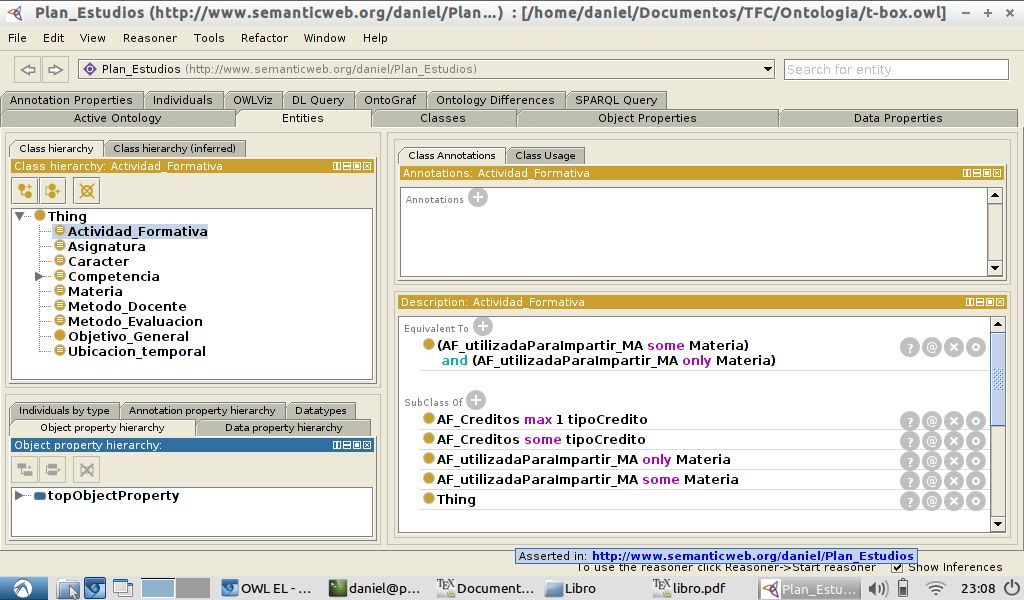
\includegraphics[width=1.00\textwidth]{Imagenes/Herramientas-Protege.png}
	\caption[Prot�g�]{Vista general de Prot�g�.}
\end{figure}


\subsubsection{ACE View}
ACE View\footnote{\url{http://attempto.ifi.uzh.ch/aceview/}} es un editor de reglas y ontolog�as que mediante el uso de Attempto Controlled English\footnote{Attempto Project: \url{http://attempto.ifi.uzh.ch/site/}} permite crear, ver, editar, e interrogar ontolog�as OWL y conjuntos de reglas SWRL. Permite obviar los detalles de OWL y SWRL, ya que el usuario trabaja directamente en ACE, e incluso permite su utilizaci�n simult�nea con otros editores que trabajen sobre OWL.

Permite obtener de manera r�pida una lectura en lenguaje seminatural (ingl�s en este caso). Existe el problema de que el visor no es capaz de interpretar reglas inferidas por el razonador, sino �nicamente aquellas definidas manualmente. De igual modo, no le es posible trabajar con ontolog�as importadas, lo cual limita su uso (para este caso en particular) a una lectura de la traducci�n de la ontolog�a a ACE. Si fuese preciso explotar al m�ximo esta herramienta, podr�amos entonces exportar la ontolog�a a una �nica fuente autocontenida.

A modo de ejemplo, se muestra la parte de la ontolog�a que define \lstinline!Objetivo_General!:

\lstset{language=ace}
\begin{lstlisting}[caption={Descripci�n de la clase Objetivo\_General en ACE},label=ace,captionpos=b]
		Every Objetivo\_General is something.
		Every Objetivo\_General OG\_seCumpleMedianteLaAdquisicionDe\_COes a Competencia.
		Everything that is OG\_seCumpleMedianteLaAdquisicionDe\_COed by an Objetivo\_General is a Competencia.
		Every Competencia CO\_seAdquiereParaCumplir\_OGs an Objetivo\_General.
		Everything that is CO\_seAdquiereParaCumplir\_OGed by something is an Objetivo\_General.
		Every Objetivo\_General is something that OG\_seCumpleMedianteLaAdquisicionDe\_COes nothing but Competencias and that OG\_seCumpleMedianteLaAdquisicionDe\_COes a Competencia.
		Everything that OG\_seCumpleMedianteLaAdquisicionDe\_COes nothing but Competencias and that OG\_seCumpleMedianteLaAdquisicionDe\_COes a Competencia is an Objetivo\_General.
		Everything that is CO\_seAdquiereParaCumplir\_OGed by a Competencia is an Objetivo\_General.
		Everything that OG\_seCumpleMedianteLaAdquisicionDe\_COes something is an Objetivo\_General.
		Every Competencia is something that CO\_seAdquiereParaCumplir\_OGs nothing but Objetivo\_Generals and that CO\_seAdquiereParaCumplir\_OGs an Objetivo\_General.
		Everything that CO\_seAdquiereParaCumplir\_OGs nothing but Objetivo\_Generals and that CO\_seAdquiereParaCumplir\_OGs an Objetivo\_General is a Competencia.
\end{lstlisting}


\section{Razonadores}

Los razonadores son programas software que son capaces de inferir las consecuencias derivadas de un conjunto de hechos o axiomas. Por ejemplo, pueden clasificar un individuo dentro de una clase en funci�n de sus propiedades, inferir relaciones entre dos individuos a trav�s de sus instancias, o detectar insatisfactibilidad en una ontolog�a. Existen multitud de razonadores, cada uno con unas caracter�sticas determinadas. Los distintos razonadores var�an en funci�n de la expresividad que soportan, del algoritmo que utilizan, si soportan reglas (con formatos propios o est�ndares como SWRL\footnote{\url{http://www.w3.org/Submission/SWRL/}}), o del tipo de licencia otorgada para su distribuci�n.

\subsubsection{FaCT++}
Es una mejora sobre el anterior razonador FaCT, que hace uso de los mismos algoritmos que �ste, pero con una implementaci�n mejorada. Adem�s, FACT++\footnote{\url{http://owl.man.ac.uk/factplusplus/}} est� creado utilizando el lenguaje C++ lo que ha incrementado su eficacia y su portabilidad. Ha sido desarrollado por la Universidad de Manchester y se instala de forma predeterminada junto con Prot�g�.

FaCT++ no soporta el uso de ``built-in primitive datatypes''\footnote{\url{http://www.w3.org/TR/2004/REC-xmlschema-2-20041028/\#built-in-primitive-datatypes}} y existe, en la p�gina del razonador \footnote{\url{http://code.google.com/p/factplusplus/issues/detail?id=9}} una cuesti�n abierta por este asunto, pendiente de encontrar soluci�n.


\subsubsection{HermiT}
Se trata de un razonador de c�digo abierto bajo licencia LGPL para ontolog�as OWL. HermiT\footnote{\url{http://www.hermit-reasoner.com/}} es capaz de determinar si una ontolog�a es o no consistente, identifica relaciones del tipo ``es un'', clasifica elementos de la ontolog�a, entre otras capacidades. Hace uso de un nuevo algoritmo que lo hace m�s eficaz que cualquier otro utilizado anteriormente, y cumple con los est�ndares OWL2\cite{w3c.org-owl2primer}. La versi�n utilizada en el desarrollo de la ontolog�a es la 1.3.8.

\begin{figure}[h!]
	\centering
		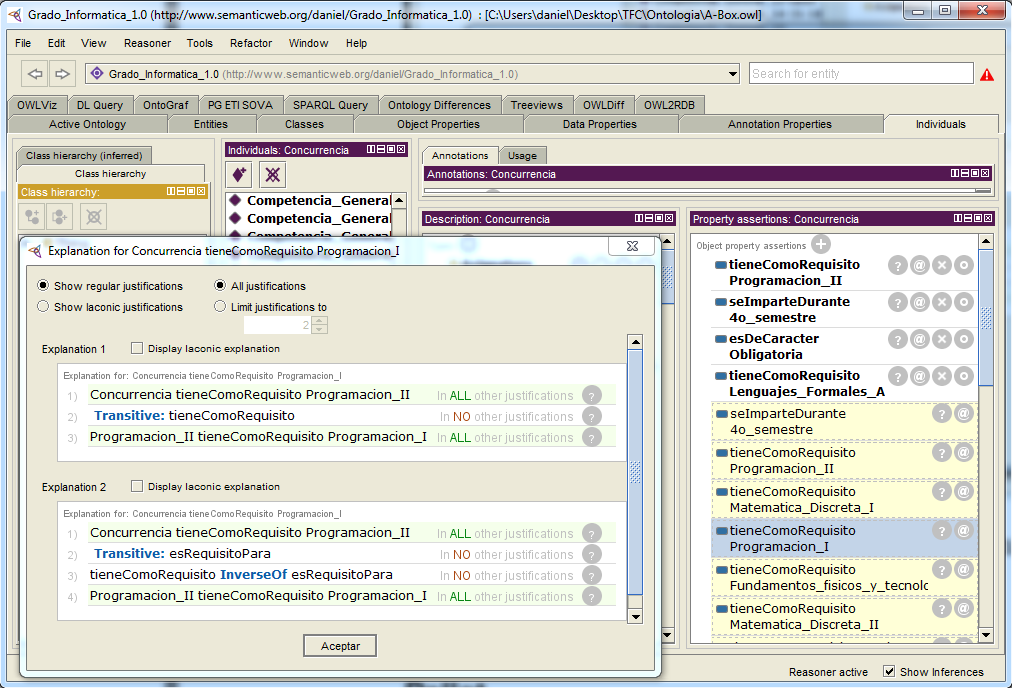
\includegraphics[width=1.00\textwidth]{Imagenes/Herramientas-HermiT.png}
	\caption[HermiT]{Ejemplo de razonamiento usando HermiT}
\end{figure}

\subsubsection{RacerPro}
RacerPro\footnote{\url{http://www.racer-systems.com/products/racerpro/}} es el nombre comercial del razonador para OWL llamado RACER (Renamed ABox and Concept Expression Reasoner). El razonador puede usarse para razonamiento sobre l�gica descriptiva, desarrollo de ontolog�as y web sem�ntica basada en OWL, repositorio de informaci�n para la web sem�ntica, e incluso para el trabajo con l�gica modal.  Existe un plugin para Prot�g� llamado RacerProTG\footnote{\url{http://protegewiki.stanford.edu/wiki/RacerProTG}} que trabaja de forma autom�tica con la �ltima versi�n disponible del razonador RacerPro (existe una licencia gratuita y permanente para el uso del plugin junto con Prot�g�). 

\subsubsection{Pellet}
Pellet\footnote{\url{http://clarkparsia.com/pellet}} es un razonador para ontolog�as OWL DL, con soporte para OWL2 e incluso OWL2 EL\cite{w3c.org-owl2profiles}, que a�ade la particularidad de permitir razonamiento incremental (lo que permite, ante cambios realizados en la ontolog�a --- bien en la jerarqu�a de clases, bien en los individuos --- no tener que realizar todo el proceso de razonamiento desde cero). Pellet se ofrece con dos licencias distintas, en funci�n de la finalidad a la que se destine. 
Pellet permite el razonamiento con ontolog�as OWL-Full, e incluso cambiar de manera sencilla el comportamiento del razonador para que trabaje sobre hip�tesis de mundo cerrado, o con suposici�n de nombres �nicos. Tambi�n es posible el razonamiento con reglas SWRL (que no se aplicar�n a individuos an�nimos de la ontolog�a).
Sin embargo, su comportamiento resulta mucho m�s pesado que los otros razonadores, y mientras que HermiT es capaz de clasificar la ontolog�a y encontrar inconsistencias en apenas 28 segundos, tras muchos minutos m�s Pellet a�n no ha logrado concluir la clasificaci�n. 


\section{Visores}
Los visores nos permiten visualizar la informaci�n de manera m�s sencilla, de modo que aumenta la comprensi�n de la informaci�n y la claridad de la misma. Gracias a ellos podemos obtener diferentes puntos de vista de la ontolog�a, y crear un ambiente m�s amigable para el trabajo con las ontolog�as.

\subsubsection{OWLDoc}
OWLDoc\footnote{\url{http://code.google.com/p/co-ode-owl-plugins/wiki/OWLDoc}} es un plugin de Prot�g� que permite exportar la informaci�n contenida en la ontolog�a a HTML, de modo que la visualizaci�n de la informaci�n es m�s amena y flexible. OWLDoc exporta toda la informaci�n que contiene la ontolog�a. En la documentaci�n que genera y por la que podemos navegar encontramos todo lo relativo a clases, propiedades sobre objetos, propiedades sobre datos, y adem�s, sobre los individuos de la ontolog�a e incluso sobre los tipos de datos que hemos utilizado en la misma. En definitiva, se trata de un salto cualitativo en el modo de explorar la ontolog�a, con respecto a las herramientas vistas hasta ahora.

\begin{figure}[!h]
	\centering
		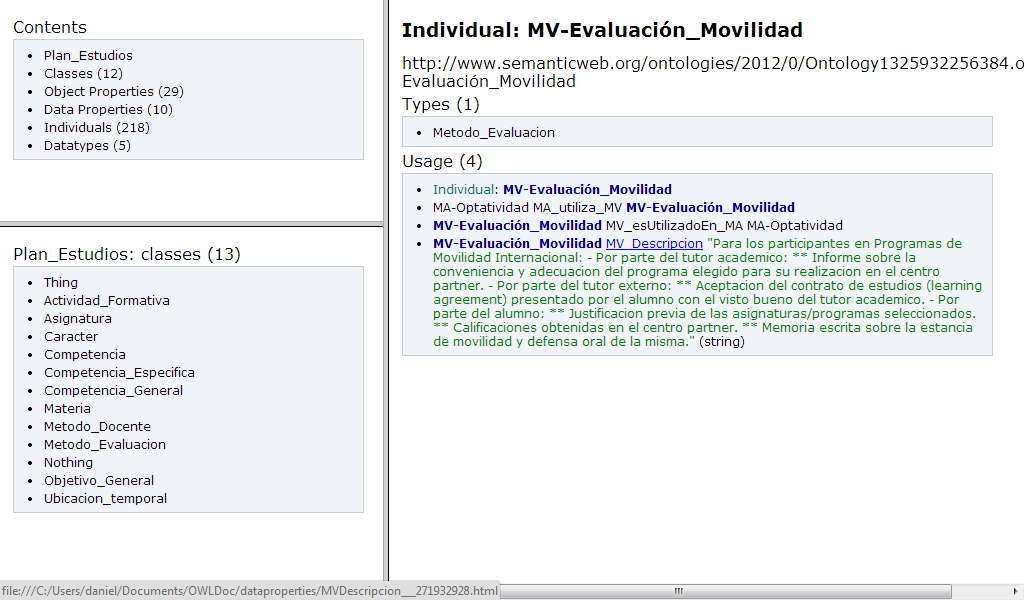
\includegraphics[width=1.00\textwidth]{Imagenes/Herramientas-OWLDoc.png}
	\caption[OWLDoc]{Vista del individuo \lstinline!MV-Evaluacion_Movilidad!}
\end{figure}

\subsubsection{CloudViews}
Este plugin\footnote{\url{http://code.google.com/p/co-ode-owl-plugins/wiki/CloudViews}} nos permite ver la ontolog�a como una nube de tags. Podemos ver las diferentes clases, propiedades e individuos y representarlos en una nube de tags. Los tags se pueden ordenar en funci�n del uso, de su profundidad, relaciones, restricciones y otras caracter�sticas, de modo que es muy f�cil e intuitivo hacerse r�pidamente una idea de los elementos m�s importantes de una ontolog�a.

Adem�s, permite exportar los resultados a formato html que luego pueden visualizarse en un navegador web. Los tags entonces se convierten en hiperv�nculos, que usados en conjunci�n con otras herramientas como OWLDOC nos permitir�a llegar desde la ontolog�a hasta las definiciones de cada uno de sus componentes a trav�s de enlaces html.

\begin{figure}[!h]
	\centering
		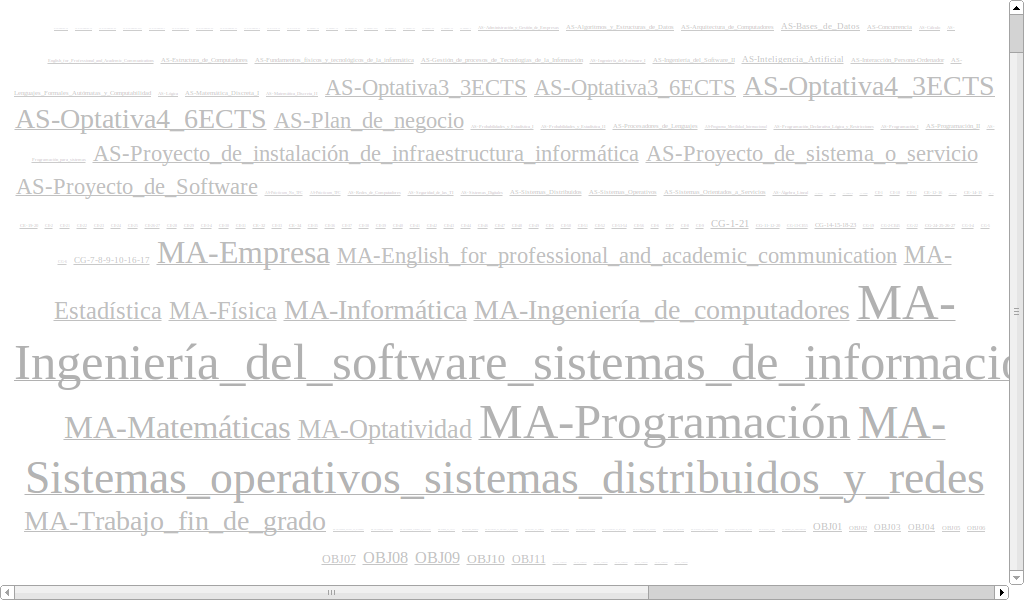
\includegraphics[width=1.00\textwidth]{Imagenes/Herramientas-cloudview.png}
	\caption[CloudViews]{Vista en un navegador a pantalla completa de la nube de tags}
\end{figure}

\subsubsection{Matrix}
El plugin Matrix\footnote{\url{http://code.google.com/p/co-ode-owl-plugins/wiki/MatrixViews}} nos permite tener una visi�n de la ontolog�a en forma de tabla, seleccionando aquella informaci�n que de las diferentes clases, propiedades e individuos nos interesa. Incluso es posible, desde la propia tabla, incluir informaci�n en la ontolog�a, lo que la convierte en muy �til para completar informaci�n. Tiene el inconveniente de que no es capaz de trabajar con axiomas inferidos, por lo que pierde una gran parte de su utilidad, ya que toda la informaci�n debe estar insertada en la ontolog�a.

\begin{figure}[!h]
	\centering
		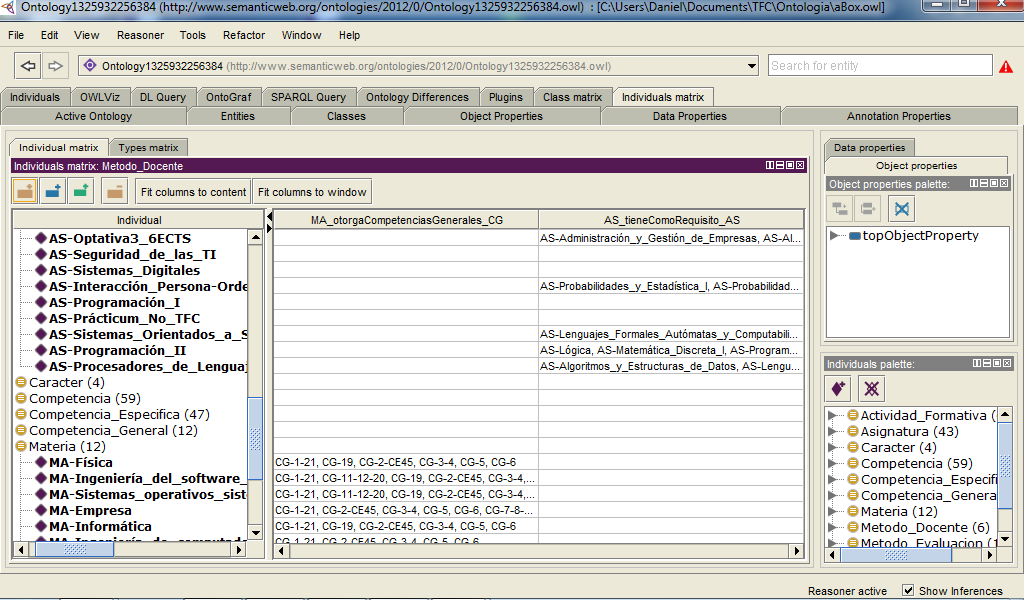
\includegraphics[width=1.00\textwidth]{Imagenes/Herramientas-matrix.png}
	\caption[Matrix: Individuos]{Vista de los individuos}
\end{figure}
\begin{figure}[!h]
		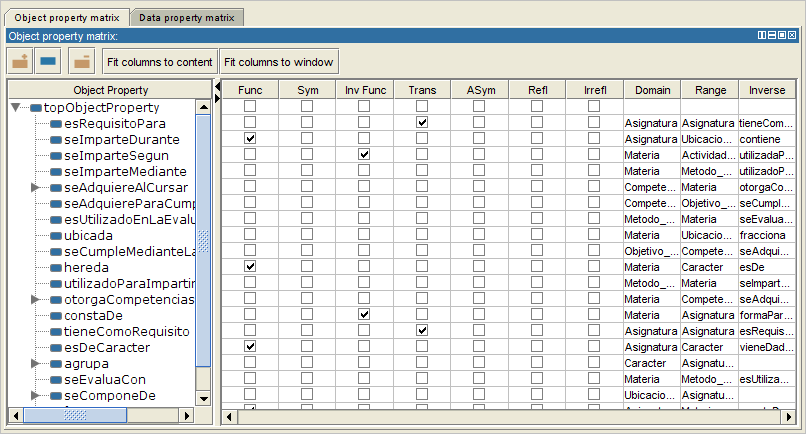
\includegraphics[width=1.00\textwidth]{Imagenes/Herramientas-matrix2.png}
	\caption[Matrix: Propiedades]{Vista de las propiedades}
\end{figure}

\subsubsection{NavigOWL}
NavigOWL\footnote{\url{http://klatif.seecs.nust.edu.pk/navigowl/index.html}} es una herramienta de visualizaci�n especialmente dise�ada para explorar ontolog�as y permitir una mejor comprensi�n de su estructura. Los gr�ficos pueden mostrarse en pantalla seg�n diferentes t�cnicas de modo que sea m�s f�cil comprender la importancia de cada nodo, al aparecer este de mayor tama�o. Tambi�n es posible mostrar u ocultar las etiquetas de los diferentes nodos o redistribuirlos en el lienzo. La herramienta incorpora una funci�n de b�squeda que permite localizar en el grafo cualquier nodo de la ontolog�a, lo que tambi�n facilita el examen de la misma. 

La herramienta est� disponible como archivo java ejecutable y tambi�n como un plugin para Prot�g�.

\begin{figure}[!h]
	\centering
			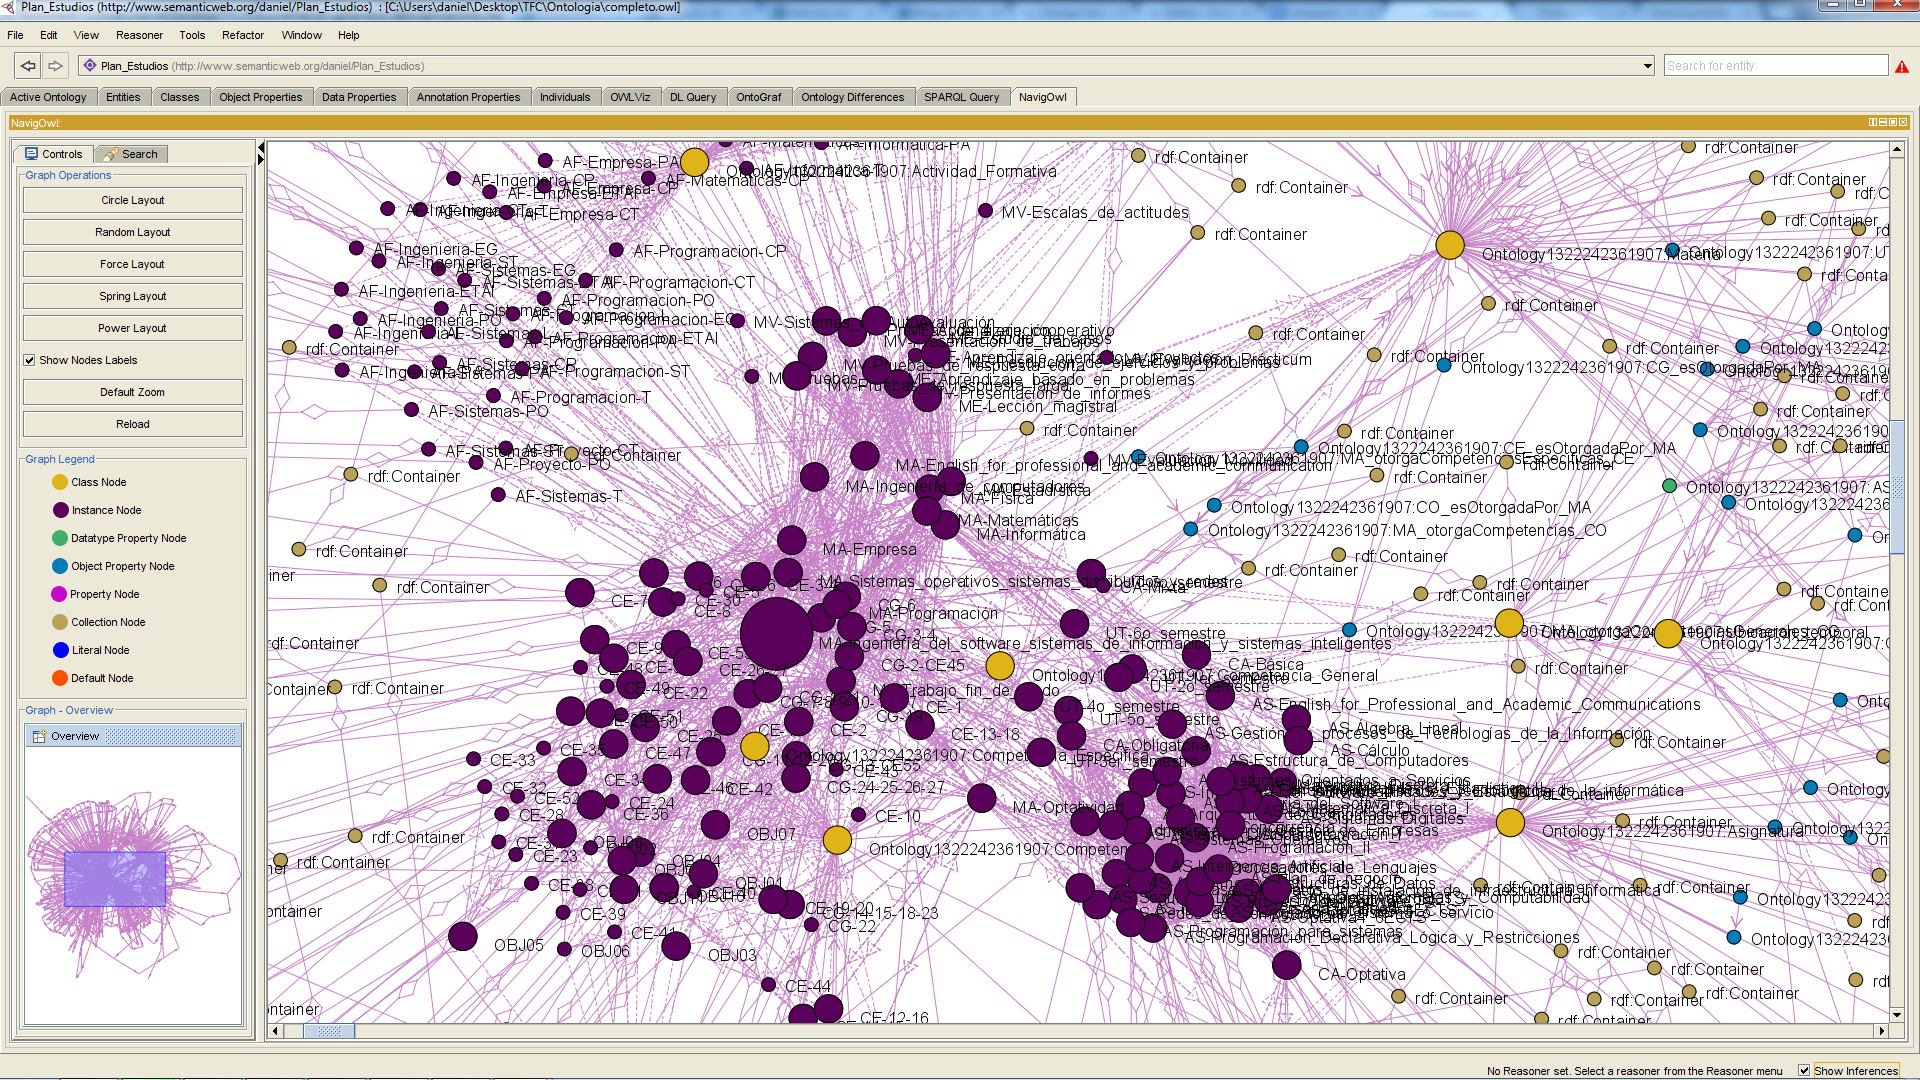
\includegraphics[width=1.00\textwidth]{Imagenes/Herramientas-NavigOwl.png}
		\caption[NavigOWL]{Vista de parte de la ontolog�a a trav�s del visor NavigOWL}
\end{figure}

\subsubsection{Ontograf}
Ontograf\footnote{\url{http://protegewiki.stanford.edu/wiki/OntoGraf}} es otro visor de ontolog�as. A diferencia de NavigOWL, todos los nodos tienen la misma representaci�n, sin poder establecer a priori una clasificaci�n en funci�n de su importancia, pero a cambio resulta mucho m�s �gil de manejar que NavigOWL, ya que en ontolog�as grandes como la nuestra, no resulta una aplicaci�n tan pesada de mover. Se puede elegir si deseamos que nos muestre individuos o clases, cuales nos debe mostrar e incluso podemos ocultar clases o individuos que est�n relacionados mediante una propiedad en particular.

Admite las relaciones de subclases, individuos, dominio, rango, pertenencia, etc de las propiedades y equivalencias. Tambi�n se pueden personalizar, para cada tipo de nodo, la informaci�n que queremos visualizar.

\begin{figure}[!h]
	\centering
		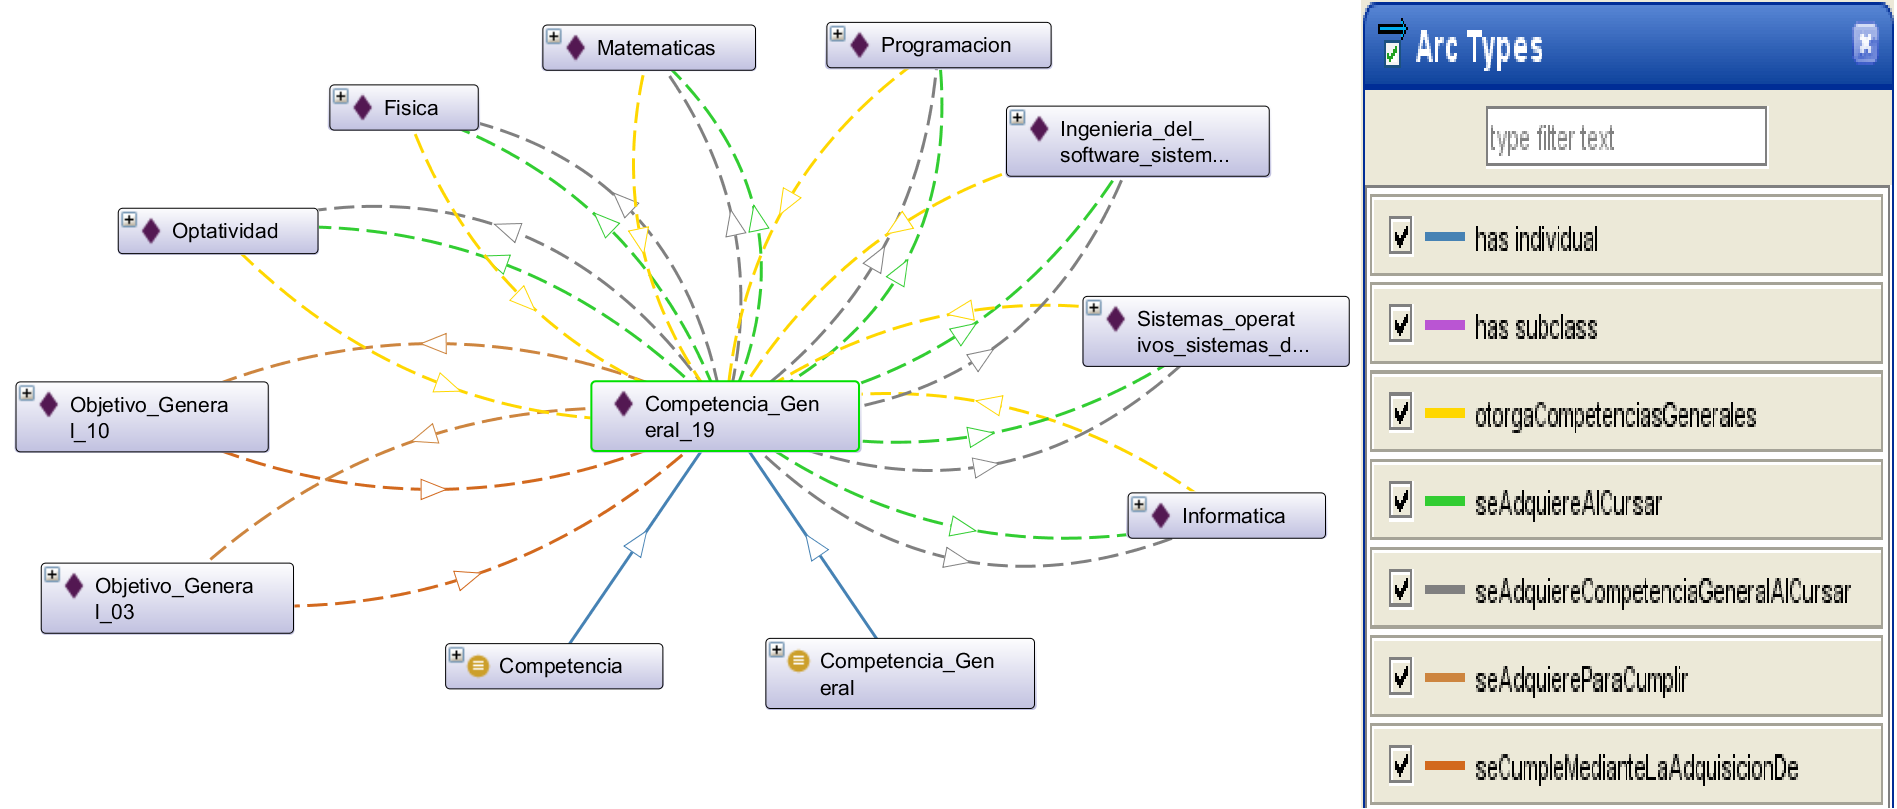
\includegraphics[width=1.00\textwidth]{Imagenes/Herramientas-OntoGraf.png}
		\caption[OntoGraf]{Vista de una competencia en OntoGraf.}
\end{figure}

\subsubsection{OWLGrEd}
OWLGrEd\footnote{\url{http://owlgred.lumii.lv/}} es un editor gr�fico para ontolog�as OWL. Permite visualizar ontolog�as existentes en diagramas UML y la creaci�n y desarrollo de ontolog�as desde el propio entorno gr�fico, sin necesidad de otros editores o software adicional. Las ontolog�as creadas pueden ser exportadas a Prot�g� para comprobar su consistencia, realizar una clasificaci�n, etc, o tambi�n importadas desde Prot�g� a la herramienta. Podemos personalizar que entidades mostrar en el diagrama, cambiar la disposici�n de los distintos elementos en el mismo, o el estilo gr�fico. Adem�s, podemos generar archivos gr�ficos y documentaci�n en html para poder utilizar como apoyo para otros trabajos.

Es un modo de ver la estructura de la ontolog�a muy r�pidamente, pero cuenta con el inconveniente de que, en ontolog�as grandes con muchos individuos, el tiempo de carga la hacen inviable. Adem�s, el software lanza excepciones no controladas en tiempo de ejecuci�n al cargar la ontolog�a con todos los individuos, pero solamente muestra un error gen�rico, con lo cual resulta del todo inviable averiguar el motivo del fallo.

\begin{figure}[!h]
	\centering
		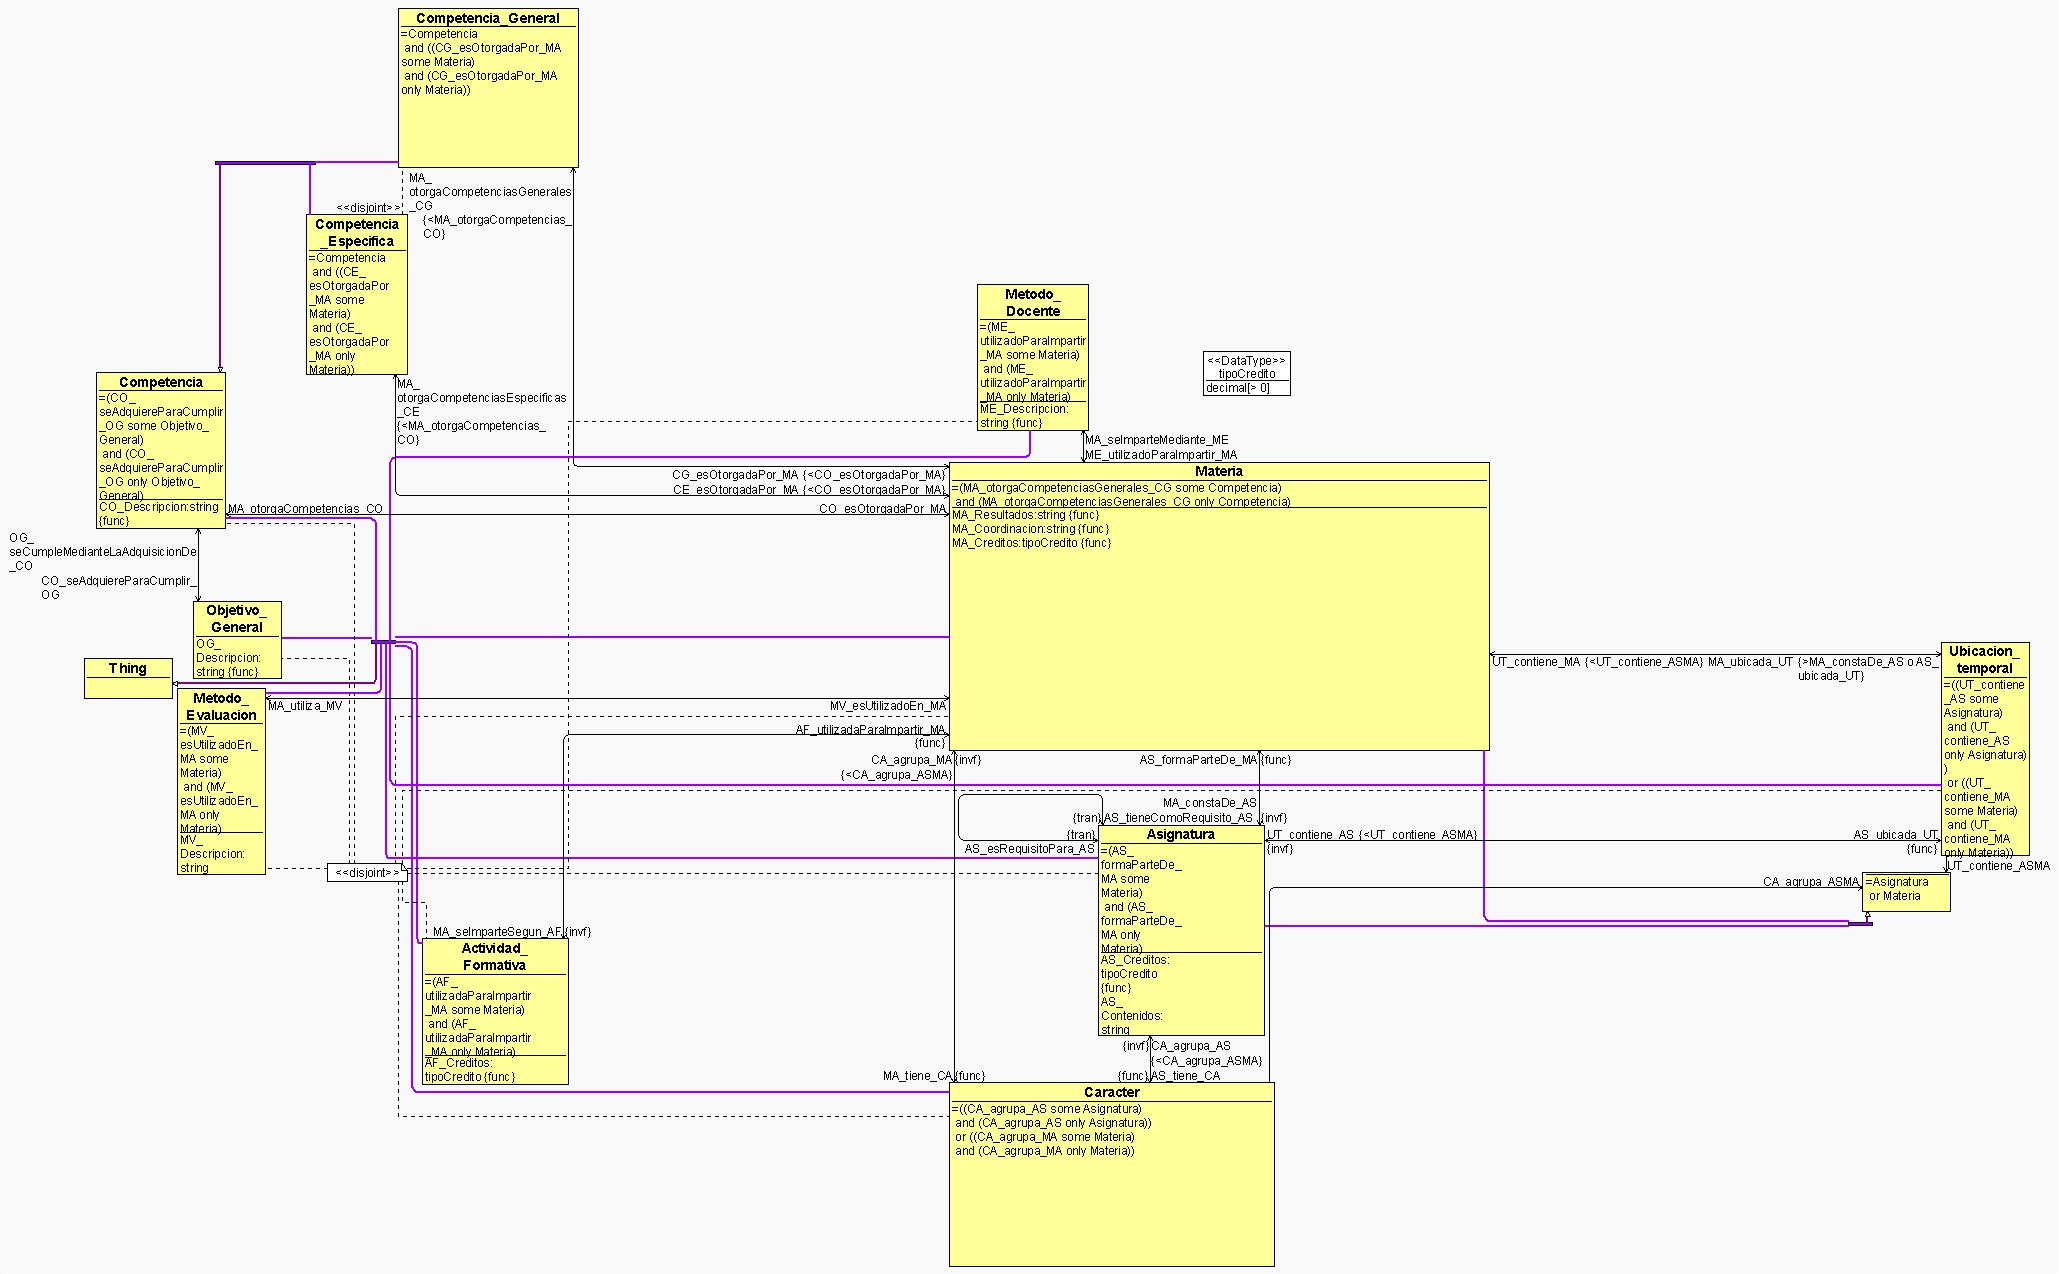
\includegraphics[width=1.00\textwidth]{Imagenes/Herramientas-OWLGrEd.png}
	\caption[OWLGrEd]{Diagrama UML parcial de la TBox}
\end{figure}

\subsubsection{SOVA}
SOVA\footnote{\url{http://protegewiki.stanford.edu/wiki/SOVA}} es un plugin de Prot�g� desarrollado por la universidad de Gdansk que permite la visualizaci�n de ontolog�as al completo. Gracias a SOVA, podemos tener en un mismo esquema clases, individuos y relaciones. 

SOVA tiene dos modos de trabajo. En el primer modo obtener una visualizaci�n interactiva de la ontolog�a en disposici�n radial, con todas sus clases, individuos, propiedades, etc, pero sin ninguna clasificaci�n. Es decir, la visualizaci�n se limita a la lectura del fichero OWL, pero no se realiza sobre �l ninguna labor de clasificaci�n o razonamiento previo. En el segundo modo, la herramienta realiza una clasificaci�n previa utilizando el razonador HermiT y muestra a continuaci�n una jerarqu�a de clases y los individuos que las componen, pero sin mostrar las propiedades mediante las cuales los individuos de las diferentes clases se relacionan.

\begin{figure}[!h]
	\centering
		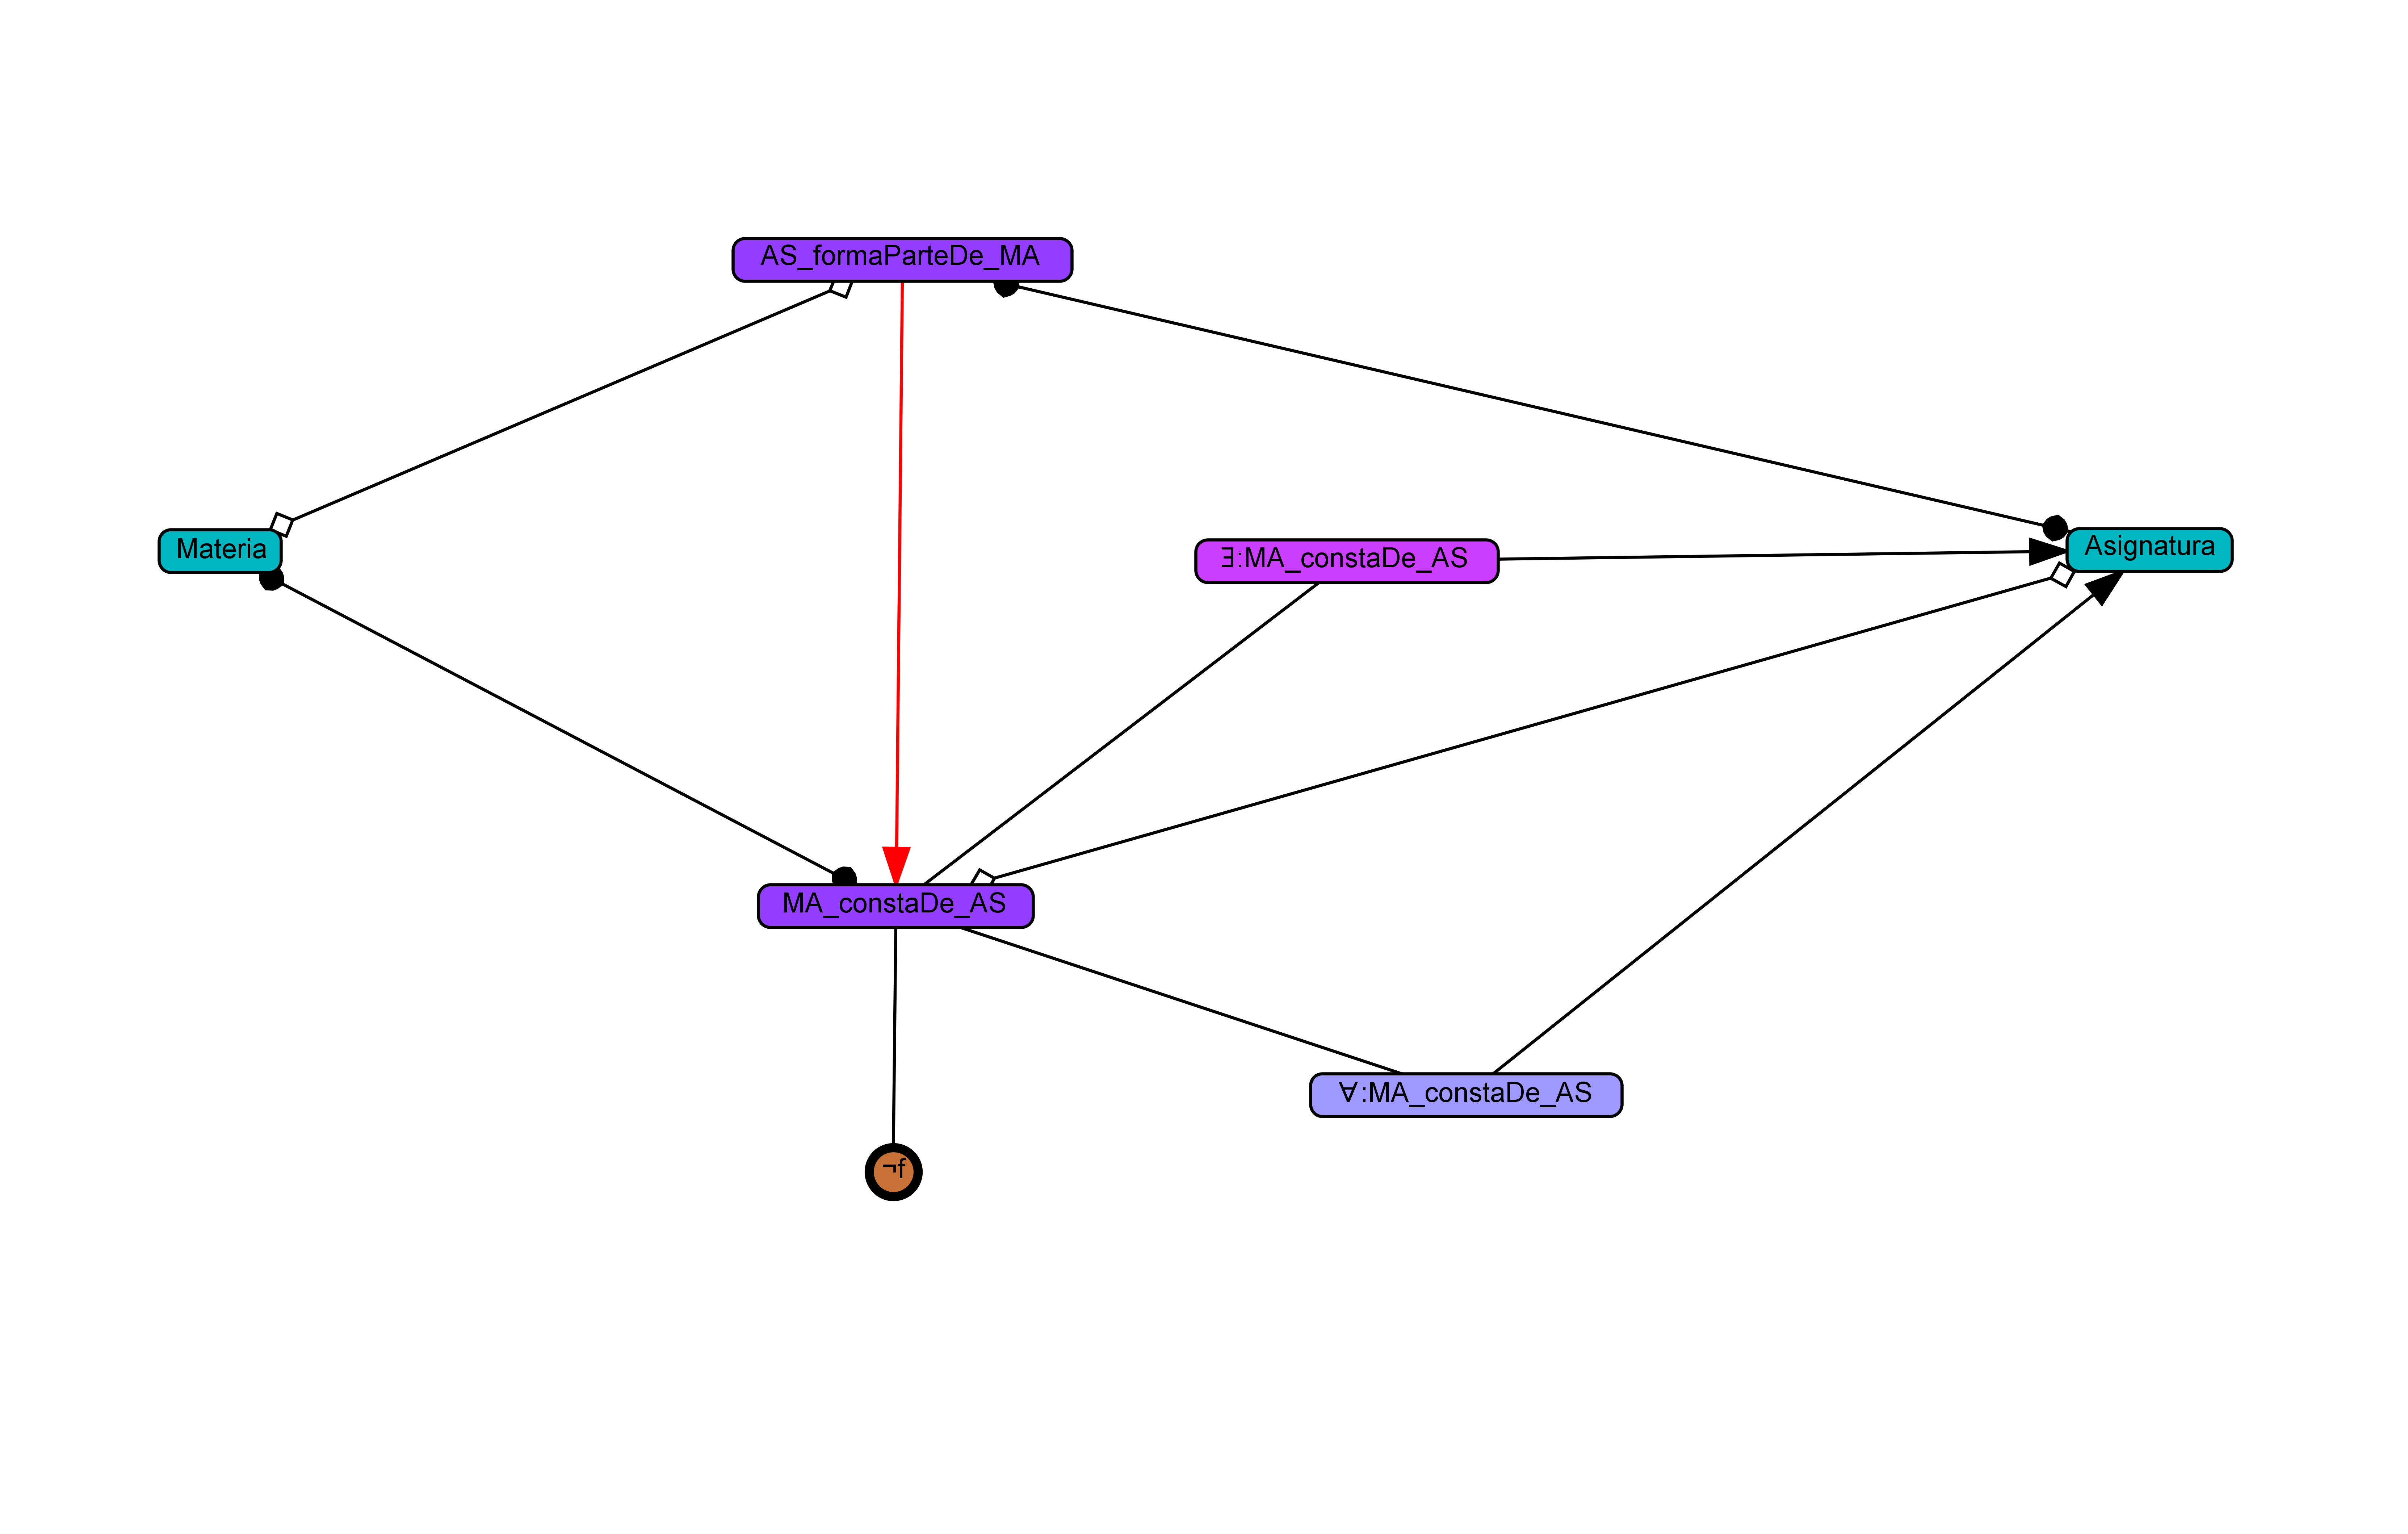
\includegraphics[width=1.00\textwidth]{Imagenes/Herramientas-SOVAvis.png}
	\caption[SOVA - Interactiva]{Visualizaci�n de las relaciones entre Materia y Asignatura}
\end{figure}
\begin{figure}[!h]
	\centering
		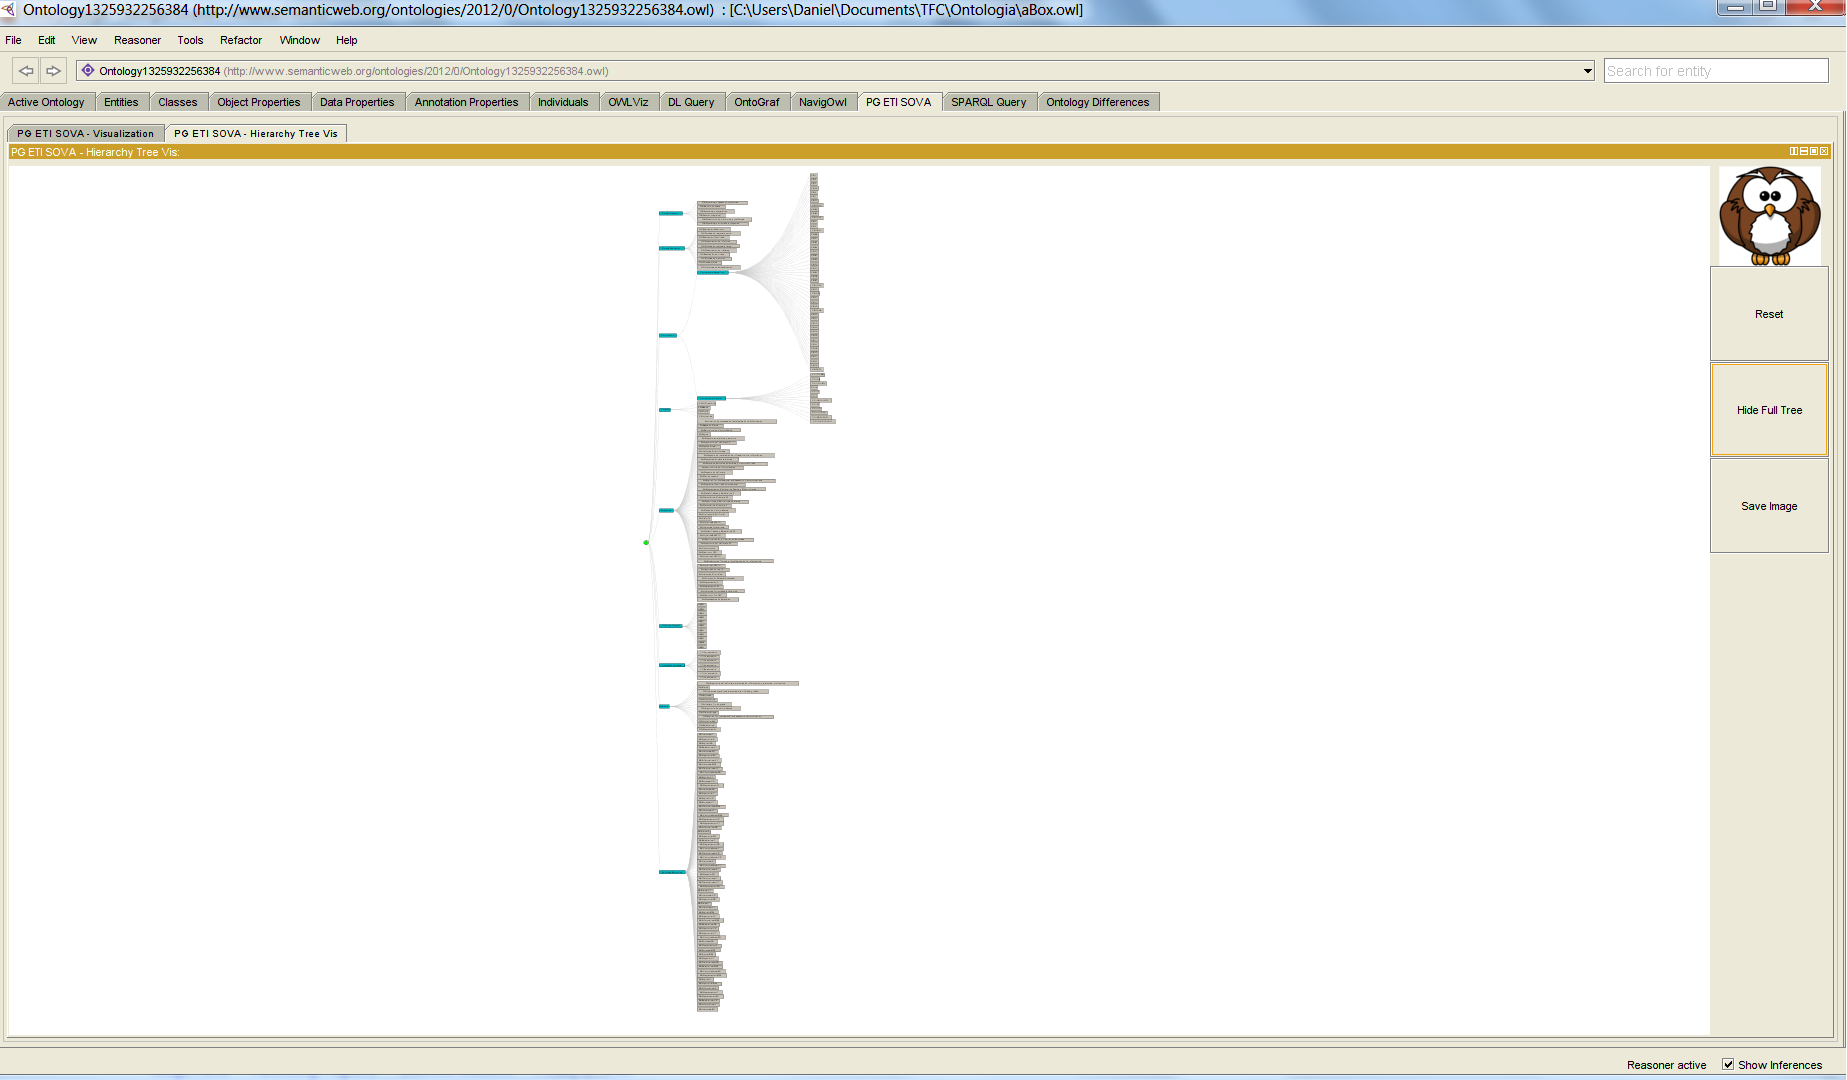
\includegraphics[width=1.00\textwidth]{Imagenes/Herramientas-SOVAhie.png}
	\caption[SOVA - Jerarqu�a]{Visualizaci�n jerarquizada de las clases e individuosde la ontolog�a}
\end{figure}

\subsubsection{DL-Query}
Se trata de un plugin de Prot�g� que nos permite, mediante el uso de un razonador, realizar comprobaciones acerca de la consistencia de la ontolog�a y de las asunciones que el razonador realiza. DL-Query\footnote{\url{http://protegewiki.stanford.edu/wiki/DL\_Query}} tambi�n es �til para probar la pertenencia a una y otra clase de cualquier descripci�n arbitraria, sin necesidad de tener que crear una clase definida para ello, y si esa consulta se realiza muy a menudo, es posible almacenar dicha consulta dentro de la propia ontolog�a en forma de clase definida o an�nima, con lo que resulta mucho m�s �gil el poder realizar la misma comprobaci�n sobre la ontolog�a de manera repetida. En general, es capaz de contestar preguntas realizadas acerca de la ontolog�a utilizando el motor de inferencia. DL-Query utiliza sintaxis Manchester para la interacci�n con la ontolog�a.

\begin{figure}[!h]
	\centering
		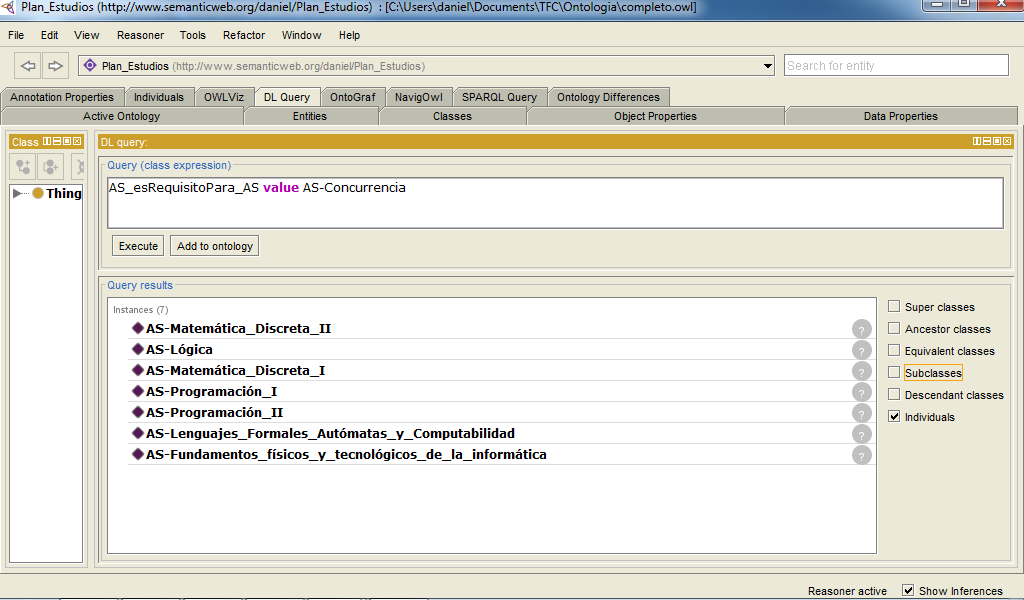
\includegraphics[width=1.00\textwidth]{Imagenes/Herramientas-DLQuery.png}
	\caption[DL-Query]{``�Qu� valores son requisitos para poder cursar Programaci�n Concurrente?''}
\end{figure}

\subsubsection{Cardinality View}
Es un plugin, integrado en Prot�g� que nos permite visualizar las restricciones de cardinalidad de un modo mas amigable, sobre todo para personas no familiarizadas con la sintaxis de Prot�g�. Cardinality View\footnote{\url{http://code.google.com/p/co-ode-owl-plugins/wiki/Cardinality}} nos permite no s�lo visualizar esas restricciones, sino que incluso podemos editar dichas restricciones, a�adir unas nuevas, o eliminar las ya existentes. Admite restricciones sobre clases, propiedades de datos, constantes de propiedades de datos e incluso de individuos.

\begin{figure}
	\centering
		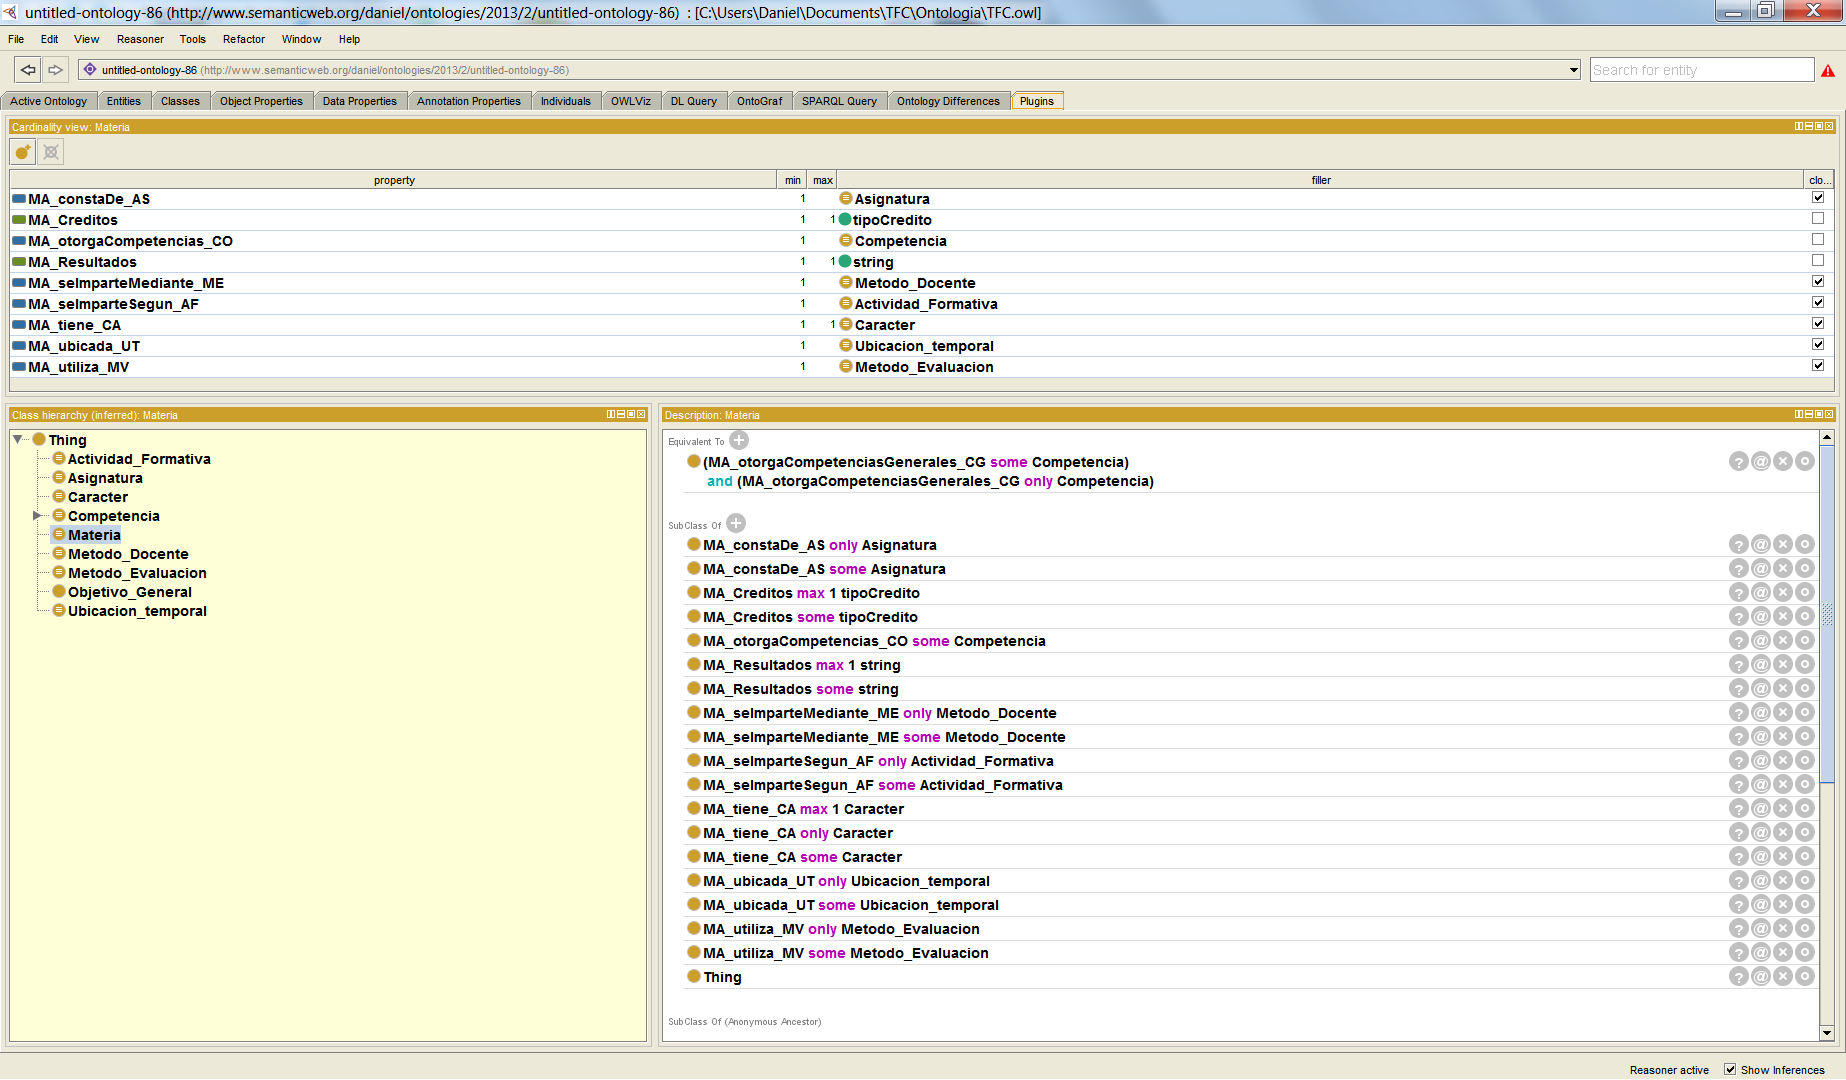
\includegraphics[width=1.00\textwidth]{Imagenes/Herramientas-CardinalityView.png}
	\caption[Cardinality View]{Vista de la clase \lstinline!Materia!}
\end{figure}

\subsubsection{Outline and Existential Tree Views}
Este\footnote{\url{http://code.google.com/p/co-ode-owl-plugins/wiki/OutlineView}} plugin nos permite visualizar las relaciones existenciales de la ontolog�a en forma de �rbol, a partir de cualquier nodo, y pudiendo colgar en �l las propiedades de objetos y datos. De este modo, podemos obtener una visi�n de la ontolog�a desde la parte de la misma que en cada momento nos resulte de inter�s, facilitando la comprensi�n y el acceso a la informaci�n.

\begin{figure}[!h]
	\centering
				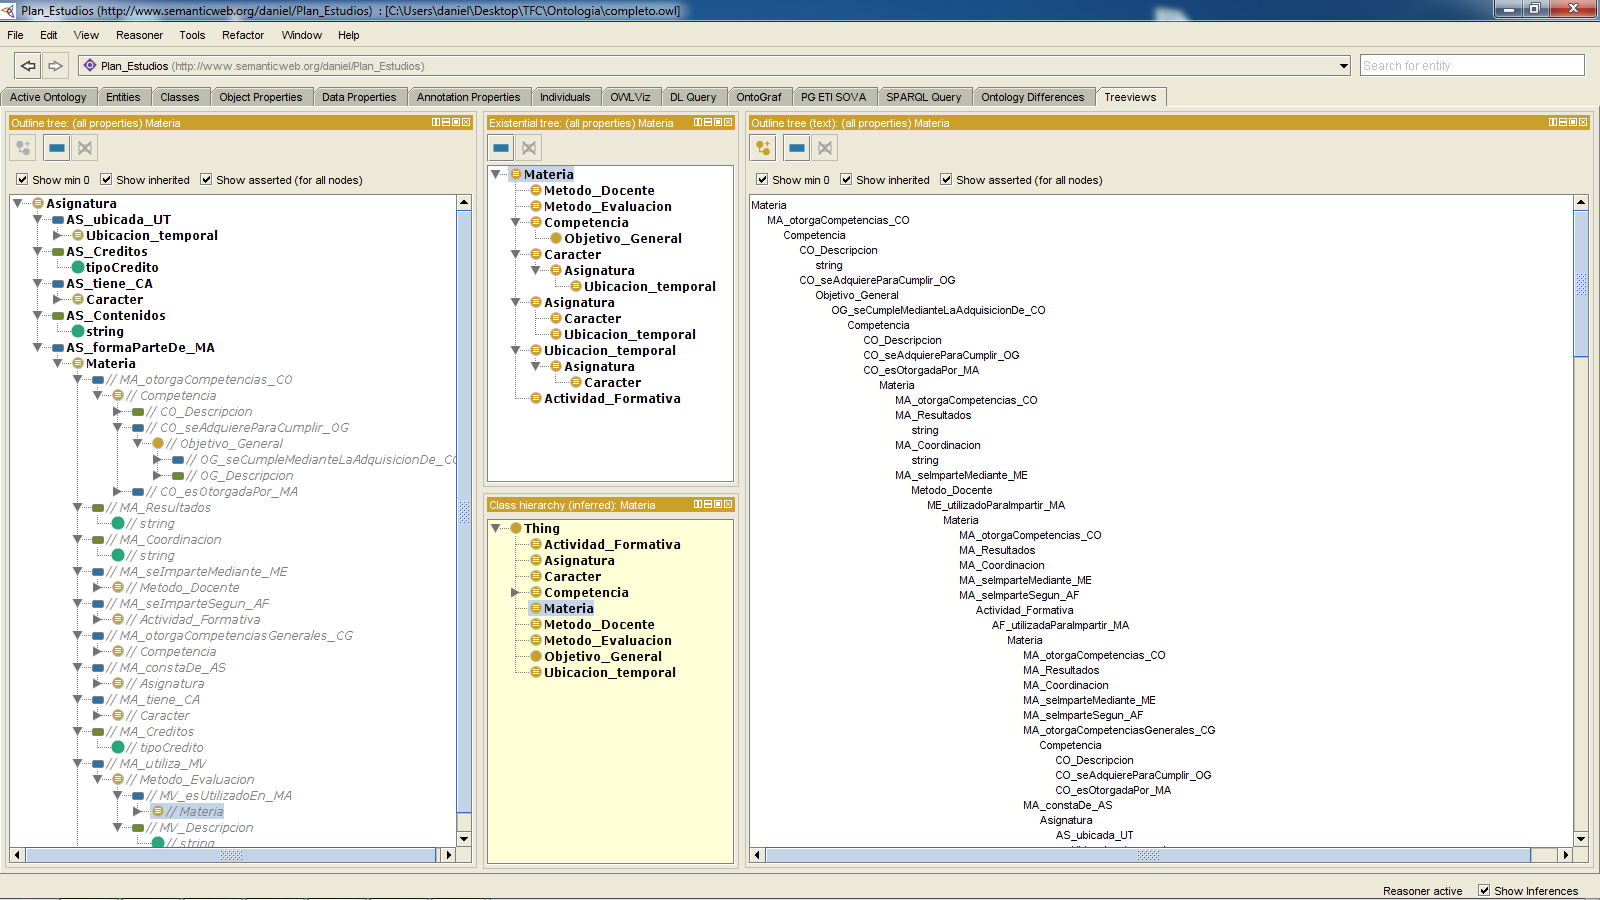
\includegraphics[width=1.00\textwidth]{Imagenes/Herramientas-ExistentialTree.png}
	\caption[Outline and existential Tree Views]{�rbol generado a partir de \lstinline!Asignatura!}
\end{figure}


\subsubsection{OWLViz}
Plugin\footnote{\url{http://protegewiki.stanford.edu/wiki/OWLViz}} de Prot�g�, muy b�sico, que permite navegar �nicamente sobre las clases de la ontolog�a. No permite acceder a informaci�n contenida en las clases, o a las relaciones entre ellas, limit�ndose a mostrar relaciones del tipo ``es un''. 

\subsubsection{OWLPropViz}
Plugin basado en OWLViz, que adem�s de mostrar relaciones del tipo ``es-un'', nos ense�a relaciones de equivalencia, clases disjuntas, y otras propiedades sobre objetos definidas en la ontolog�a. 
Por desgracia, no he sido capaz de lograr que funcione. OWLPropViz\footnote{\url{http://protegewiki.stanford.edu/wiki/OWLPropViz}} figura como compatible �nicamente con la versi�n 4.0 de Prot�g�, y no se ha logrado que funcione en versiones superiores como 4.1 o 4.2. 

\subsubsection{OWLDiff}
Herramienta disponible para uso dentro de Prot�g� en forma de plugin o como un programa individual que nos permite comparar dos ontolog�as, mostr�ndonos las diferencias y similitudes entre ellas, unirlas en una �nica ontolog�a, y realizar inferencias sobre ellas utilizando el razonador Pellet. Con OWLDiff\footnote{\url{http://semanticweb.org/wiki/OWLDiff}} podemos ver el resultado de la comparativa en forma de axiomas o inserciones de la ontolog�a y cada uno de ellos en sintaxis DL o Manchester. Tambi�n es posible desde la misma aplicaci�n exportar axiomas desde una ontolog�a hacia la otra.
Adem�s tiene la posibilidad de integrarse en varios sistemas de control de versiones, como Subversion, lo que facilita el trabajo sobre la ontolog�a por un amplio grupo de gente. 

\begin{figure}[!h]
	\centering
		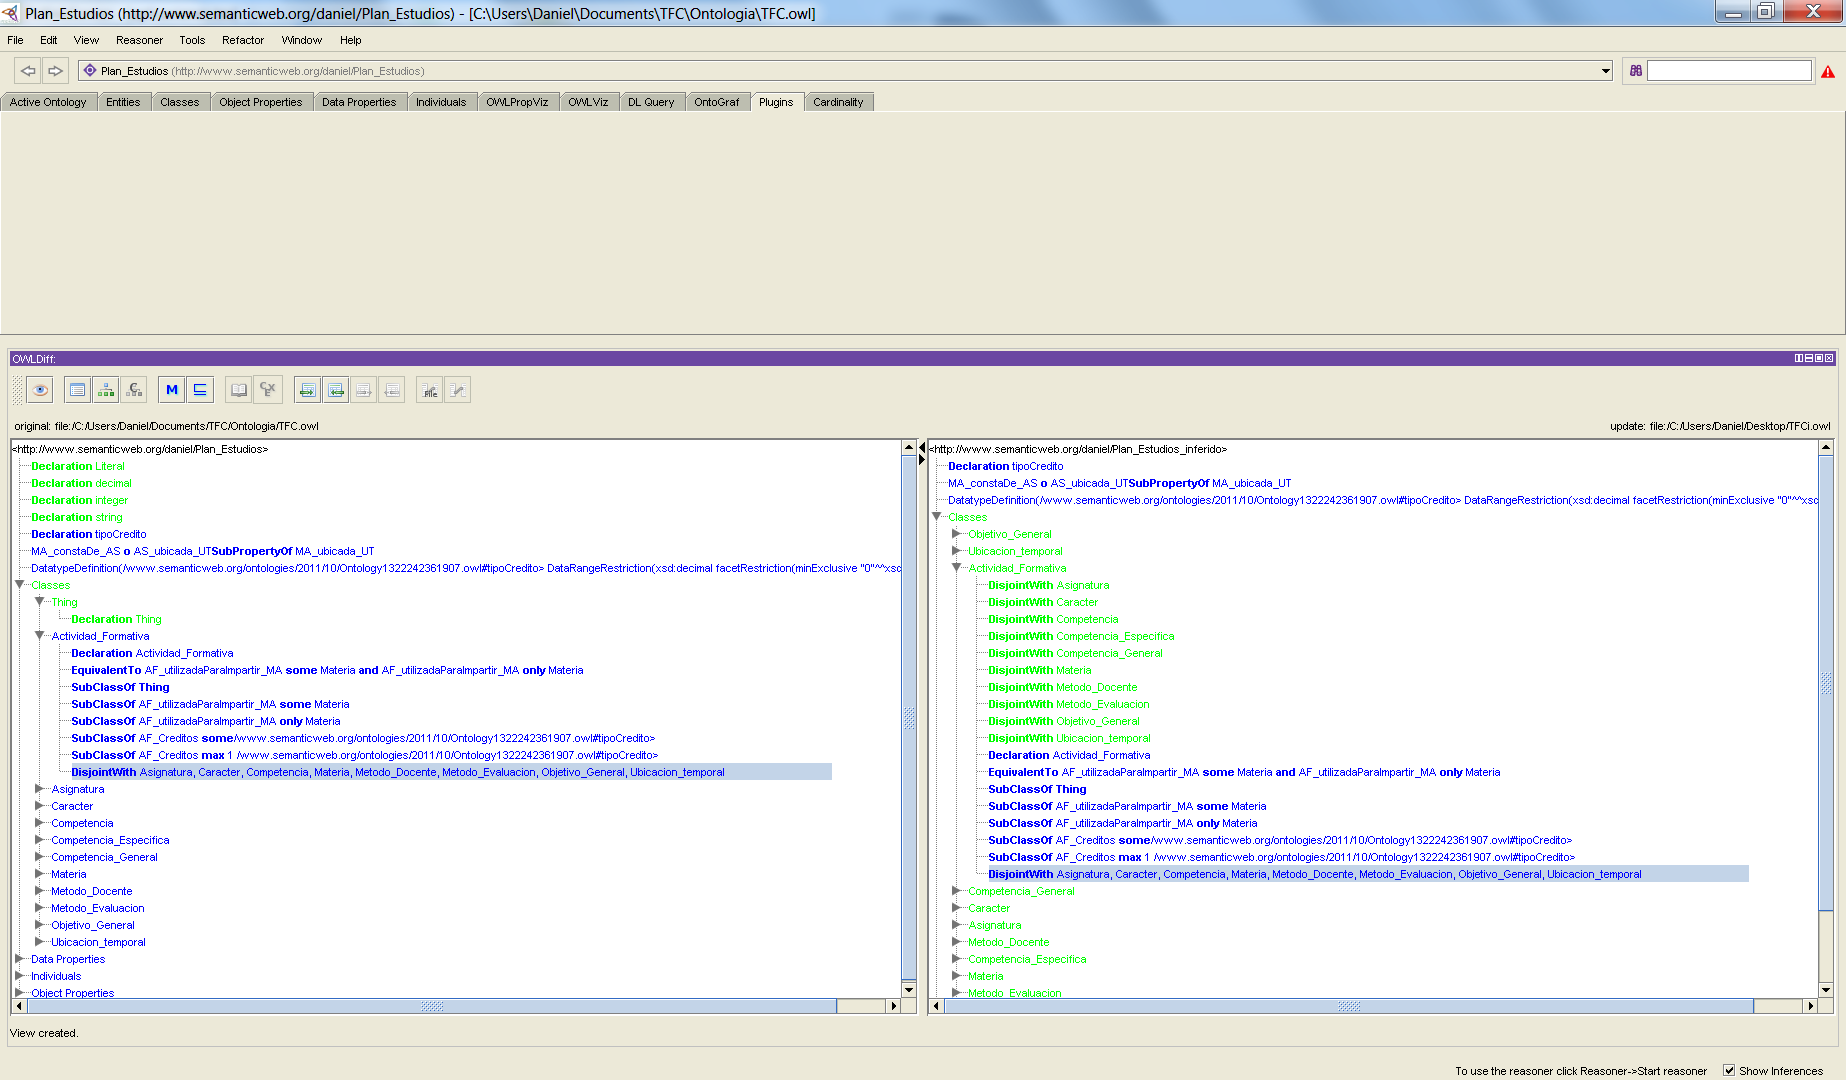
\includegraphics[width=1.00\textwidth]{Imagenes/Herramientas-OWLdiff.png}
	\caption[OWLDiff]{Muestra de dos ontolog�as distintintas analizadas por la herramienta}
\end{figure}


\section{Transformaci�n de datos}

\subsubsection{OWL2ToRDB} Es un plugin para Prot�g� que permite transformar ontolog�as OWL2 en bases de datos relacionales. Por desgracia, el plugin no funciona correctamente ni con las versiones de java disponibles junto con Prot�g�, ni con otras versiones actuales de java y no se distribuye ning�n tipo de documentaci�n ni existe p�gina web del autor u otras donde se mencione la aplicaci�n, a donde podamos dirigirnos para obtener m�s informaci�n acerca del error. Nos parec�a muy interesante el poder exportar la ontolog�a a una base de datos y trabajar con herramientas especializadas sobre ella. 

\subsubsection{Protege-OWL Code Generator} Creado por los desarrolladores de Prot�g�, este plugin busca facilitar el desarrollo de aplicaciones a partir de ontolog�as. El plugin genera, a partir de una ontolog�a, c�digo en java, con el cual podemos trabajar directamente. A modo de ejemplo, se muestra parte del c�digo generado por la versi�n 1.0.0 para la clase \lstinline!Materia!

\lstinputlisting[caption={C�digo generado para la clase \lstinline!Materia!},captionpos=b,label=owl-code,language=Java,mathescape=false,firstline=1, lastline=50]{codigo/Materia.java}

\section{Control de versiones}

\subsubsection{Prot�g�HGDB}
Es un software que permite la colaboraci�n de un equipo y realizar el control de versiones desde dentro de Prot�g�. Este plugin\footnote{\url{http://sharegov.org/\#!../protegehgdb/owltools.html}} ha sido desarrollado por el condado de Miami-Dade, para el control de versiones y salvaguarda de la ontolog�a en desarrollo. Haciendo uso de hipergrafos dirigidos, es capaz de realizar el control de versiones a nivel de la ontolog�a, por lo que las operaciones de salvaguarda y restauraci�n trabajan directamente con cambios sobre el conjunto de axiomas.

Este plugin est� basado en el software HypergraphDB\footnote{\url{http://www.hypergraphdb.org/index}}, una herramienta libre con varios componentes que la convierten en una herramienta muy potente para el desarrollo de software sem�ntico.

Por desgracia, al igual que con muchos otros plugins probados, no nos ha sido posible instalar el software de manera satisfactoria. El arranque de la aplicaci�n finaliza con una excepci�n no tratada que detiene la ejecuci�n de Prot�g�.

\subsubsection{Owl2Vcs}
Owl2Vcs\footnote{\url{https://github.com/utapyngo/owl2vcs}} es un conjunto de herramientas dise�adas para facilitar un servicio de control de versiones para las ontolog�as OWL2. Est� basado en el API OWL y es capaz de trabajar con los sistemas de control de versiones Git, Subversion y Mercurial. La herramienta hace uso de la herramienta OWL2Diff para mostrar las diferencias entre las diversas versiones.

\subsubsection{Collaborative Prot�g�}
Se trata de una extensi�n de Prot�g� que permite la edici�n colaborativa de ontolog�as. Adem�s de permitir la edici�n de ontolog�as, permite realizar anotaciones sobre la ontolog�a y sobre los cambios realizados en ella. De este modo podemos realizar b�squedas sobre esas anotaciones.

Collaborative Prot�g�\footnote{\url{http://protegewiki.stanford.edu/wiki/Collaborative\_Protege}} permite dos modos de trabajo: concurrente y consecutiva. En el modo concurrente, varios clientes pueden acceder y modificar de forma simult�nea a una ontolog�a situada en un servidor, y los cambios realizados en la ontolog�a son inmediatamente visibles al resto de clientes. En el modo consecutivo, varios usuarios pueden acceder a la ontolog�a, pero de forma consecutiva, nunca simult�nea. 

\subsubsection{ChangeView}
Este\footnote{\url{http://code.google.com/p/co-ode-owl-plugins/wiki/ChangeView}} plugin resulta muy �til durante el desarrollo de la ontolog�a, ya que nos permite tener un control de cambios realizados desde la apertura de la ontolog�a. El listado de cambios sigue un orden cronol�gico, por lo que siempre sabemos cu�l ha sido el �ltimo cambio realizado en la ontolog�a, lo que nos permite deshacer los cambios deseados.

\begin{figure}[h!]
	\centering
		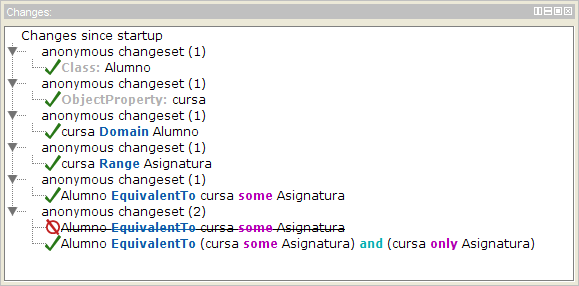
\includegraphics[width=1.00\textwidth]{Imagenes/Herramientas-changeview.png}
	\caption[ChangeView]{Vista de la herramienta ChangeView}
\end{figure}

\section{Wikis}

\subsubsection{AceWIKI}
AceWIKI\footnote{\url{http://attempto.ifi.uzh.ch/acewiki/}} Es una potente herramienta que nos permite construir una wiki sem�ntica utilizando el lenguaje ACE, lo que permite que cualquier usuario, sin tener que lidiar con RDF o OWL, pueda construir y mantener una wiki, adem�s manteniendo siempre la coherencia del contenido. 

Si bien resulta perfecta para crear cualquier ontolog�a desde cero utilizando �nicamente el lenguaje natural, no es posible la creaci�n de una wiki desde una ontolog�a dada, ya que las los individuos, clases y propiedades est�n contenidas en el propio art�culo, y no en anotaciones sobre la ontolog�a, como en otros constructores.

\subsubsection{SweetWiki}
Sweetwiki\footnote{\url{http://www-sop.inria.fr/teams/edelweiss/wiki/wakka.php?wiki=SweetWiki}} es una herramienta dise�ada para la construcci�n de wikis mediante un modelo colaborativo. Los usuarios crean y editan p�ginas y etiquetan conceptos en la wiki de manera ordinaria como en cualquier otra wiki. posteriormente, mediante herramientas facilitadas por SweetWiki, editores especializados y administradores revisan el contenido creado por los usuarios y lo complementan a�adiendo sem�ntica al contenido (mediante la inclusi�n de relaciones, por ejemplo), pero sin modificar el contenido ya creado. De este modo la navegaci�n y la b�squeda sem�ntica dentro de la wiki quedan mejoradas gracias a la sem�ntica introducida de este modo.

\subsubsection{Kaukolu}
Kaukolu\footnote{\url{http://kaukoluwiki.opendfki.de/}} es una herramienta en desarrollo que busca un enfoque alternativo para lograr mapear el contenido de una web sem�ntica a una base de conocimiento. La mayor�a de las wikis sem�nticas asocian a las p�ginas de la wiki un recurso RDF, y a los enlaces entre las p�ginas les asigna un predicado RDF. Kaukolu permite crear recursos RDF y asociarlos a fragmentos de texto formando anotaciones sobre el mismo. Una vez hecho esto, Kaukolu permite la navegaci�n por la wiki bien desde el punto de vista tradicional de las wikis, o bien a trav�s de las anotaciones creadas. 

Esta forma de trabajo resulta especialmente �til cuando queremos capturar conocimiento desde wikis corrientes, o desde textos ya creados. La captura de ese concocimiento no requiere la definici�n y utilizaci�n de sintaxis especial, ni tener que redefinir el contenido de los textos con una visi�n ```sem�ntica'' en mente, ni retocar los textos preexistentes. L�stima que la herramienta se encuentre en fase de desarrollo y no exista a�n ninguna beta del software a disposici�n del p�blico.

\subsubsection{Watson}
Watson Semantic Web Search\footnote{\url{http://watson.kmi.open.ac.uk/editor\_plugins.html}} es un proyecto que realiza labores de interfaz de acceso a la web sem�ntica. Esto se lleva a cabo recopilando contenido sem�ntico de la web, analiz�ndolo y extrayendo metainformaci�n e implementando m�todos eficaces para el acceso a la informaci�n recopilada. Todo ello permite al usuario realizar b�squedas en ontolog�as y documentos sem�nticos donde la cadena de la b�squeda aparece en identificadores, clases, propiedades, e individuos. Adem�s, permite el uso de comodines, restringir la b�squeda a ciertos tipos de entidades o a ciertos elementos de esas entidades. 
El plugin realiza la consulta en Watson Semantic Web Search\footnote{\url{http://watson.kmi.open.ac.uk/WatsonWUI/}} y nos permite, desde el propio plugin, incorporar esos resultados a la ontolog�a.

\section{Otros}

\subsubsection{BeanshellView}
BeanshellView\footnote{\url{https://code.google.com/p/co-ode-owl-plugins/wiki/BeanshellView}} es un script que permite al usuario realizar consultar o manipular la ontolog�a atrav�s del API de Prot�g� sin necesidad instalar un entorno de desarrollo java, todo ello a trav�s de un shell incrustado en Prot�g�.

\subsubsection{SWRL Tab}
SWRL Tab\footnote{\url{http://protegewiki.stanford.edu/wiki/SWRLTab}} es un plugin que nos permite la creaci�n y ejecuci�n de sentencias SWRL desde Prot�g�. Incluye una librer�a de para interactuar con documentos HTML, y bibliotecas con operadores matem�ticos, de cadenas, y RDF's. Tambi�n se incluye un lenguaje basado en OWL denominado SQWRL. Por desgracia, el plugin s�lo es compatible con las versiones 3.x de Prot�g�.

\subsubsection{Fuzzy OWL 2}
Fuzzy OWL\footnote{\url{http://nmis.isti.cnr.it/~straccia/software/FuzzyOWL/index.html}} es un plugin para Prot�g� que permite representar ontolog�as difusas, mediante el uso de anotaciones. Gracias a ello, es posible utilizar cualquier editor OWL2 (como Prot�g�) para la representaci�n de ontolog�as difusas y utilizar el razonador \textit{fuzzyDL} para responder a preguntas sobre la ontolog�a realizadas desde el propio plugin.
	



%%%% Local Variables: 
%%%% mode: latex
%%%% TeX-master: "tfc-ontologia-grado"
%%%% TeX-PDF-mode: t
%%%% ispell-local-dictionary: "castellano"
%%%% End: 

\cleardoublepage
%\chapter{Wiki Sem�nticas}

Es un error com�n el ponerse a trabajar en algo ``empezando la casa por el tejado'', es decir, sin haber sopesado las distintas opciones que tenemos a nuestro alcance, sin definir una estrategia para abordar y resolver con �xito el problema, sin utilizar herramientas adecuadas\ldots Estos pasos previos, aunque puedan suponer un coste en un primer momento, supondr�n un ahorro a la larga, puesto que estaremos eliminando desde la concepci�n de la soluci�n muchos problemas que m�s adelante supondr�n un contratiempo para el desarrollo y la implantaci�n de la soluci�n.

\section{Conclusi�n del trabajo}
A lo largo del desarrollo del proyecto, hemos visto los problemas que una soluci�n parcial, en la que se utilizan herramientas no �ptimas o inadecuadas, y donde los conceptos no est�n definidos previamente a su utilizaci�n, presenta a la hora de lidiar con un problema complejo, que incluye estructuras y conocimientos no tratados con anterioridad.

Hemos mencionado en los primeros cap�tulos los problemas de los que adolece la soluci�n ``de las hojas de c�lculo'', y hemos establecido como metas de este trabajo, principalmente, la soluci�n de esos mismos problemas. Hemos utilizado ontolog�as para definir aquellos conceptos que la reforma de la educaci�n superior ha introducido, y para fijar aquellos ya conocidos pero que por la distinta experiencia o percepci�n de cada actor \todo{Cuando hables de m�todos docentes y actividades formativas o cualquier otro concepto, aseg�rate de nombrar la fuente, hay que cambiarlo en los cap�tulos 2 y 3} presentaban matices que pueden ser objeto de controversia por su distinta interpretaci�n.

Se ha escogido un lenguaje con la expresividad suficiente como para permitir superar con �xito otro de los problemas de las hojas de c�lculo: la aplicaci�n autom�tica de aplicaciones que automaticen algunas de las tareas de inserci�n y mantenimiento del marco de conocimiento. Ahora tenemos un lenguaje computable y decidible lo que ampl�a enormemente las capacidades de la ontolog�a. �sta se ha dise�ado utilizando herramientas como Prot�g�, o HermiT, que nos han permitido asegurar la consistencia de la ontolog�a y de las instancias que de �sta se realicen, aportando la posibilidad de aplicar razonadores sobre la misma. Esta capacidad de razonamiento e inferencia nos otorga la posibilidad de realizar preguntas a la ontolog�a sobre conceptos, relaciones e individuos, de modo que una herramienta pasiva como era la hoja de c�lculo (en la que a lo sumo se podr�an hacer b�squedas, pero nada m�s complejo) se convierte en algo activo, que reacciona a nustras preguntas y que gracias a esas capacidades de inferencia y razonamiento, es capaz de mostrarnos informaci�n que no hemos introducido en la ontolog�a de manera espec�fica.

Y como colof�n, todas esas herramientas autom�ticas permiten que la ontolog�a se nos muestre de las m�s diversas formas: tabular, grafos dirigidos, nubes de tags, diagramas UML, una p�gina web, texto en varias sintaxis (RDF, Manchester,\ldots), documento java, \ldots 

Pero despu�s de eso, sigue existiendo el problema de la usabilidad. Un usuario conocedor de la materia no tendr� problemas en trabajar con grafos, o sintaxis Manchester o un diagrama UML, pero quiz�s no todo el mundo que vaya a utilizar la ontolog�a sea un experto en el manejo de Prot�g�, o sea lo suficientemente ducho en la sintaxis RDF como para lanzar consultas a la ontolog�a. Esta es una cuesti�n que deja el trabajo realizado cojo de unos de los objetivos (el m�s importante, pues si un dise�o no es usable, no habr� usuarios que trabajen con �l, y cualquier esfuerzo invertido en su desarrollo habr� sido en vano) y por ello he decidido buscar una soluci�n al problema de la usabilidad.

\section{Wikis}

\section{Wikis sem�nticas}
Las wikis sem�nticas permiten incorporar a una wiki ordinaria, un modelo de datos que permite capturar e identificar relaciones entre los diversos conceptos, de modo que es posible realizar consutas sobre el contenido y sus relaciones.



El software de wiki sem�ntica m�s extendido son Freebase, OntoWiki y Semantic Media Wiki.


Freebase consta de una colecci�n de datos estrucutrados en linea, obtenidos a partir de muy diversas fuentes, con el objetivo de crear un recurso global online que permite a los usuarios un acceso a la informaci�n eficaz y equitativo. Metaweb fue adquirida por Google en 2010. Un usuario puede realizar aportaciones a freebase, pero el esquema de datos de su aportaci�n no se adapta al com�n de la aplicaci�n hasta que un empleado de la compa�ia le da su visto bueno.

Ontowiki es una herramienta que permite la visualizaci�n de la informaci�n contenida en en una base del conocimiento, con varios puntos de vista sobre cada dato. permite la edici�n de la informaci�n de un modo simple,  y la discusi�n acerca de cada cambio realizado gracias a su control de cambios.

Semantic MediaWiki es una extensi�n de MediaWiki (herramienta para la realizaci�n de wikis sint�cticas) que permite transformar una wiki sint�ctica en una wiki sem�ntica. La principal ventaja de de SMW es la cantidad de extensiones disponibles para personalizar la wiki y a�adir nuevas utilidades.
 La principal ventaja de SMW sobre MediaWiki sobre los otros gestores de wikis es la cantidad de funcionalidades que, en forma de a�adido, se pueden utilizar para ampliar las capacidades de las wikis creadas.
 

A modo de ejemplo, se ha construido una wiki con la ontolog�a del ejemplo. Como inconveniente destacamos el hecho de que algunas estructuras sem�nticas no se puedan incorporar a la wiki (como una limitaci�n en el n�mero - al menos una- de asinaturas que componen una materia), la imposibilidad de utilizar un razonador directamente sobre la misma, y las actuaciones sobre la ontolog�a deben ser luego trasladadas a mano sobre la wiki, ya que por el momento no se ha encontrado una herramienta que realice este trasvase de informaci�n de manera autom�tica \footnote{las limitaciones sobre las estructuras sem�nticas soportadas por la wiki, hace que en ontolog�as complejas como la que estamos abordando existan construcciones que no son traducibles directamente a la wiki}, al menos con las herramientas encontradas en el directorio de extensiones de MediaWiki y Semantic MediaWiki.


Como punto a su favor, las wikis son extremadamente f�ciles de crear y mantener, y adem�s, cuentan con extensiones que facilitan la interacci�n con el usuario y protegen a la wiki de cambios que destruyan la coherencia de la informaci�n almacenada.


	\paragraph{Puesta en marcha de la wiki}
	Para poner en marcha la wiki, es preciso instalar un servidor web, php y un gestor de bases de datos. En la wiki creada al efecto hemos utilizado el software apache 2.2.22, php 5.4.6-1 y mysql 5.5.29. Sobre ello hemos puesto en marcha la versi�n 1.20 de Mediawiki y hemos instalado las extensiones SemanticMediaWiki 1.8 y Semantic Forms 2.1 para crear formularios para la introducci�n de la informaci�n por parte de los usuarios y disminuir, si no evitar, errores sem�nticos. Adicionalmente se recomienda permitir la edici�n de art�culos �nicamente a los usuarios editores y administradores.

Se han probado varias extensiones de Mediawiki y SMW que permiten subir una ontolog�a en formato RDF/XML a la wiki, como Ontology Editor o RDFIO, pero dada la complejidad de la ontolog�a, muchas de las restricciones impuestas causaban que la extensi�n fallase, o en el mejor de los casos, simplemente ignorasen esas restricciones, provocando comportamientos no deseados en la ontolog�a. Finalmente, se ha optado por crear la wiki de forma manual, al no contar con herramientas fiables que permitan el volcado de informaci�n de forma fiable, y con el fin de poder mostrar la idoneidad de trabajar con herramientas sem�nticas, como ontolog�as y wikis sem�nticas, cuando se trata de proyectos o trabajo cuyo principal objetivo es el de capturar conocimiento.
	
	
\todo{Adjuntar algunas capturas de pantalla de la wiki en el documento}
%\todo{Consideramos SPARQL �til? par apoder utilizarlo - si, inc�uyelo entre las capacidades de la wiki}

%\todo{las otras herramientas como tabajo a futro/mejoras}



%%% Local Variables: 
%%% mode: latex
%%% TeX-master: "tfc-ontologia-grado"
%%% TeX-PDF-mode: t
%%% ispell-local-dictionary: "castellano"
%%% End:
%\cleardoublepage
%\chapter{Generalizaci�n}
\todo{posibilidad: si no sacamos mucho en claro incluirlo en el capitulo de conclusiones}
hablar de las posibilidades de "portabilidad" que tiene la herramienta

\section{Intro: �qui�n puede usar esta ontolog�a? �La UCM? S�, no, pq, etc.}
hablar de a qui�n le ser�a util la ontolog�a y porqu�.

\section{Idea: jerarquia (refinamiento desde la ley hasta los planes)}
refinar el modelo hasta la ley, o explicarlo a la inversa, desde la ley.

\section{Test: Instancia UCM?}
hacer pruebas con otras instancias.

%%% Local Variables: 
%%% mode: latex
%%% TeX-master: "tfc-ontologia-grado"
%%% TeX-PDF-mode: t
%%% ispell-local-dictionary: "castellano"
%%% End: 

%\cleardoublepage
%\chapter{Conclusiones}

%%% Local Variables: 
%%% mode: latex
%%% TeX-master: "tfc-ontologia-grado"
%%% TeX-PDF-mode: t
%%% ispell-local-dictionary: "castellano"
%%% End: 

%\cleardoublepage

%%%%%%%%%%%%%%%%%%%%%%%%%%%%%%%%%%%%%%%%%%%%%%%%%%%%%%%%%%%%%%%%%%%%%%
%% COMIENZO DE LOS APÉNDICES
%% (NO TOCAR)
\appendix

%%%%%%%%%%%%%%%%%%%%%%%%%%%%%%%%%%%%%%%%%%%%%%%%%%%%%%%%%%%%%%%%%%%%%%
%% APÉNDICES:
%%  * PONER CADA APÉNDICE EN UN FICHERO COMO SI FUERAN CAPÍTULOS
%%  * HACER UN include POR CADA FICHERO E INCLUIRLO EN includeonly
%%  * AÑADIR \clearemptydoublepage DESPUÉS DE CADA include
%%
%%
%% Semántica de Manchester
%\chapter{Sem�ntica de Manchester}

\section{Vocabulario}

\lstset{language=owlms,numbers=none,literate=,mathescape,backgroundcolor=}

El mapa de los tipos de datos es una sextupla de la forma: \newline
\begin{center}
$D=(N_{DT}, N_{LS}, N_{FS}, \cdot^{DT},\cdot^{LS},\cdot^{FS})$
\end{center}
donde:
\begin{itemize}
	\item $N_{DT}$ es un conjunto de tipos de datos donde no est� incluido el tipo $rdfs:Literal$.
	\item $N_{LS}$ es una funci�n que asigna a cada tipo de datos $DT \in N_{DT}$ un conjunto $N_{LS}(DT)$ de strings llamados \textit{formas l�xicas}. El conjunto $N_{LS}(DT)$ recibe el nombre de \textit{espacio l�xico} de DT.
	\item $N_{FS}$ es una funci�n que asigna a cada tipo de datos $DT \in N_{DT}$ un conjunto $N_{FS}(DT)$ de pares $(F, v)$, donde $F$ es una \textit{dimensi�n restringida} y $v$ es un valor arbitrario llamado \textit{valor restringido}. El conjunto $N_{FS}(DT)$ se llama \textit{espacio de dimensiones} de $DT$.
	\item Para cada tipo de datos $DT \in N_{DT}$, la \textit{funci�n de interpretaci�n} $\cdot^{DT}$ asigna a $DT$ un conjunto $(DT)^{DT}$ llamado \textit{espacio de valores} de $DT$.
	\item Para cada tipo de datos $DT \in N_{DT}$ y cada forma l�xica $LV \in N_{LS}(DT)$, la \textit{funci�n de interpretaci�n} $\cdot^{LS}$ asigna al par $(LV, DT)$ el valor $(LV, DT)^{LS} \in (DT)^{DT}$.
	\item Para cada tipo de datos $DT \in N_{DT}$ y cada par $(F, v) \in N_{FS}(DT)$, la \textit{funci�n de interpretaci�n} $\cdot^{FS}$ asigna a $(F, v)$ el conjunto $(F, v)^{FS} \subseteq (DT)^{DT}$.
\end{itemize}
%
Un vocabulario $V=(V_C, V_{OP}, V_{DP}, V_I, V_{DT}, V_{LT}, V_{FA})$ sobre un mapa de datos $D$ es una s�ptupla que consta de los siguientes elementos:
\begin{itemize}
	\item $V_C$ es un conjunto de clases seg�n la especificaci�n \textit{OWL2}\footnote{http://www.w3.org/TR/owl2-direct-semantics/\#ref-owl-2-specification} que contiene al menos las clases \textit{owl:Thing} y \textit{owl:Nothing}.
	\item $V_{OP}$ es un conjunto de propiedades sobre objetos tal y como est�n definidos en la especificaci�n \textit{OWL2}, que contiene al menos las propiedades \textit{owl:topObjectPropertiy} y \textit{owl:bottomObjectProperty}.
	\item $V_{DP}$ es un conjunto de propiedades de datos seg�n la especificaci�n \textit{OWL2} que contiene al menos las propiedades \textit{owl:topDataProperty} y \textit{owl:bottomDataProperty}.
	\item $V_I$ es un conjunto de individuos (con nombre y an�nimos) tal y como se definen en la especificaci�n de \textit{OWL2}
	\item $V_{DT}$ es el conjunto que contiene todos los tipos de datos definidos en $D$, el tipo de datos \textit{rdfs:Literal}, y posiblemente otros tipos de datos, lo que nos lleva a inferir que $N_{DT} \cup \{ rdfs:Literal \} \subseteq V_{DT}$.
	\item $V_{LT}$ es un conjunto de literales $(LV)^{DT}$ para cada tipo de datos $DT \in N_{DT}$ y cada forma l�xica $LV \in N_{LS}(DT)$.
	\item $V_{FA}$ es el conjunto de pares $(F, lt)$ para cada dimensi�n restringida $F$, tipo de datos $DT \in N_{DT}$ y literal $lt \in V_{LT}$ tales que $(F, (LV, DT_1)^{LS}) \in N_{FS}(DT)$, donde $LV$ es la forma l�xica de $lt$ y $DT_1$ es el tipo de datos de $lt$.
\end{itemize}

Dado un vocabulario $V$, de ahora en adelante se utilizar� la siguiente notac��n:
\begin{itemize}
	\item $OP$ denota una propiedad de un objeto.
	\item $OPE$ denota una expresi�n de una propiedad de un objeto.
	\item $DP$ denota una propiedad de un dato.
	\item $DPE$ denota una expresi�n de una propiedad de un dato.
	\item $C$ denota una clase.
	\item $CE$ denota una expresi�n de una clase.
	\item $DT$ denota un tipo de datos.
	\item $DR$ denota un rango de datos.
	\item $a$ denota un individuo, con nombre o an�nimo.
	\item $lt$ denota un literal.
	\item $F$ denota una dimensi�n restringida.
\end{itemize}

\section{Interpretaci�n}
	Dado un mapa de tipos de datos $D$, y un vocabulario $V$ sobre $D$, una interpretaci�n $I=(\bigtriangleup_I, \bigtriangleup_D, \cdot^C, \cdot^{OP}, \cdot^{DP}, \cdot^I, \cdot^{DT}, \cdot^{LT}, \cdot^{FA})$ para $D$ y $V$ es una 9-tupla con la siguiente estructura:
	\begin{itemize}
		\item $\bigtriangleup_I$ es un conjunto no vac�o llamado el \textit{dominio de objetos}.
		\item $\bigtriangleup_D$ es un conjunto no vac�o disjunto a $\bigtriangleup_I$ llamado el \textit{dominio de datos} tal que $(DT)^{DT} \subseteq \bigtriangleup_D$ para cada tipo de datos $DT \in V_{DT}$.
		\item $\cdot^C$ es la \textit{funci�n de intrepretaci�n de clases} que asigna a cada clase $C \in V_C$ un subconjunto $(C)^C \subseteq \bigtriangleup_I$ tal que $(owl_Thing)^C=\bigtriangleup_I \cap (owl:Thing)^C=\varnothing$.
		\item $\cdot^{OP}$ es la \textit{funci�n de interpretaci�n de propiedades de objetos} que asigna a cada propiedad $OP \in V_{OP}$ un subconjunto $(OP)^{OP} \subseteq \bigtriangleup_I \times \bigtriangleup_I$ tal que $(owl:topObjectProperty)^{OP}=\bigtriangleup_I \times \bigtriangleup_I \land (owl:bottomObjectProperty)^{OP}=\varnothing$.
		\item $\cdot^{DP}$ es la \textit{funci�n de interpretaci�n de datos} que asigna a cada propiedad $DP \in V_{DP}$ un subconjunto $(DP)^{DP} \subseteq \bigtriangleup_I \times \bigtriangleup_D$ tal que $(owl:topDataProperty)^{DP}=\bigtriangleup_I \times \bigtriangleup_D \land (owl:bottomDataProperty)^{DP}=\varnothing$.
		\item $\cdot^I$ es la \textit{funci�n de interpretaci�n de individuos} que asigna a cada individuo $a \in V_I$ un elemento $(a)^I \in \bigtriangleup_I$.
		\item $\cdot^{DT}$ es la funci�n de interpretaci�n de tipos de datos que asigna a cada tipo de datos $DT \in V_{DT}$ un subconjunto $(DT)^{DT} \subseteq \bigtriangleup_D$ tal que $\cdot^{DT}$ es igual que en D para cada tipo de datos $DT \in N_{DT} \land (rdfs:Literal)^{DT} = \bigtriangleup_D$.
		\item $\cdot^{LT}$ es la \textit{funci�n de interpretaci�n literal} que se define como $(lt)^{LT}=(LV,, DT)^{LS}$ para cada $lt \in V_{LT}$, donde $LV$ es la forma l�xica de $lt$ y $DT$ es el tipo de datos de $lt$.
		\item $\cdot^{FA}$ es la \textit{funci�n de interpretaci�n de dimensiones} que se define como $(F, lt)^{FA}=(F,(lt)^{LT})^{FS}$ para cada $(F, lt) \in V_{FA}$.
	\end{itemize}

\section{Satisfacci�n de axiomas}

\begin{center}
	\begin{longtable}{||p{0.45\linewidth}|p{0.55\linewidth}||}
		\hline
		\hline
		\multicolumn{2}{||c||}{Satisfacci�n de axiomas sobre clases:}\\
		\hline
		Axioma & Condici�n\\
		\hline
		\endhead
		%%%%%%%%%%%%%%%%%%%%%%%%%%%%%%%%%%%%%%%%%%%
		%% Class: A SubClassOf B %%%%%%%%%%%%%%%%%%
		%%%%%%%%%%%%%%%%%%%%%%%%%%%%%%%%%%%%%%%%%%%
		\begin{lstlisting}[nolol=true]
Class: $CE$
  SubClassOf: $CE_1,\dotsc,CE_n$
    \end{lstlisting}
    &
    \begin{displaymath}
      \begin{array}{l}
        (CE)^c\subseteq(CE_1)^c \cap \dotsb \cap (CE)^c\subseteq(CE_n)^c\\
      \end{array}
    \end{displaymath}
    \\
    \hline
		%%%%%%%%%%%%%%%%%%%%%%%%%%%%%%%%%%%%%%%%%%%
		%% Class: A EquivalentOf B %%%%%%%%%%%%%%%%
		%%%%%%%%%%%%%%%%%%%%%%%%%%%%%%%%%%%%%%%%%%%
		\begin{lstlisting}[nolol=true]
Class: $CE_1$ 
   EquivalentTo: $CE_2,\dotsc,CE_n$
    \end{lstlisting}
    &
    \begin{displaymath}
    	\begin{array}{l}
   		   (CE_j)^c = (CE_k)^c \\
   		   \text{ para cada } 1 \leq j \leq n, 1 \leq j \leq n\\
   		\end{array}
   	\end{displaymath}
   	\\
   	\hline
   	%%%%%%%%%%%%%%%%%%%%%%%%%%%%%%%%%%%%%%%%%%%  
   	%% Class: A DisjointWith B %%%%%%%%%%%%%%%%
		%%%%%%%%%%%%%%%%%%%%%%%%%%%%%%%%%%%%%%%%%%%
		\begin{lstlisting}[nolol=true]
Class: $CE_1$
	DisjointWith: $CE_2,\dotsc,CE_n$
    \end{lstlisting}
    &
    \begin{displaymath}
    	\begin{array}{l}
   		   (CE_j)^c \cap (CE_k)^c = \varnothing \\
   		   \text{ para cada } 1 \leq j \leq n, 1 \leq k \leq n \\
   		   \text{ tales que } j \neq k\\
   		\end{array}
   	\end{displaymath}
   	\\ 
    \hline
   	%%%%%%%%%%%%%%%%%%%%%%%%%%%%%%%%%%%%%%%%%%%  
   	%% Class: A DisjointUnionOf B %%%%%%%%%%%%%
		%%%%%%%%%%%%%%%%%%%%%%%%%%%%%%%%%%%%%%%%%%%
		\begin{lstlisting}[nolol=true]
Class: $CE$
  DisjointUnionOf: $CE_1,\dotsc,CE_n$
    \end{lstlisting}
    &
    \begin{displaymath}
      \begin{array}{l}
        CE^c=(CE_1)^c \cup \dotsc \cup (CE_n)^c \\
        \land \\
        (CE_j)^c \cap (CE_k)^c = \varnothing \\
        \text{ para cada } 1\leq j \leq  n, 1 \leq k \leq  n \\
        \text{ tales que } j \neq k\\
   		\end{array}
   	\end{displaymath}
   	\\ 
   	\hline
   	%%%%%%%%%%%%%%%%%%%%%%%%%%%%%%%%%  
   	%% DisjointClasses  %%%%%%%%%%%%%
	%%%%%%%%%%%%%%%%%%%%%%%%%%%%%%%%%
		\begin{lstlisting}[nolol=true]
DisjointClasses: $CE_1,\dotsc,CE_n$
    \end{lstlisting}
    &
    \begin{displaymath}
      \begin{array}{l}
        (CE_j)^c \cap (CE_k)^c = \varnothing \\
        \text{ para cada } 1\leq j \leq  n \text{, } j < k \leq  n \\
   		\end{array}
   	\end{displaymath}
   	\\ 
   	\hline
   	\hline
   	\end{longtable}
\end{center}

\begin{center}
	\begin{longtable}{||p{0.45\linewidth}|p{0.55\linewidth}||}
		\hline
		\hline
		\multicolumn{2}{||c||}{Satisfacci�n de axiomas sobre propiedades de objetos:}\\
		\hline
		Axioma & Condici�n\\
		\hline
		\endhead
   	%%%%%%%%%%%%%%%%%%%%%%%%%%%%%%%%%%%%%%%%%%%  
   	%% SubPropertyOf %%%%%%%%%%%%%%%%%%%%%%%%%%
		%%%%%%%%%%%%%%%%%%%%%%%%%%%%%%%%%%%%%%%%%%%
		\begin{lstlisting}[nolol=true]
ObjectProperty: $OPE_1$
	SubPropertyOf: $OPE_2$
    \end{lstlisting}
    &
    \begin{displaymath}
    	\begin{array}{l}
   		  (OPE_1)^{op} \subseteq (OPE_2)^{op}\\
   		\end{array}
   	\end{displaymath}
   	\\ 
   	\hline
   	%%%%%%%%%%%%%%%%%%%%%%%%%%%%%%%%%%%%%%%%%%%  
   	%% SubPropertyChain %%%%%%%%%%%%%%%%%%%%%%%
		%%%%%%%%%%%%%%%%%%%%%%%%%%%%%%%%%%%%%%%%%%%
		\begin{lstlisting}[nolol=true]
ObjectProperty: $OPE$
	SubPropertyChain: $OPE_1, \dotsc, OPE_n$
    \end{lstlisting}
    &
    \begin{displaymath}
    	\begin{array}{l}
   		  \forall y_0 \ldots Y_n:(y_0,y_1) \in (OPE_1)^{op} \\
   		  	\text{ and } \ldots \text{ and } \\
   		  	(y_{n-1}, y_n) \in (OPE_n)^{op} \Rightarrow (y_0, y_n) \in (OPE)^{op}\\
   		\end{array}
   	\end{displaymath}
   	\\ 
   	\hline
   	%%%%%%%%%%%%%%%%%%%%%%%%%%%%%%%%%%%%%%%%%%%  
   	%% ObjectProperty: A Domain B %%%%%%%%%%%%%
		%%%%%%%%%%%%%%%%%%%%%%%%%%%%%%%%%%%%%%%%%%%
		\begin{lstlisting}[nolol=true]
ObjectProperty: $OPE$
	Domain: $CE$
    \end{lstlisting}
    &
    \begin{displaymath}
    	\begin{array}{l}
   		  \forall x,y:(x,y) \in (OPE)^{op} \Rightarrow x \in (CE)^c\\
   		\end{array}
   	\end{displaymath}
   	\\ 
   	\hline
   	%%%%%%%%%%%%%%%%%%%%%%%%%%%%%%%%%%%%%%%%%%%  
   	%% ObjectProperty: A Range B %%%%%%%%%%%%%%
		%%%%%%%%%%%%%%%%%%%%%%%%%%%%%%%%%%%%%%%%%%%
		\begin{lstlisting}[nolol=true]
ObjectProperty: $OPE$
	Range: $CE$
    \end{lstlisting}
    &
    \begin{displaymath}
    	\begin{array}{l}
    		\forall x,y:(x,y) \in (OPE)^{op} \Rightarrow y \in (CE)^c\\
   		\end{array}
   	\end{displaymath}
   	\\ 
   	\hline
   	%%%%%%%%%%%%%%%%%%%%%%%%%%%%%%%%%%%%%%%%%%%%%%%%%%%%%%  
   	%% ObjectProperty: A Characteristics:Functional %%%%%%
		%%%%%%%%%%%%%%%%%%%%%%%%%%%%%%%%%%%%%%%%%%%%%%%%%%%%%%
		\begin{lstlisting}[nolol=true]
ObjectProperty: $OPE$
	Characteristics: Functional
    \end{lstlisting}
    &
    \begin{displaymath}
    	\begin{array}{l}
   		   \forall x,y_1,y_2:(x,y_1) \in (OPE)^{op}\\
   		   \land\\
   		   (x,y_2) \in (OPE)^{op}	 \Rightarrow  y_1=y_2\\
   		\end{array}
   	\end{displaymath}
   	\\ 
    \hline
   	%%%%%%%%%%%%%%%%%%%%%%%%%%%%%%%%%%%%%%%%%%%%%%%%%%%%%%%%%%%%%  
   	%% ObjectProperty: A Characteristcs: InverseFunctional %%%%%%
		%%%%%%%%%%%%%%%%%%%%%%%%%%%%%%%%%%%%%%%%%%%%%%%%%%%%%%%%%%%%%
		\begin{lstlisting}[nolol=true]
ObjectProperty: $OPE$
	Characteristics: InverseFunctional
    \end{lstlisting}
    &
    \begin{displaymath}
    	\begin{array}{l}
   		   \forall x_1,x_2,y:(x_1,y)\in (OPE)^{op}\\
   		   \land \\
   		   (x_2,y) \in (OPE)^{op} \Rightarrow x_1=x_2\\
   		\end{array}
   	\end{displaymath}
   	\\
    \hline 
   	%%%%%%%%%%%%%%%%%%%%%%%%%%%%%%%%%%%%%%%%%%%%%%%%%%%%%%  
   	%% ObjectProperty: A Characteristics: Reflexive %%%%%%
		%%%%%%%%%%%%%%%%%%%%%%%%%%%%%%%%%%%%%%%%%%%%%%%%%%%%%%
		\begin{lstlisting}[nolol=true]
ObjectProperty: $OPE$
	Characteristics: Reflexive
    \end{lstlisting}
    &
    \begin{displaymath}
    	\begin{array}{l}
   		   \forall x:x\in \bigtriangleup_I \Rightarrow (x,x) \in (OPE)^{op}\\\\
   		\end{array}
   	\end{displaymath}
   	\\
    \hline 
   	%%%%%%%%%%%%%%%%%%%%%%%%%%%%%%%%%%%%%%%%%%%%%%%%%%%%%%%%  
   	%% ObjectProperty: A Characteristics: Irreflexive %%%%%%
		%%%%%%%%%%%%%%%%%%%%%%%%%%%%%%%%%%%%%%%%%%%%%%%%%%%%%%%%
		\begin{lstlisting}[nolol=true]
ObjectProperty: $OPE$
	Characteristics: Irreflexive
    \end{lstlisting}
    &
    \begin{displaymath}
    	\begin{array}{l}
   		   \forall x:x \in \bigtriangleup_I \Rightarrow (x,x) \notin (OPE)^{op}\\\\
   		\end{array}
   	\end{displaymath}
   	\\
    \hline 
   	%%%%%%%%%%%%%%%%%%%%%%%%%%%%%%%%%%%%%%%%%%%%%%%%%%%%%%  
   	%% ObjectProperty: A Characteristics: Symmetric %%%%%%
		%%%%%%%%%%%%%%%%%%%%%%%%%%%%%%%%%%%%%%%%%%%%%%%%%%%%%%
		\begin{lstlisting}[nolol=true]
ObjectProperty: $OPE$
	Charactetistics: Symmetric
    \end{lstlisting}
    &
    \begin{displaymath}
    	\begin{array}{l}
   		   \forall x,y:(x,y) \in (OPE)^{op} \Rightarrow (y,x)\in (OPE)^{op}\\\\
   		\end{array}
   	\end{displaymath}
   	\\
    \hline 
   	%%%%%%%%%%%%%%%%%%%%%%%%%%%%%%%%%%%%%%%%%%%%%%%%%%%%%%%  
   	%% ObjectProperty: A Charactetistics: Asymmetric %%%%%%
		%%%%%%%%%%%%%%%%%%%%%%%%%%%%%%%%%%%%%%%%%%%%%%%%%%%%%%%
		\begin{lstlisting}[nolol=true]
ObjectProperty: $OPE$
	Characteristics: Asymmetric
    \end{lstlisting}
    &
    \begin{displaymath}
    	\begin{array}{l}
   		   \forall x,y:(x,y) \in (OPE)^{op} \Rightarrow (y,x)\notin (OPE)^{op}\\\
   		\end{array}
   	\end{displaymath}
   	\\
    \hline 
   	%%%%%%%%%%%%%%%%%%%%%%%%%%%%%%%%%%%%%%%%%%%%%%%%%%%%%%%  
   	%% ObjectProperty: A Characteristics: Transitive %%%%%%
		%%%%%%%%%%%%%%%%%%%%%%%%%%%%%%%%%%%%%%%%%%%%%%%%%%%%%%%
		\begin{lstlisting}[nolol=true]
ObjectProperty: $OPE$
	Characteristics: Transitive
    \end{lstlisting}
    &
    \begin{displaymath}
    	\begin{array}{l}
   		   \forall x,y,z:(x,y) \in (OPE)^op \\
   		   \land \\
   		   y,z) \in (OPE)^{op} \Rightarrow (x,z) \in (OPE)^{op}\\
   		\end{array}
   	\end{displaymath}
   	\\
    \hline 
   	%%%%%%%%%%%%%%%%%%%%%%%%%%%%%%%%%%%%%%%%%%%  
   	%% ObjectProperty: A SubPropertyOf B %%%%%%
		%%%%%%%%%%%%%%%%%%%%%%%%%%%%%%%%%%%%%%%%%%%
		\begin{lstlisting}[nolol=true]
ObjectProperty: $OPE_1$
	SubPropertyOf: $OPE_2$
    \end{lstlisting}
    &
    \begin{displaymath}
    	\begin{array}{l}
   		   (OPE_1)^{op} \subseteq (OPE_2)^{op}\\
   		\end{array}
   	\end{displaymath}
   	\\
    \hline 
   	%%%%%%%%%%%%%%%%%%%%%%%%%%%%%%%%%%%%%%%%%%%  
   	%% ObjectProperty: A EquivalentTo B %%%%%%
		%%%%%%%%%%%%%%%%%%%%%%%%%%%%%%%%%%%%%%%%%%%
		\begin{lstlisting}[nolol=true]
ObjectProperty: $OPE_1$
	EquivalentTo: $OPE_2,\dotsc,OPE_n$
    \end{lstlisting}
    &
    \begin{displaymath}
    	\begin{array}{l}
   		   (OPE_j)^{op}=(OPE_k)^{op} \\
   		   \text{para cada } 1 \leq j \leq n \text{ y cada } 1 \leq k \leq n\\
   		\end{array}
   	\end{displaymath}
   	\\
    \hline
   	%%%%%%%%%%%%%%%%%%%%%%%%%%%%%%%%%%%%%%%%%%  
   	%% ObjectProperty: A DisjointWith B %%%%%%
		%%%%%%%%%%%%%%%%%%%%%%%%%%%%%%%%%%%%%%%%%%
		\begin{lstlisting}[nolol=true]
ObjectProperty: $OPE_1$
	DisjointWith: $OPE_2,\dotsc,OPE_n$
    \end{lstlisting}
    &
    \begin{displaymath}
    	\begin{array}{l}
   		   (OPE_j)^{op} \cap (OPE_k)^{op} = \varnothing \\
   		   \text{para cada } 1 \leq j \leq n \text{ y cada } 1 \leq k \leq n\\
   		   \text{tales que } j \neq k
   		\end{array}
   	\end{displaymath}
   	\\
    \hline  
   	%%%%%%%%%%%%%%%%%%%%%%%%%%%%%%%%%%%%%%%%%%%  
   	%% ObjectProperty: A InverseOf B %%%%%%%%%%
		%%%%%%%%%%%%%%%%%%%%%%%%%%%%%%%%%%%%%%%%%%%
		\begin{lstlisting}[nolol=true]
ObjectProperty: $OPE_1$
	InverseOf: $OPE_2$
    \end{lstlisting}
    &
    \begin{displaymath}
    	\begin{array}{l}
   		  (OPE_1)^{op} = \{(x,y) \vert (y,x) \in (OPE_2)^{op}\}\\
   		\end{array}
   	\end{displaymath}
   	\\
    \hline 
    \hline
	\end{longtable}
\end{center}

\begin{center}
	\begin{longtable}{||p{0.45\linewidth}|p{0.55\linewidth}||}
		\hline
		\hline
		\multicolumn{2}{||c||}{Satisfacci�n de axiomas sobre datos:}\\
		\hline
		Axioma & Condici�n\\
		\hline
		\endhead
   	%%%%%%%%%%%%%%%%%%%%%%%%%%%%%%%%%%%%%%%%%%%  
   	%% DataProperty: A Domain B %%%%%%%%%%%%%%%
		%%%%%%%%%%%%%%%%%%%%%%%%%%%%%%%%%%%%%%%%%%%
		\begin{lstlisting}[nolol=true]
DataProperty: $DPE$
	Domain: $CE$
    \end{lstlisting}
    &
    \begin{displaymath}
    	\begin{array}{l}
   		   \forall x,y:(x,y) \in (DPE)^{dp} \Rightarrow x \in (CE)^{c}\\
   		\end{array}
   	\end{displaymath}
   	\\
    \hline 
   	%%%%%%%%%%%%%%%%%%%%%%%%%%%%%%%%%%%%%%%%%%%  
   	%% DataProperty: A Range B %%%%%%%%%%%%%%%%
		%%%%%%%%%%%%%%%%%%%%%%%%%%%%%%%%%%%%%%%%%%%
		\begin{lstlisting}[nolol=true]
DataProperty: $DPE_1$
	Range: $DR$
    \end{lstlisting}
    &
    \begin{displaymath}
    	\begin{array}{l}
   		   \forall x,y(x,y) \in (DPE)^{dp} \Rightarrow y \in (DR)^{dt}\\
   		\end{array}
   	\end{displaymath}
   	\\
    \hline 
   	%%%%%%%%%%%%%%%%%%%%%%%%%%%%%%%%%%%%%%%%%%%%%%%%%%%%  
   	%% DataProperty: A Characteristics Functional %%%%%%
		%%%%%%%%%%%%%%%%%%%%%%%%%%%%%%%%%%%%%%%%%%%%%%%%%%%%
		\begin{lstlisting}[nolol=true]
DataProperty: $DPE$
	Characteristics: Functional
    \end{lstlisting}
    &
    \begin{displaymath}
    	\begin{array}{l}
    		\forall x,y_1,y_2:(x,y_1)\in (DPE)^{dp}\\
				\land\\	
				(x,y_2)\in (DPE)^{dp} \Rightarrow y_1=y_2\\
   		\end{array}
   	\end{displaymath}
   	\\
    \hline
   	%%%%%%%%%%%%%%%%%%%%%%%%%%%%%%%%%%%%%%%%%%%  
   	%% DataProperty: A SubPropertyOf B %%%%%%
		%%%%%%%%%%%%%%%%%%%%%%%%%%%%%%%%%%%%%%%%%%%
		\begin{lstlisting}[nolol=true]
DataProperty: $DPE_1$
	SubPropertyOf: $DPE_2$
    \end{lstlisting}
    &
    \begin{displaymath}
    	\begin{array}{l}
   		   (DPE_1)^{dp} \subseteq (DPE_2)^{dp}\\
   		\end{array}
   	\end{displaymath}
   	\\
    \hline  
   	%%%%%%%%%%%%%%%%%%%%%%%%%%%%%%%%%%%%%%%%%%%  
   	%% DataProperty: A EquivalentTo B %%%%%%
		%%%%%%%%%%%%%%%%%%%%%%%%%%%%%%%%%%%%%%%%%%%
		\begin{lstlisting}[nolol=true]
DataProperty: $DPE_1$
	EquivalentTo: $DPE_2,\dotsc,DPE_n$
    \end{lstlisting}
    &
    \begin{displaymath}
    	\begin{array}{l}
   		   (DPE_j)^{dp}=(DPE_k)^{dp}\\
   		   \text{ para cada } 1 \leq j \leq n \\
   		   \text{ y cada } 1 \leq k \leq n\\
   		\end{array}
   	\end{displaymath}
   	\\
    \hline 
   	%%%%%%%%%%%%%%%%%%%%%%%%%%%%%%%%%%%%%%%%%%%  
   	%% DataProperty: A DisjointWith B %%%%%%
		%%%%%%%%%%%%%%%%%%%%%%%%%%%%%%%%%%%%%%%%%%%
		\begin{lstlisting}[nolol=true]
DataProperty: $DPE_1$
	DisjointWith: $DPE_2,\dotsc,DPE_n$
    \end{lstlisting}
    &
    \begin{displaymath}
    	\begin{array}{l}
   		   (DPE_j)^{dp} \cap (DPE_k)^{dp} = \varnothing \\
   		   	\text{para cada} 1 \leq j \leq n \\
   		   \text{y cada } 1 \leq k \leq n 
   		   \text{tales que } j \neq k\\
   		\end{array}
   	\end{displaymath}
   	\\
    \hline 
	\end{longtable}
\end{center}

\begin{center}
	\begin{longtable}{||p{0.45\linewidth}|p{0.55\linewidth}||}
		\hline
		\hline
		\multicolumn{2}{||c||}{Expresiones:}\\
		\hline
		Expresi�n & Interpretaci�n\\
		\hline
		\endhead
   	%%%%%%%%%%%%%%%%%%%%%%%%%%%%%%%%%%%%%%%%%%%  
   	%% A and B %%%%%%%%%%%%%%%%%%%%%%%%%%%%%%%%
		%%%%%%%%%%%%%%%%%%%%%%%%%%%%%%%%%%%%%%%%%%%
		\begin{lstlisting}[nolol=true]
$CE_1$ and $\dotsc$ and $CE_n$
    \end{lstlisting}
    &
    \begin{displaymath}
    	\begin{array}{l}
   		  (CE_1)^c \cap \dotsc \cap (CE_n)^c\\
   		\end{array}
   	\end{displaymath}
   	\\ 
   	\hline
   	%%%%%%%%%%%%%%%%%%%%%%%%%%%%%%%%%%%%%%%%%%%  
   	%% A or B %%%%%%%%%%%%%%%%%%%%%%%%%%%%%%%%%
		%%%%%%%%%%%%%%%%%%%%%%%%%%%%%%%%%%%%%%%%%%%
		\begin{lstlisting}[nolol=true]
$CE_1$ or $\dotsc$ or $CE_n$
    \end{lstlisting}
    &
    \begin{displaymath}
    	\begin{array}{l}
   		  (CE_1)^c \cup \dotsc \cup (CE_n)^c\\
   		\end{array}
   	\end{displaymath}
   	\\ 
   	\hline  
   	%%%%%%%%%%%%%%%%%%%%%%%%%%%%%%%%%%%%%%%%%%%  
   	%% NOT A %%%%%%%%%%%%%%%%%%%%%%%%%%%%%%%%%%
		%%%%%%%%%%%%%%%%%%%%%%%%%%%%%%%%%%%%%%%%%%%
		\begin{lstlisting}[nolol=true]
not $CE$
    \end{lstlisting}
    &
    \begin{displaymath}
    	\begin{array}{l}
   		  \bigtriangleup_I \backslash (CE)^c \\
   		\end{array}
   	\end{displaymath}
   	\\ 
   	\hline  
   	%%%%%%%%%%%%%%%%%%%%%%%%%%%%%%%%%%%%%%%%%%%  
   	%% {a, b} %%%%%%%%%%%%%
		%%%%%%%%%%%%%%%%%%%%%%%%%%%%%%%%%%%%%%%%%%%
		\begin{lstlisting}[nolol=true]
{$a_1$, $\dotsc$, $a_n$}
    \end{lstlisting}
    &
    \begin{displaymath}
    	\begin{array}{l}
   		  \{(a_1)^I, \dotsc, (a_n)^I\}\\
   		\end{array}
   	\end{displaymath}
   	\\ 
   	\hline  
   	%%%%%%%%%%%%%%%%%%%%%%%%%%%%%%%%%%%%%%%%%%%  
   	%% M some A %%%%%%%%%%%%%
		%%%%%%%%%%%%%%%%%%%%%%%%%%%%%%%%%%%%%%%%%%%
		\begin{lstlisting}[nolol=true]
$OPE$ some $CE$
    \end{lstlisting}
    &
    \begin{displaymath}
    	\begin{array}{l}
   		  \{x| \exists y:(x,y) \in (OPE)^{op} \land y \in (CE)^c\}
   		\end{array}
   	\end{displaymath}
   	\\ 
   	\hline  
   	%%%%%%%%%%%%%%%%%%%%%%%%%%%%%%%%%%%%%%%%%%%  
   	%% M only A %%%%%%%%%%%%%
		%%%%%%%%%%%%%%%%%%%%%%%%%%%%%%%%%%%%%%%%%%%
		\begin{lstlisting}[nolol=true]
$OPE$ only $CE$
    \end{lstlisting}
    &
    \begin{displaymath}
    	\begin{array}{l}
   		  \{x| \forall y:(x,y) \in (OPE)^{op} \implies y \in (CE)^c\}\\
   		\end{array}
   	\end{displaymath}
   	\\ 
   	\hline  
    %%%%%%%%%%%%%%%%%%%%%%%%%%%%%%%%%%%%%%%%%%%  
   	%% M has value a %%%%%%%%%%%%%
		%%%%%%%%%%%%%%%%%%%%%%%%%%%%%%%%%%%%%%%%%%%
		\begin{lstlisting}[nolol=true]
$OPE$ value $a$
    \end{lstlisting}
    &
    \begin{displaymath}
    	\begin{array}{l}
   		  \{x| (x,(a)^I) \in (OPE)^{op}\}\\
   		\end{array}
   	\end{displaymath}
   	\\ 
   	\hline  
   	%%%%%%%%%%%%%%%%%%%%%%%%%%%%%%%%%%%%%%%%%%%  
   	%% M self %%%%%%%%%%%%%
		%%%%%%%%%%%%%%%%%%%%%%%%%%%%%%%%%%%%%%%%%%%
		\begin{lstlisting}[nolol=true]
$OPE$ self
    \end{lstlisting}
    &
    \begin{displaymath}
    	\begin{array}{l}
   		  \{x| (x,x) \in (OPE)^{op}\}\\
   		\end{array}
   	\end{displaymath}
   	\\ 
   	\hline
		%%%%%%%%%%%%%%%%%%%%%%%%%%%%%%%%%%%%%%%%%%%  
   	%% M min n %%%%%%%%%%%%%
		%%%%%%%%%%%%%%%%%%%%%%%%%%%%%%%%%%%%%%%%%%%
		\begin{lstlisting}[nolol=true]
$OPE$ min $n$
    \end{lstlisting}
    &
    \begin{displaymath}
    	\begin{array}{l}
   		  \{x|\ \#\ \{y|(x,y)\in(OPE)^{OP}\} \geq n \} \\
   		\end{array}
   	\end{displaymath}
   	\\ 
   	\hline     	  
		%%%%%%%%%%%%%%%%%%%%%%%%%%%%%%%%%%%%%%%%%%%  
   	%% M max n %%%%%%%%%%%%%
		%%%%%%%%%%%%%%%%%%%%%%%%%%%%%%%%%%%%%%%%%%%
		\begin{lstlisting}[nolol=true]
$OPE$ max $n$
    \end{lstlisting}
    &
    \begin{displaymath}
    	\begin{array}{l}
   		  \{x|\ \#\ \{y|(x,y)\in(OPE)^{OP}\} \leq n \} \\
   		\end{array}
   	\end{displaymath}
   	\\ 
   	\hline 
		%%%%%%%%%%%%%%%%%%%%%%%%%%%%%%%%%%%%%%%%%%%  
   	%% M exactly n %%%%%%%%%%%%%
		%%%%%%%%%%%%%%%%%%%%%%%%%%%%%%%%%%%%%%%%%%%
		\begin{lstlisting}[nolol=true]
$OPE$ exactly $n$
    \end{lstlisting}
    &
    \begin{displaymath}
    	\begin{array}{l}
   		  \{x|\ \#\ \{y|(x,y)\in(OPE)^{OP}\} = n \} \\
   		\end{array}
   	\end{displaymath}
   	\\ 
   	\hline     	  
		%%%%%%%%%%%%%%%%%%%%%%%%%%%%%%%%%%%%%%%%%%%  
   	%% P some n %%%%%%%%%%%%%%%%%%%%%%%%%%%%%%%
		%%%%%%%%%%%%%%%%%%%%%%%%%%%%%%%%%%%%%%%%%%%
		\begin{lstlisting}[nolol=true]
$DPE$ some $DR$
    \end{lstlisting}
    &
    \begin{displaymath}
    	\begin{array}{l}
   		  \{x|\exists y:(x,y) \in (DPE)^{DP} \land y \in (DR)^{DT}\}\\
   		\end{array}
   	\end{displaymath}
   	\\ 
   	\hline     	  
		%%%%%%%%%%%%%%%%%%%%%%%%%%%%%%%%%%%%%%%%%%%  
   	%% P only n %%%%%%%%%%%%%%%%%%%%%%%%%%%%%%%
		%%%%%%%%%%%%%%%%%%%%%%%%%%%%%%%%%%%%%%%%%%%
		\begin{lstlisting}[nolol=true]
$DPE$ only $DR$
    \end{lstlisting}
    &
    \begin{displaymath}
    	\begin{array}{l}
   		  \{x|\forall y:(x,y) \in (DPE)^{DP} \Rightarrow y \in (DR)^{DT}\}\\
   		\end{array}
   	\end{displaymath}
   	\\ 
   	\hline    
		%%%%%%%%%%%%%%%%%%%%%%%%%%%%%%%%%%%%%%%%%%%  
   	%% P value lt %%%%%%%%%%%%%%%%%%%%%%%%%%%%%%%
		%%%%%%%%%%%%%%%%%%%%%%%%%%%%%%%%%%%%%%%%%%%
		\begin{lstlisting}[nolol=true]
$DPE$ value $lt$
    \end{lstlisting}
    &
    \begin{displaymath}
    	\begin{array}{l}
   		  \{x|(x,(lt)^{LT}) \in (DPE)^{DP} \}\\
   		\end{array}
   	\end{displaymath}
   	\\ 
   	\hline  
		%%%%%%%%%%%%%%%%%%%%%%%%%%%%%%%%%%%%%%%%%%%  
   	%% P min n %%%%%%%%%%%%%%%%%%%%%%%%%%%%%%%
		%%%%%%%%%%%%%%%%%%%%%%%%%%%%%%%%%%%%%%%%%%%
		\begin{lstlisting}[nolol=true]
$DPE$ min $n$
    \end{lstlisting}
    &
    \begin{displaymath}
    	\begin{array}{l}
   		  \{x|\ \#\ \{y|(x,y) \in (DPE)^{DP}\} \geq n\} \\
   		\end{array}
   	\end{displaymath}
   	\\ 
   	\hline     	  
		%%%%%%%%%%%%%%%%%%%%%%%%%%%%%%%%%%%%%%%%%%%  
   	%% P max n %%%%%%%%%%%%%%%%%%%%%%%%%%%%%%%
		%%%%%%%%%%%%%%%%%%%%%%%%%%%%%%%%%%%%%%%%%%%
		\begin{lstlisting}[nolol=true]
$DPE$ max $n$
    \end{lstlisting}
    &
    \begin{displaymath}
    	\begin{array}{l}
   		  \{x|\ \#\ \{y|(x,y) \in (DPE)^{DP}\} \leq n\} \\
   		\end{array}
   	\end{displaymath}
   	\\ 
   	\hline     	  
		%%%%%%%%%%%%%%%%%%%%%%%%%%%%%%%%%%%%%%%%%%%  
   	%% P exact n %%%%%%%%%%%%%%%%%%%%%%%%%%%%%%%
		%%%%%%%%%%%%%%%%%%%%%%%%%%%%%%%%%%%%%%%%%%%
		\begin{lstlisting}[nolol=true]
$DPE$ exactly $n$
    \end{lstlisting}
    &
    \begin{displaymath}
    	\begin{array}{l}
   		  \{x|\ \#\ \{y|(x,y) \in (DPE)^{DP}\} = n\} \\
   		\end{array}
   	\end{displaymath}
   	\\ 
   	\hline 	  
  


 	   	 	
	\end{longtable}
\end{center}

%%% Local Variables: 
%%% mode: latex
%%% TeX-master: "tfc-ontologia-grado"
%%% TeX-PDF-mode: t
%%% ispell-local-dictionary: "castellano"
%%% End: 

%\cleardoublepage
%%% TBox en Manchester
%\chapter{T-Box en sintaxis Mánchester}

\lstset{language=owlms,literate=,mathescape}

\lstinputlisting{t-box.ms}

%%% Local Variables: 
%%% mode: latex
%%% TeX-master: "tfc-ontologia-grado"
%%% TeX-PDF-mode: t
%%% ispell-local-dictionary: "castellano"
%%% End: 

%\cleardoublepage
%% ABox en Manchester
%\chapter{A-Box en sintaxis M�nchester}

\lstset{language=owlms,literate=,mathescape}

\lstinputlisting{a-box.ms}

%%% Local Variables: 
%%% mode: latex
%%% TeX-master: "tfc-ontologia-grado"
%%% TeX-PDF-mode: t
%%% ispell-local-dictionary: "castellano"
%%% End: 

%\cleardoublepage

%%%%%%%%%%%%%%%%%%%%%%%%%%%%%%%%%%%%%%%%%%%%%%%%%%%%%%%%%%%%%%%%%%%%%%
%% COMIENZO DE LA BIBLIOGRAFÍA
%% (NO TOCAR)
\bibliographystyle{plain}
\addcontentsline{toc}{chapter}{Bibliografía}

%%%%%%%%%%%%%%%%%%%%%%%%%%%%%%%%%%%%%%%%%%%%%%%%%%%%%%%%%%%%%%%%%%%%%%
%% BIBLIOGRAFÍA
%% (AÑADIR FICHEROS .bib CON LA BIBLIOGRAFÍA USADA EN EL TFC)
\bibliography{bib}
\nocite{*}

\end{document}	

%%% Local Variables: 
%%% mode: latex
%%% TeX-master: t
%%% TeX-PDF-mode: t
%%% ispell-local-dictionary: "castellano"
%%% End: 
